\documentclass[a4paper,12pt,oneside]{book}

% packages
\usepackage[english,finnish]{babel}	% hyphenation
%\usepackage[OT1]{fontenc}
\usepackage[T1]{fontenc} 
%\usepackage{graphics}
%\usepackage{tikz}
% Unicode as the input method (use a modern text editor!)
\usepackage[utf8]{inputenc}
\usepackage{amsmath}			% mathematical symbols
\usepackage{array}			% Compressed tables
\usepackage{textcomp}			% currency symbols
\usepackage{longtable}			% tabular environments over several pages
\usepackage{tabularx}			% tabular with intelligent col width
\usepackage{setspace}			% row spacing single/onehalfe/double spacing
\usepackage{verbatim}			% comments etc.
\usepackage{multirow}			% spanning multiple row/column
\usepackage{colortbl}			% add color to tables panels and rules
\usepackage{caption}			% for captions
\usepackage{amsfonts}			% for more fonts
\usepackage{natbib}			% for changing referentions
\usepackage{fancyhdr}			% for fancy headers
\usepackage{noReferences}		% stylefile noReferences.sty required in working directory .. to remove default bibliography
%\usepackage{type1cm}			% Scaleable fonts
%\usepackage{amssymb}			% (more) mathematical symbols
%\usepackage{mathptmx}                  % times roman t1 font
%\usepackage{styles/authordate1-4_2}	% style to use for citation format

\usepackage{lastpage}

% --- 1. Use this for colorful hyperlinks ---
%\usepackage[pdfpagemode=None,colorlinks=true,urlcolor=red,linkcolor=blue,citecolor=red,pdfstartview=FitH]{hyperref}  % colorful hyperlinks
% --- 2. Use this for "invisible" hyperlinks (for printing) ---
\usepackage[pdfpagemode=None,pdfborder=0,pdfstartview=FitH]{hyperref} 	% invisible hyperlinks
%% with latex
\usepackage[dvips]{graphicx}		% import graphics (latex/eps)
%% with pdflatex
%\usepackage[pdftex]{graphicx}		% import graphics (pdflatex/pdf)
\usepackage{rotating}			% package to have rotated tables

%\usepackage{cite}
% document and pdf information
\author{Prem Raj Adhikari}
\title{Mixture modelling approach to multi-scale and multi-resolution modeling of binary data}
\hypersetup{
    pdftitle={Mixture Modelling of Multiresolution 0-1 Data},
    pdfauthor={Prem Raj Adhikari},
    pdfkeywords={mixture models, multiresolution data, 0-1 data, chromosomal aberration, upsampling, downsampling, cancer genetics, amplifications}
    pdftoolbar=true,        % show Acrobat’s toolbar?
    pdfmenubar=true,        % show Acrobat’s menu?
    pdffitwindow=false,     % window fit to page when opened
    pdfstartview={FitH},    % fits the width of the page to the window
    pdfsubject={Masters Thesis},   % subject of the document
    pdfcreator={Prem Raj Adhikari},   % creator of the document
    pdfnewwindow=true,      % links in new window
    colorlinks=true,       % false: boxed links; true: colored links
    linkcolor=black,          % color of internal links
    citecolor=black,        % color of links to bibliography
    filecolor=black,      % color of file links
    urlcolor=black,           % color of external links
  }
%\pdfadjustspacing=1 			% force pdflatex do same spacing as latex

% some page setup

\renewcommand{\textfraction}{0}		% minimum amount of text on page (0-1%)
\renewcommand{\topfraction}{1}    	% allowed space for floats on top of page (0-1)
\renewcommand{\bottomfraction}{1} 	% allowed space for floats on bottom of page (0-1)
\renewcommand{\arraystretch}{1.1}	% tables should also have increased line spacing (% of rows)
%\renewcommand{\tabcolsep}{1.0}		% (% of columns)

% margins
\oddsidemargin 0.45in  			%odd (right) pages left margin
\evensidemargin 0.45in 			%even (left) pages left margin
\textwidth = 5.5in
\textheight = 8.4in

% own commands
\newcommand{\tableheader}[1]{\emph{#1}}
\newcommand{\paraheader}[1]{\textbf{#1}}
\newcommand{\tablecaption}[1]{\caption{#1}\vspace{4mm}}
\newcommand{\noun}[1]{\textsc{#1}}
%\newcommand{\bold}[1]{\textbf{#1}}
\newcommand{\myurl}[1]{\texttt{#1}}


\captionsetup{width=.75\textwidth}
%\captionsetup{justification=left}
\captionsetup{margin={1.0cm,1.0cm}}
\captionsetup{indention=0pt}

\makeatletter
\def\thickhrulefill{\leavevmode \leaders \hrule height 1ex \hfill \kern \z@}
\def\@makechapterhead#1{%
  %\vspace*{50\p@}%
  \vspace*{11\p@}%
  {\parindent \z@ \centering \reset@font
        \thickhrulefill\quad
        \scshape \@chapapp{} \thechapter
        \quad \thickhrulefill
        \par\nobreak
        \vspace*{11\p@}%
        \interlinepenalty\@M
        \hrule
        \vspace*{11\p@}%
        \Huge \bfseries #1\par\nobreak
        \par
        \vspace*{11\p@}%
        \hrule
    %\vskip 40\p@
    \vskip 90\p@
  }}

%from here 
% fquote Fancy Quotation environment

% Use \sloppy to make right-margin easier?
% Set picture units to be relative to font size (em)?
% Use begingroup to rest units afterwards?

\newcommand{\fq@author}{}
\newcommand*{\fqsource}[1]{\gdef\fq@source{#1}}
\definecolor{quotemark}{gray}{0.7}

\newenvironment{fquote}[1][]{%
\def\fq@author{#1}% Seem to need to use def for ifx @empty to work
\let\fq@source\@empty
  \vspace{1em}
  \begin{list}{}{%
      \setlength{\leftmargin}{0.2\textwidth}
      \setlength{\rightmargin}{0.2\textwidth}
    }
    \item[]%
    \begin{picture}(0,0)(0,0)
      \put(-15,-5){\makebox(0,0){%
	  \scalebox{5}{\textcolor{quotemark}{\bfseries``}}}%
      }
    \end{picture}\em\ignorespaces%
}{%
  \newline%
  \makebox[0pt][l]{\hspace{0.6\textwidth}%
  \begin{picture}(0,0)(0,0)
    \put(15,10){\makebox(0,0){%
	\scalebox{5}{\textcolor{quotemark}{\rm\bfseries''}}}%
    }
  \end{picture}}%
  \ifx\fq@author\@empty\else\hfill\textsc{--- \fq@author}\fi
  \ifx\fq@source\@empty\else\\\mbox{}\hfill\textsl{\small\fq@source}\fi
  \end{list}
  \ifx\fq@author\@empty\else\vspace{1em}\fi
}
%to here

% Synopsis environment (like an abstract for each chapter)

\newcommand{\synopsisname}{Synopsis}

\newenvironment{synopsis}{%
%  \small
  \begin{center}%
    {\bfseries \synopsisname\vspace{-.5em}\vspace{\z@}}%
  \end{center}%
  \quotation
}{%
  \endquotation
}

\newenvironment{publish}{%
  \vfil
  \center\small\ignorespaces
  \rule{10em}{0.4pt}\par\noindent\ignorespaces
}{%
  \par\noindent\rule[1ex]{10em}{0.4pt}
  \endcenter
}


\makeatletter
\renewcommand\bibsection%
{
  \section*{\refname
    \@mkboth{\MakeUppercase{\refname}}{\MakeUppercase{\refname}}}
}

\makeatother
\fancyhf{} % delete current setting for header and footer
\fancyhead{} % get rid of headers on plain pages
%\renewcommand{\chaptermark}[1]{\markboth{#1}{}}
\renewcommand{\sectionmark}[1]{\markright{#1}{}}
\fancyhead[RE]{\sffamily\nouppercase{\rightmark} }
\fancyhead[LO]{\sffamily\nouppercase{\leftmark} }
%\fancyfoot[RO, LE] {\thepage}
\fancyfoot[C]{\thepage}
%\headrulewidth 0.4pt
%\footrulewidth 0 pt

%\hyphenpenalty=100000

\begin{document}
%\hyphenation{0-1}
\frontmatter %cover pages

	%\pagestyle{plain}
	\selectlanguage{english} 	%from the selected language choose one

	% COVER PAGE
	\thispagestyle{empty} 		%no headers, feet, or numbering

	\begin{flushleft}
	
\includegraphics[bb=0.7cm 0.7cm 2cm 3cm, scale = .7]{figures/aaltologo}
	
	\vspace{-1.65cm}
	
	\hspace{2.3cm} Aalto University   \\
	\hspace{2.3cm} School of Science and Technology \\
	\hspace{2.3cm} Faculty of Information and Natural Sciences \\
	\hspace{2.3cm} Department of Information and Computer Science \\
	\end{flushleft}
	\vspace{2cm}

	\begin{flushleft}
	\large \bf Prem Raj Adhikari \\
	\end{flushleft}
	
	\vspace{1cm}
	
	\begin{flushleft}
	\LARGE \bf Mixture Modelling of Multiresolution \mbox{0-1} Data
	
	\end{flushleft}
	\vspace{5.0cm} 
	
	\begin{flushleft}
	Master's Thesis submitted in partial fulfillment of the requirements for the degree of Master of Science in Technology.
	\end{flushleft}
	\vspace{0.2cm}
	
	\begin{flushleft}
	Espoo, November 29, 2010
	\end{flushleft}
	\vspace{0.5cm}
	
	\begin{flushleft}
	\begin{tabular}{@{}ll}
	Supervisor: \hspace{1.0cm} & Professor Samuel Kaski \\
	Instructor: & Jaakko Hollmén, D.Sc. (Tech.) 
	\end{tabular}
	\end{flushleft}

\clearpage

% ABSTRACT ENGLISH
\thispagestyle{empty}
\addcontentsline{toc}{chapter}{Abstract}
\input{src/abstract.tex}

\clearpage

\renewcommand{\arraystretch}{1.1}	%set value to best one
\parindent 1em 				%new paragraph indentation 1 M
\parskip 0pt 				%vertical space inserted between paragraphs

% ACKNOWLEDGMENTS
% one-and-a-half row spacing (ACK)
\onehalfspacing
\pagestyle{plain}
\addcontentsline{toc}{chapter}{Acknowledgments}
%%
%% ACKNOWLEDGMENTS
%%
\chapter*{Acknowledgments}
\label{acknowledgements}
{\footnotesize
My Master’s thesis has been carried out being a part of the Parsimonious Modelling(PM) group in Helsinki Institute for Information Technology (HIIT), Department of Information and Computer Science(ICS) in the Aalto University School of Science and Technology(TKK). First of all, I would like to thank my instructor DSc.(Tech.) Jaakko Hollm{\'e}n for his enthusiastic engagement in my research and his never ending stream of advice, ideas and support ranging from the minute technical details to the overall research ideas. A share of thanks also goes to the supervisor Prof. Samuel Kaski who invested his precious time in paper work and glancing manuscript. A big share of thanks also goes to the members of the PM group and the whole ICS, AIRC(Adaptive Informatics Research Center) laboratory and ALGODAN (Finnish Center of Excellence for Algorithmic Data Analysis Research) for providing splendid working and research environment.

I would also like to thank each and every professors, teachers and assistants involved in teaching and organizing MACADAMIA programme \cite{macadamia}. Initially, it was difficult but overall it has been a great learning experience. I would especially like to mention the names of Kai Puolam\"aki and Gemma C Garriga for their advice and suggestions during early part of MSc Degree studies. A big share of thanks also goes to my MACADAMIA mates Yao, Peter, Joel, Agha and Jing, the seniors especially Luis and Du\^san and the juniors especially Kranthi and Mudassar.

I would also like to thank my mates, the seniors Aditya and Sandeep as well as Gautam, Tashi, Marko, Tuomas, Timo, Ashis Ji. I would also like to thank other guys in Terassi for making the place a lively place to live in. If it weren’t for you guys, I might have graduated earlier but without you, I would never have  graduated. Yao and Saurav should have the credit for proof-reading my thesis and helping me with the English grammar and spelling. All the remaining errors are to be blamed on me for the last minute changes. Last but not the least my gratitude and thanks goes to my parents, family and relatives for their everlasting love and support.}

\parindent 0em
\begin{flushright}
\vskip0.5cm
Espoo, November 29, 2010

Prem Raj Adhikari
\end{flushright}

\clearpage
\thispagestyle{empty}


\vspace{8cm}

\begin{fquote}[{Anthony J. D'Angelo}] {\large  Wherever you go, no matter what the weather, always bring your own sunshine.}  \fqsource{{\large The College Blue Book}} \end{fquote} 


\clearpage

\parindent 1em 				%new paragraph indentation 1 M

% single row spacing (TOC)
%\singlespacing
% TABLE OF CONTENTS

%\addcontentsline{}{}{Table of Contents}

\tableofcontents
\addcontentsline{toc}{chapter}{Table of Contents}

\clearpage

% one-and-a-half row spacing (until end)
\onehalfspacing
%\doublespacing
% ABBREVIATIONS
%\listoffigures
\addcontentsline{toc}{chapter}{Abbreviations}
%%
%% ABBREVIATIONS
%%
\chapter*{Abbreviations and Notations}
\label{ch:abbreviations}

%[l] flush left the table
%l flush left first column
%p{} column of width 0.8 of the line width
\begin{longtable}[l]{lp{0.8\linewidth}}

WHO	& World Health Organization \\
ICT	& Information and Communication Technologies  \\
CGH	& Comparative Genomic Hybridization \\
aCGH	& Array Comparative Genomic Hybridization \\
BAC	& Bacterial Artificial Chromosome \\
SNP	& Single Nucleotide Polymorphisms\\
DNA	& Deoxyribonucleic acid  \\
DM	& Data Mining \\
ML	& Machine Learning \\
bp	& Base Pairs \\
Mbp	& Mega-base Pairs \\
kbp	& Kilo-base Pairs \\
TB	& Terabytes \\
GB	& Gigabytes \\
cDNA	& complementary Deoxyribonucleic acid \\
CNV	& Copy Number Variation \\
ISCN	& International System for human Cytogenetic Nomenclature \\
EM	& Expectation Maximization \\
FMM	& Finite Mixture Models \\
MCMC	& Markov Chain Monte Carlo \\          
SVD	& Singular Value Decomposition \\
DAG	& Directed Acyclic Graph \\
DGM	& Directed Graphical Model \\
NCBI    & National Center for Biotechnology Information \\
ANSI	& American National Standards Institute \\
BPCR	& Bayesian Piecewise Constant Regression\\
MAFIA	& MAximal Frequent Itemset Algorithm \\
IQR	& Interquartile Range \\
GHz	& Gigahertz (unit of frequency)\\
CPU	& Central Processing Unit \\
HMM	& Hidden Markov Models 

\end{longtable}


\clearpage

% LIST OF FIGURE
\listoffigures
\addcontentsline{toc}{chapter}{List of Figures}
\clearpage

% LIST OF TABLES
\listoftables
\addcontentsline{toc}{chapter}{List of Tables}
\label{lastoffront}
\clearpage

% THESIS
\mainmatter 			%content pages
\pagestyle{fancy} 		%running headings on each page
%\pagestyle{fancy}

\input{src/introduction.tex} 		%chap 1

\input{src/mixmodels.tex}		%chap 3

\input{src/sampling.tex}		%chap 4

\chapter{Experiments and Results}
\label{ch:experiments}

\begin{fquote}[Johann Wolfgang von Goethe]Knowing is not enough; we must apply. \\ Willing is not enough; we must do. \fqsource{{German Writer(1749-1832)}} \end{fquote} 

\begin{synopsis}
This chapter describes the experiments performed on transformation of data between different resolutions and mixture modelling of multivariate Bernoulli distributions on the chromosomal aberrations. The obtained results are analyzed and discussed.
\end{synopsis}

\section{Software}
\label{s:software}
This thesis uses a ready programme package for mixture models of multivariate Bernoulli distributions. Implementing the mixture models from the beginning and thorough testing would consume significant amount of time. Therefore, the approach in this thesis was to use a ready-made package and analyze the results. This approach provided the time to concentrate the efforts on the machine learning aspects and its application in real world data. Although programming mixture models from the beginning would be very educational and precious programming experience, it takes significant amount time and diverges the attention from machine learning aspects which was the primary goal of the thesis.

There are several software, both commercial and open-source, available for finite mixture modelling. Few examples are:
\begin{itemize}
 \item MULTIMIX available in http:\slash\slash www.stats.waikato.ac.nz\slash Staff\slash maj\slash multimix%\slash 
 \item MIX (Commerical) available in http:\slash\slash icarus.math.mcmaster.ca\slash peter\slash mix\slash mix.html
 \item AutoClass available in http:\slash\slash ti.arc.nasa.gov\slash project\slash autoclass\slash 
 \item Clustan available in http:\slash\slash www.clustan.com\slash 
 \item Snob available in http:\slash\slash www.csse.monash.edu.au\slash {\raise.17ex\hbox{$\scriptstyle\mathtt{\sim}$}}dld\slash Snob.html
 \item Mtreemix available in http:\slash\slash mtreemix.bioinf.mpi-sb.mpg.de\slash 
 \item PyMix available in http:\slash\slash www.pymix.org/pymix\slash 
 \item em available in http:\slash\slash www.ar.media.kyoto-u.ac.jp\slash members\slash david\slash \\ softwares\slash em\slash 
 \item BernoulliMix available in http:\slash\slash users.ics.tkk.fi\slash jhollmen\slash BernoulliMix\slash  
 \item FlexMix~\cite{flexmix} http:\slash\slash www.cran.r-project.org \slash web\slash packages\slash flexmix
 \item mixtools~\cite{mixtools} http:\slash\slash cran.rakanu.com\slash web\slash packages\slash mixtools
\end{itemize}


Most of the software packages above are open-source but have shortcomings of their own. For example, most of them were designed to work with Gaussian distribution. Since our main aim was to model Multivariate Bernoulli distributions and BernoulliMix provided all the required features and was freely available and hence we converged  on BernoulliMix for our modelling purposes. Furthermore, integrating BernoulliMix with other tools such as Matlab~\cite{matlab}, Shell Scripting~\cite{shellscript}, Perl~\cite{perl} and R~\cite{rlang} is smooth and unconstrained. 

\subsection{BernoulliMix Program Package}
\label{ss:bmix}
BernoulliMix~\cite{bmixdoc} programme package is an open-source programme package for the finite mixture modelling of Multivariate Bernoulli distributions. It is freely available at \href{http://www.cis.hut.fi/jhollmen/BernoulliMix/}{BernoulliMix Homepage}\footnote{The homepage is http://users.ics.tkk.fi/jhollmen/BernoulliMix/} under GPL license. BernoulliMix, implemented is ANSI C, can be used to model the \mbox{0-1} data in the probabilistic framework. BernoulliMix has five programs to work with finite mixture models of multivariate Bernoulli Distribution:

\begin{itemize}
\item \textbf{bmix\_init}: To initialize the mixture models with randomly selected parameters sampled from the uniform distribution of selected range.
\item \textbf{bmix\_train}: To train the mixture model from the data using EM algorithm i.e. learn the parameters of the mixture model.
\item \textbf{bmix\_like}: To calculate the likelihood of the data with the mixture model. Likelihood can be calculated either for whole data or each vector separately.
\item \textbf{bmix\_sample}: Mixture models are generative models. bmix\_sample provides the facilities to sample the data from the trained mixture model.
\item \textbf{bmix\_cluster}: To cluster the data (associating a component distribution with a cluster) with the mixture model by the maximum posterior rule.
\end{itemize}

Details about the programme package and its use with examples can be obtained from \cite {bmixdoc}. The BernoulliMix programme package was used in conjunction with Matlab~\cite{matlab}, R~\cite{rlang}, Perl~\cite{perl} and Shell Scripting~\cite{shellscript}~to garner the results of the experiments.

\section{DNA Copy Number Aberrations Dataset}
\label{s:dataset}

\begin{figure}[h!]
\centering
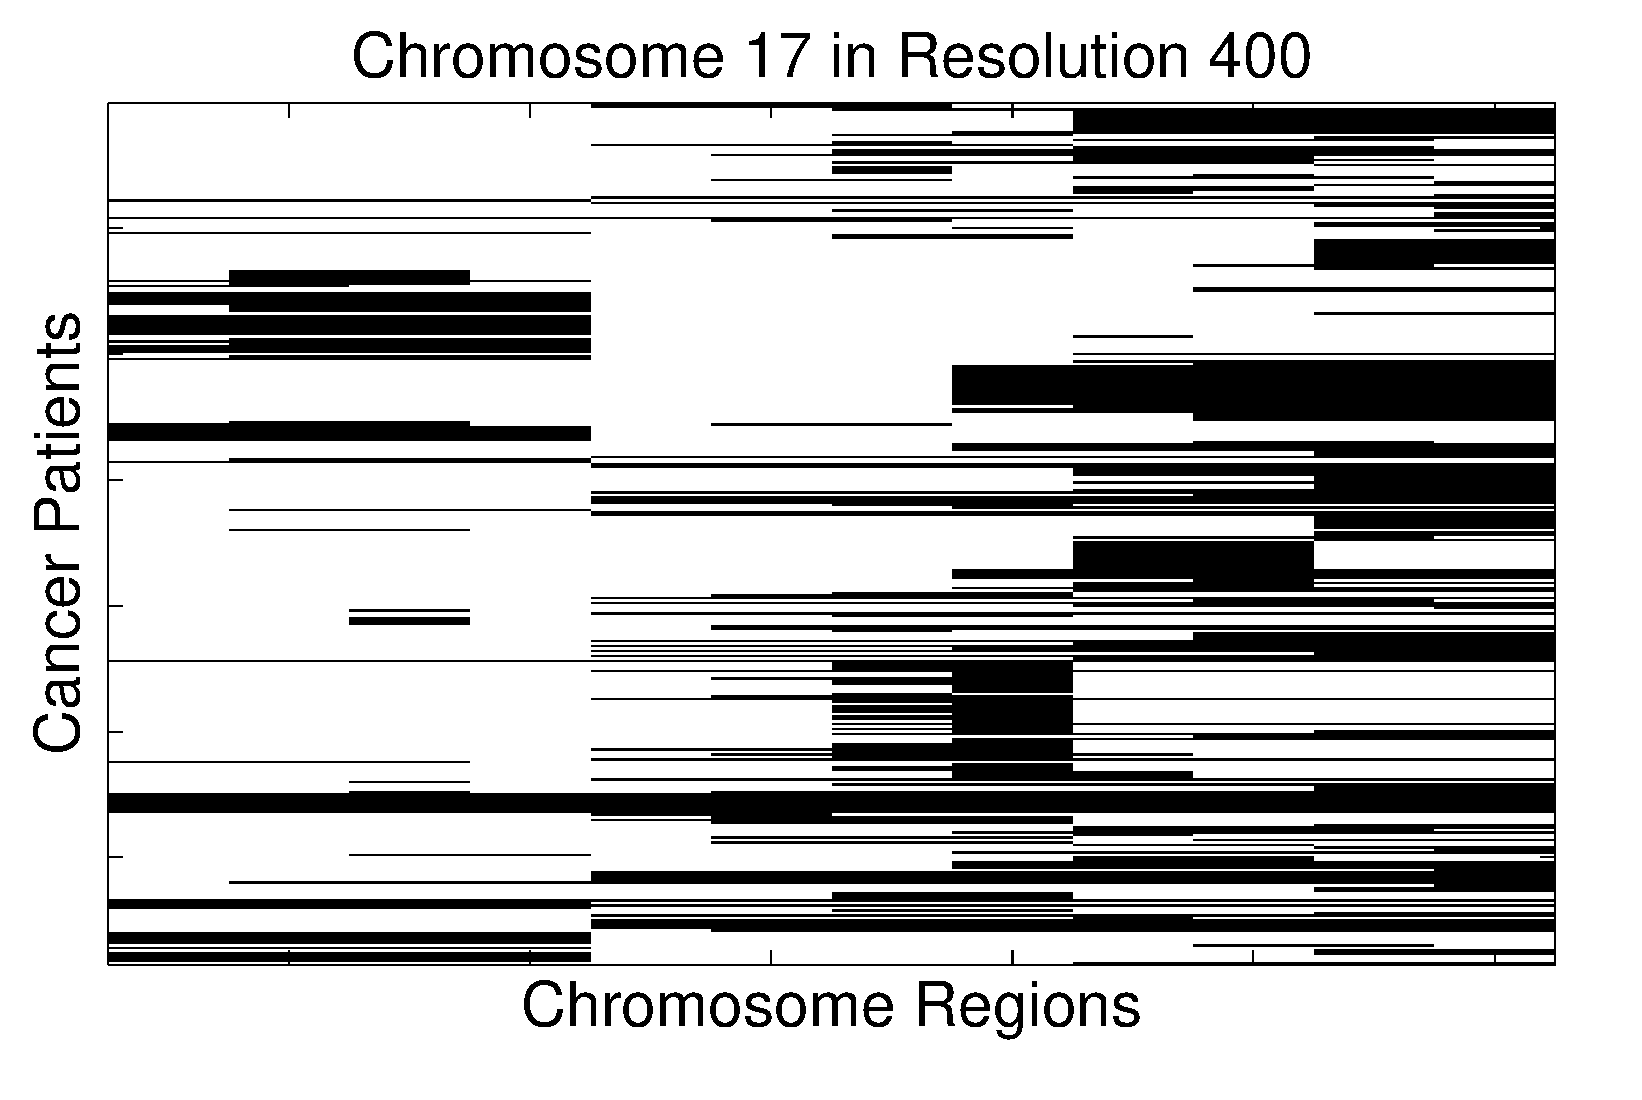
\includegraphics[width=0.9\textwidth]{figures/chr17dm400}
\caption[Aberrations in chromosome 17 in resolution 400]{DNA copy number aberrations in chromosome 17, resolution 400. $\overline{X}=(X_{ij})$, $X_{ij}\in \{0,1\}$. Each row represents one sample of the aberrations pattern for a cancer patient and each column represents one of the chromosome bands (regions). In figure dark color denotes the presence of aberrations and the white color denotes the absence of chromosomal aberrations.} \label{Fig:data}
\end{figure}

The dataset used in the experiments defines DNA copy number aberrations in different chromosomes. The data was collected by the bibliomics survey of 838 journal articles during 1992-2002 by hand without using state-of-the-art text mining techniques~\cite{Myllykangas200815, Holl20071}. The dataset contained the information about the chromosomal aberrations of 4590 cancer patients. Each row describes one sample of the cancer patient while each column identifies one chromosomal band(region). The dataset is a typical \mbox{0-1} dataset where aberrated chromosomal regions were marked with 1 while and the value 0 defines that the chromosome band is not aberrated.  Chromosomes X and Y were not included in the experiments because of the lack of data. Patients whose chromosomal band had not shown any aberrations for the specific chromosome were not included in the experiments since we are interested in modelling the aberrations, not their absence. Thus different chromosomes had different number of the samples. The chromosomal aberrations dataset analyzed in this thesis uses data containing few samples. Thus, we decided to work chromosomewise because of the availability of very small number of the data samples to constrain the complexity of the mixture models. The original data dimension for the whole genome ranges from 300 to 850 which will be cumbersome to work with given the very large dimension compared to the number of samples. On the other hand, working with each chromosome will be computationally easier as the largest dimensionality is 63.


\begin{figure}[h!]
\centering
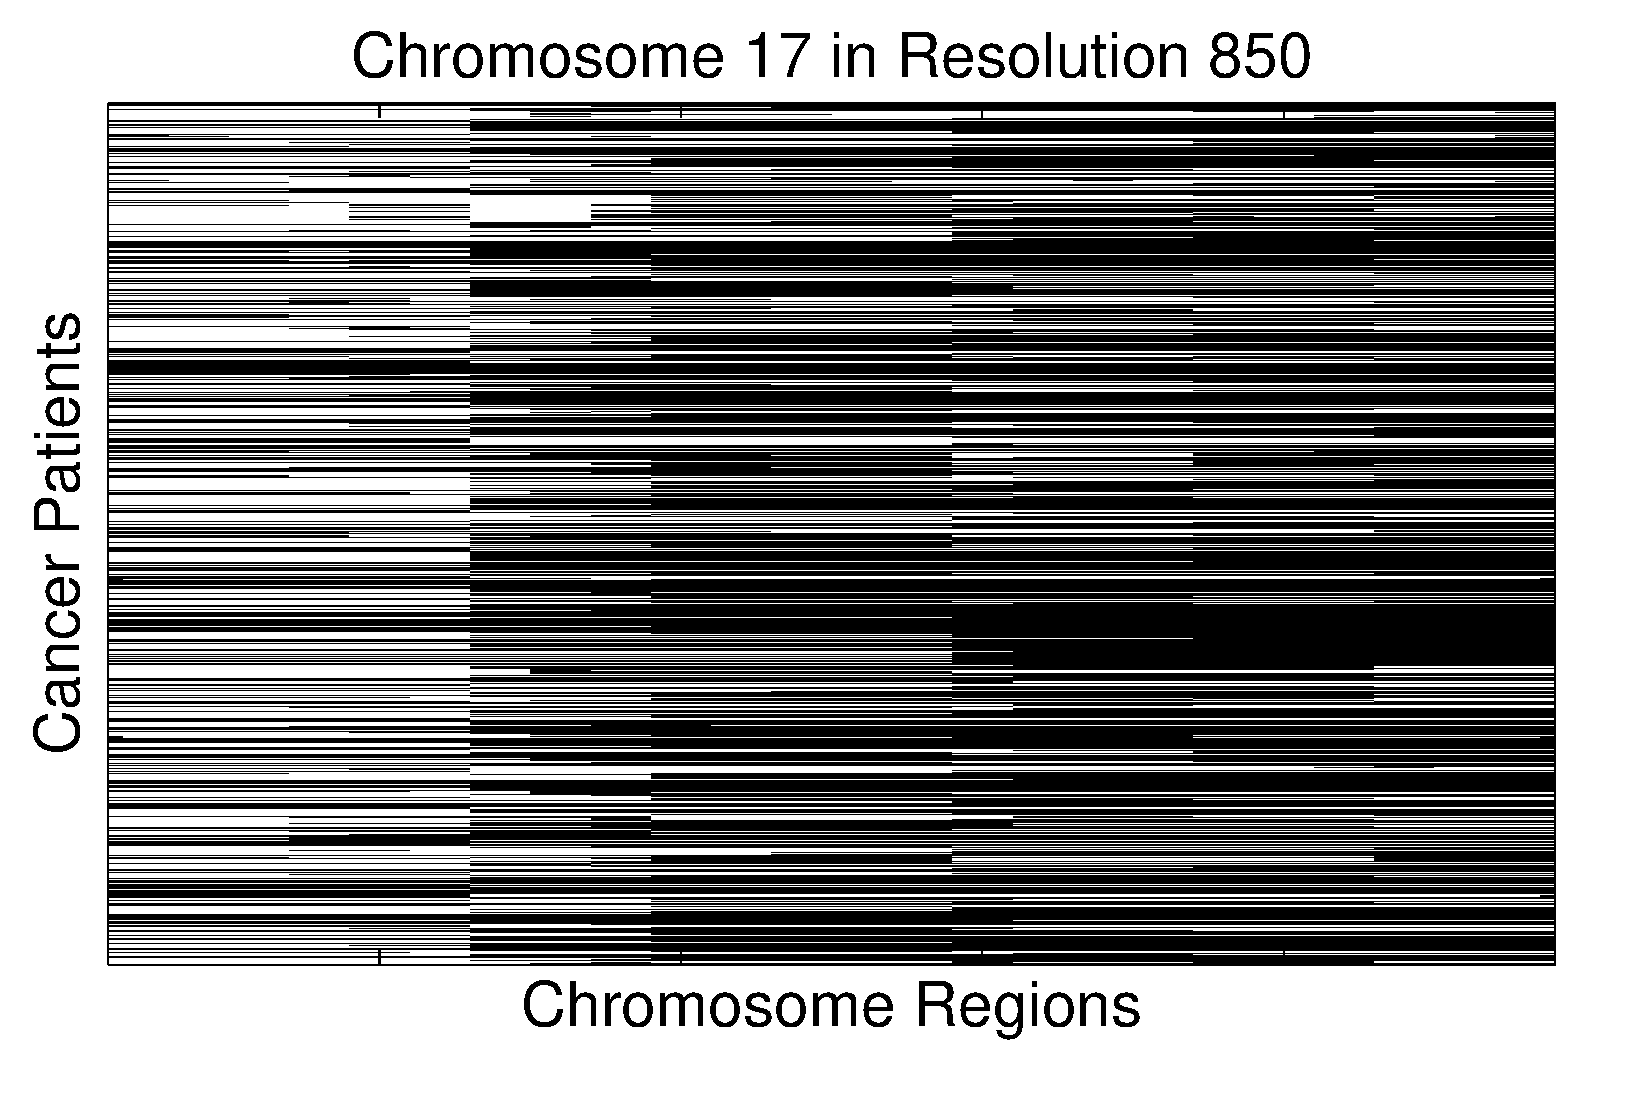
\includegraphics[width=0.9\textwidth]{figures/chr17dm850data}
\caption[Aberrations in chromosome 17 in resolution 850]{DNA copy number aberrations in chromosome 17, resolution 850. $\overline{X}=(X_{ij})$, $X_{ij}\in \{0,1\}$. Each row represents one sample of the chromosomal aberrations for a cancer patient and each column represents one of the chromosome bands (regions).  In figure dark color denotes the presence of aberrations and the white color denotes the absence of chromosomal aberrations.} \label{Fig:data850}
\end{figure}

A shwon in Figures~\ref{Fig:data} and~\ref{Fig:data850}, copy number aberrations occur very sparsely and are often spatially dependent. The original data was in the resolution 400 i.e. there were 393 chromosomal bands (regions) for the entire genome. The original data was upsampled to resolution 550, 700 and 850 and downsampled to resolution 300 using the methods discussed in Chapter~\ref{ch:sampling}. Bands for the specific chromosome were extracted and mixture modelling was preformed on each chromosome. For example: chromosome 1 had 63, 61, 42, 28, and 23 chromosomal bands in resolution 850, 700, 550, 400, and 300 respectively~\cite{iscn}. Similarly, a different set of data was available in resolution 850 from progenetix.net~\cite{progenetix}. The data in resolution 850 was different from data in resolution 400. Similar to the data in the resolution 400, the data in resolution 850 was downsampled to resolution 300, 400, 550 and 700. Elementwise AND operation over all the samples in the data results in a zero vector thus  necessitating sophisticated machine learning and data mining methods and techniques for classifying and profiling aberrations.

The ISCN (ISCN 2009: An International System for Human Cytogenetic Nomenclature) nomenclature of chromosome, discussed in Appendix~\ref{ap:appendNom}, divides the chromosome into different resolutions shown in Table~\ref{Tab:resolution}.
\begin{table}[h!]
  \centering
\begin{tabular}{ |c|c|c|c| }
\hline
  \textbf{S.No} &  \textbf{Resolution} &\textbf{$\#$ Regions} &\textbf{$\#$ Regions in Chr 1 } \\ \hline \hline
  1& 300 & 317 & 23\\ \hline
  2& 400 & 393 & 28\\ \hline
  3& 550 & 555 & 42\\ \hline
  4& 700 & 759 & 61 \\ \hline
  5& 850 & 862 & 63 \\ \hline
\end{tabular}
\caption[Chromosomal regions in different resolutions]{Number of Chromosome bands(regions) for 5 different resolutions of data studied in the thesis. Included as an example number of bands in Chromosome 1, the largest chromosome.}
\label{Tab:resolution}
\end{table}

Thorough study was performed for every chromosome with every resolution using the finite mixture modelling approach.

\section{Comparison of Downsampling Methods}
\label{s:comparisionMethods}
The downsampling methods, discussed in Chapter~\ref{ch:sampling}, were implemented in scripts. There were 110 scripts in all for all transformations, one for each chromosome in 5 different resolutions (\# of Chromosomes $\times$ \# of Resolutions i.e $22 \times 5$). Matlab \textregistered~\cite{matlab} was used for scripting. The individual scripts for downsampling each chromosome takes a file name of the data set in higher resolution as input and first checks for some errors such as mismatch in the number of regions of the chromosome in that specific resolution. Data is then transformed bandwise to lower resolution combining the multiple bands in higher resolution according to the three different methods proposed in Sections~\ref{ss:orfunction},~\ref{ss:majority}, and~\ref{ss:weighted}. The downsampled data from 850 resolution was subjected to various tests to access the difference in the results of the downsampling methods. 

\subsection{Property Models}
\label{ss:totamplification}
Some simple and efficient property models were defined to compare the results of the three different downsampling procedures. 

\subsubsection{Column and Row Margins}
\label{sss:rowcolmargins}

\begin{figure}[h!]
\centering
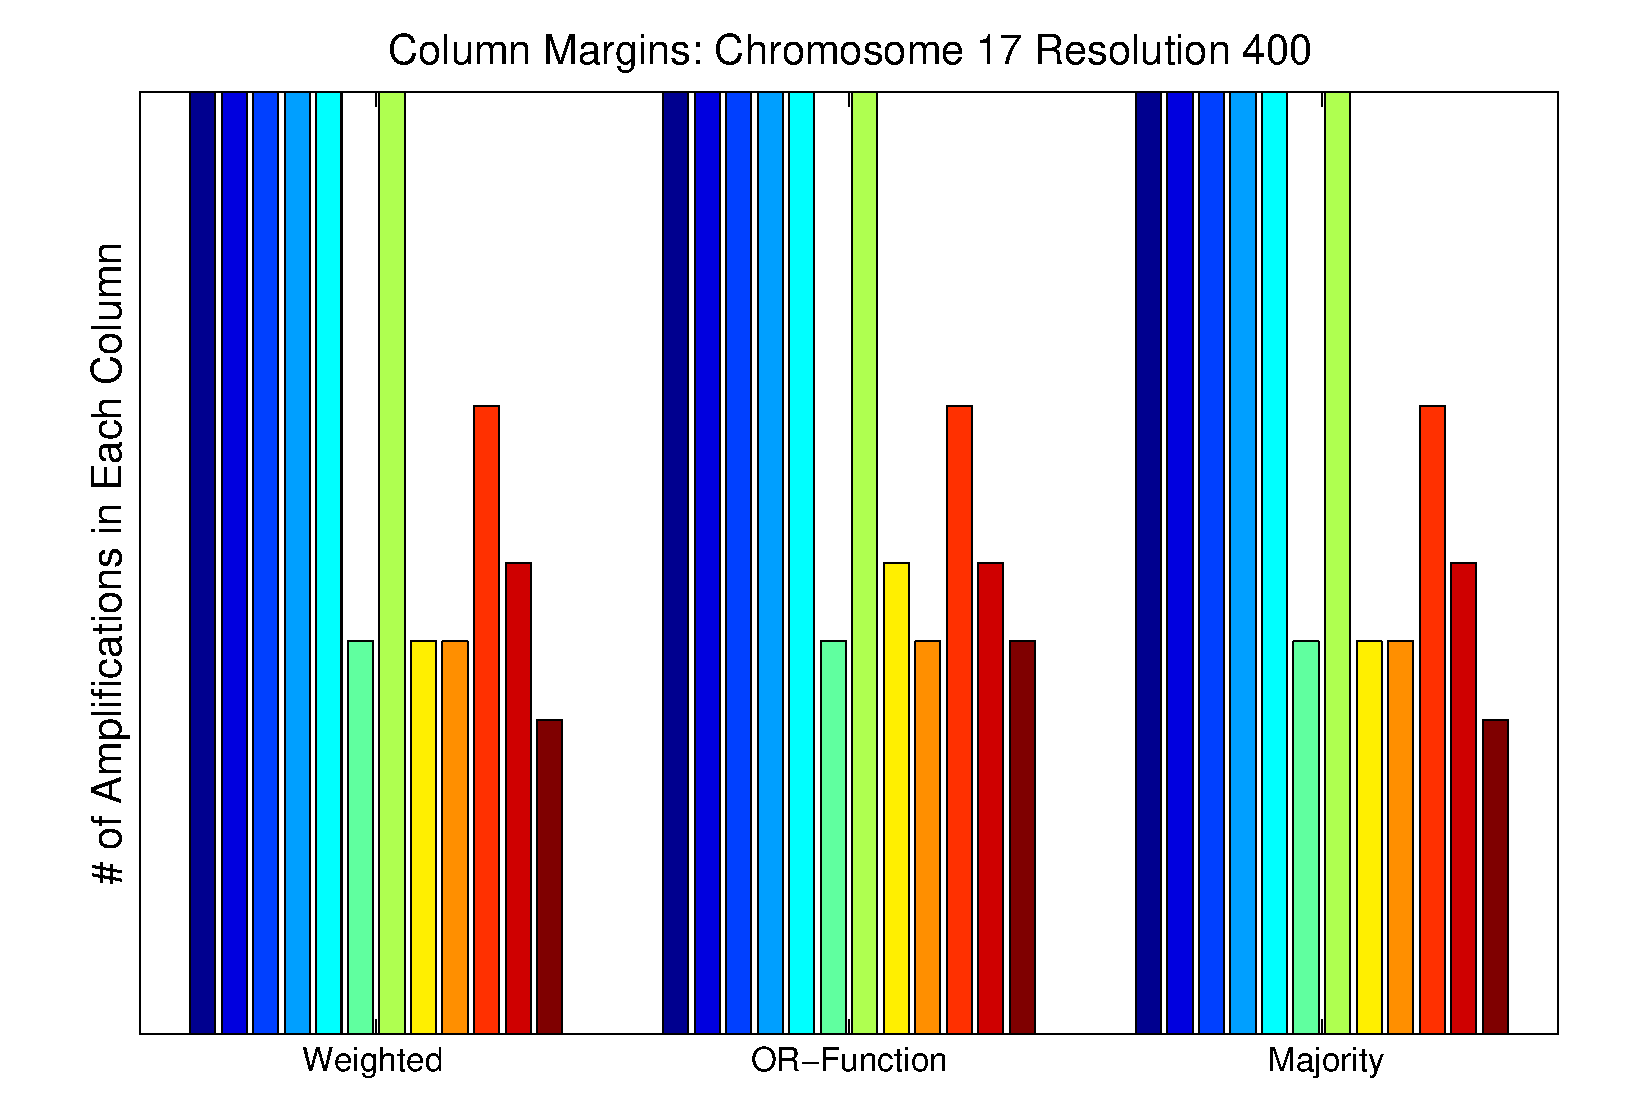
\includegraphics[width=0.9\textwidth]{figures/columnsumChr17}
\caption[Aberrations in each column]{Comparison of three different downsampling methods: Example case in chromosome 17 resolution 400. Figure does not show significant difference in the results of the three methods.}\label{Fig:histchr6dm393}
\end{figure}

The total number of differences in the dataset was studied with respect to each row and column margin produced on downsampling from higher resolution to lower resolution. The total number of differences in each chromosome band and in each cancer patient was computed and compared between three different downsampling methods. The results of the three different downsampling process did not show significant differences with respect to the number of differences in the row and column margins as shown in Figure~\ref{Fig:histchr6dm393} which is an example result for chromosome 17 in resolution 400. Figure~\ref{Fig:histchr6dm393} shows that results produced by three methods are highly similar. In order to scrutinize the results, mean difference between the number of differences produced by the three methods in various chromosome bands was computed. The results for an example case discussed earlier i.e. chromosome 17 in resolution 400 is shown in the Figure~\ref{Fig:diffchr6dm393}. 


\begin{figure}[h!]
\centering
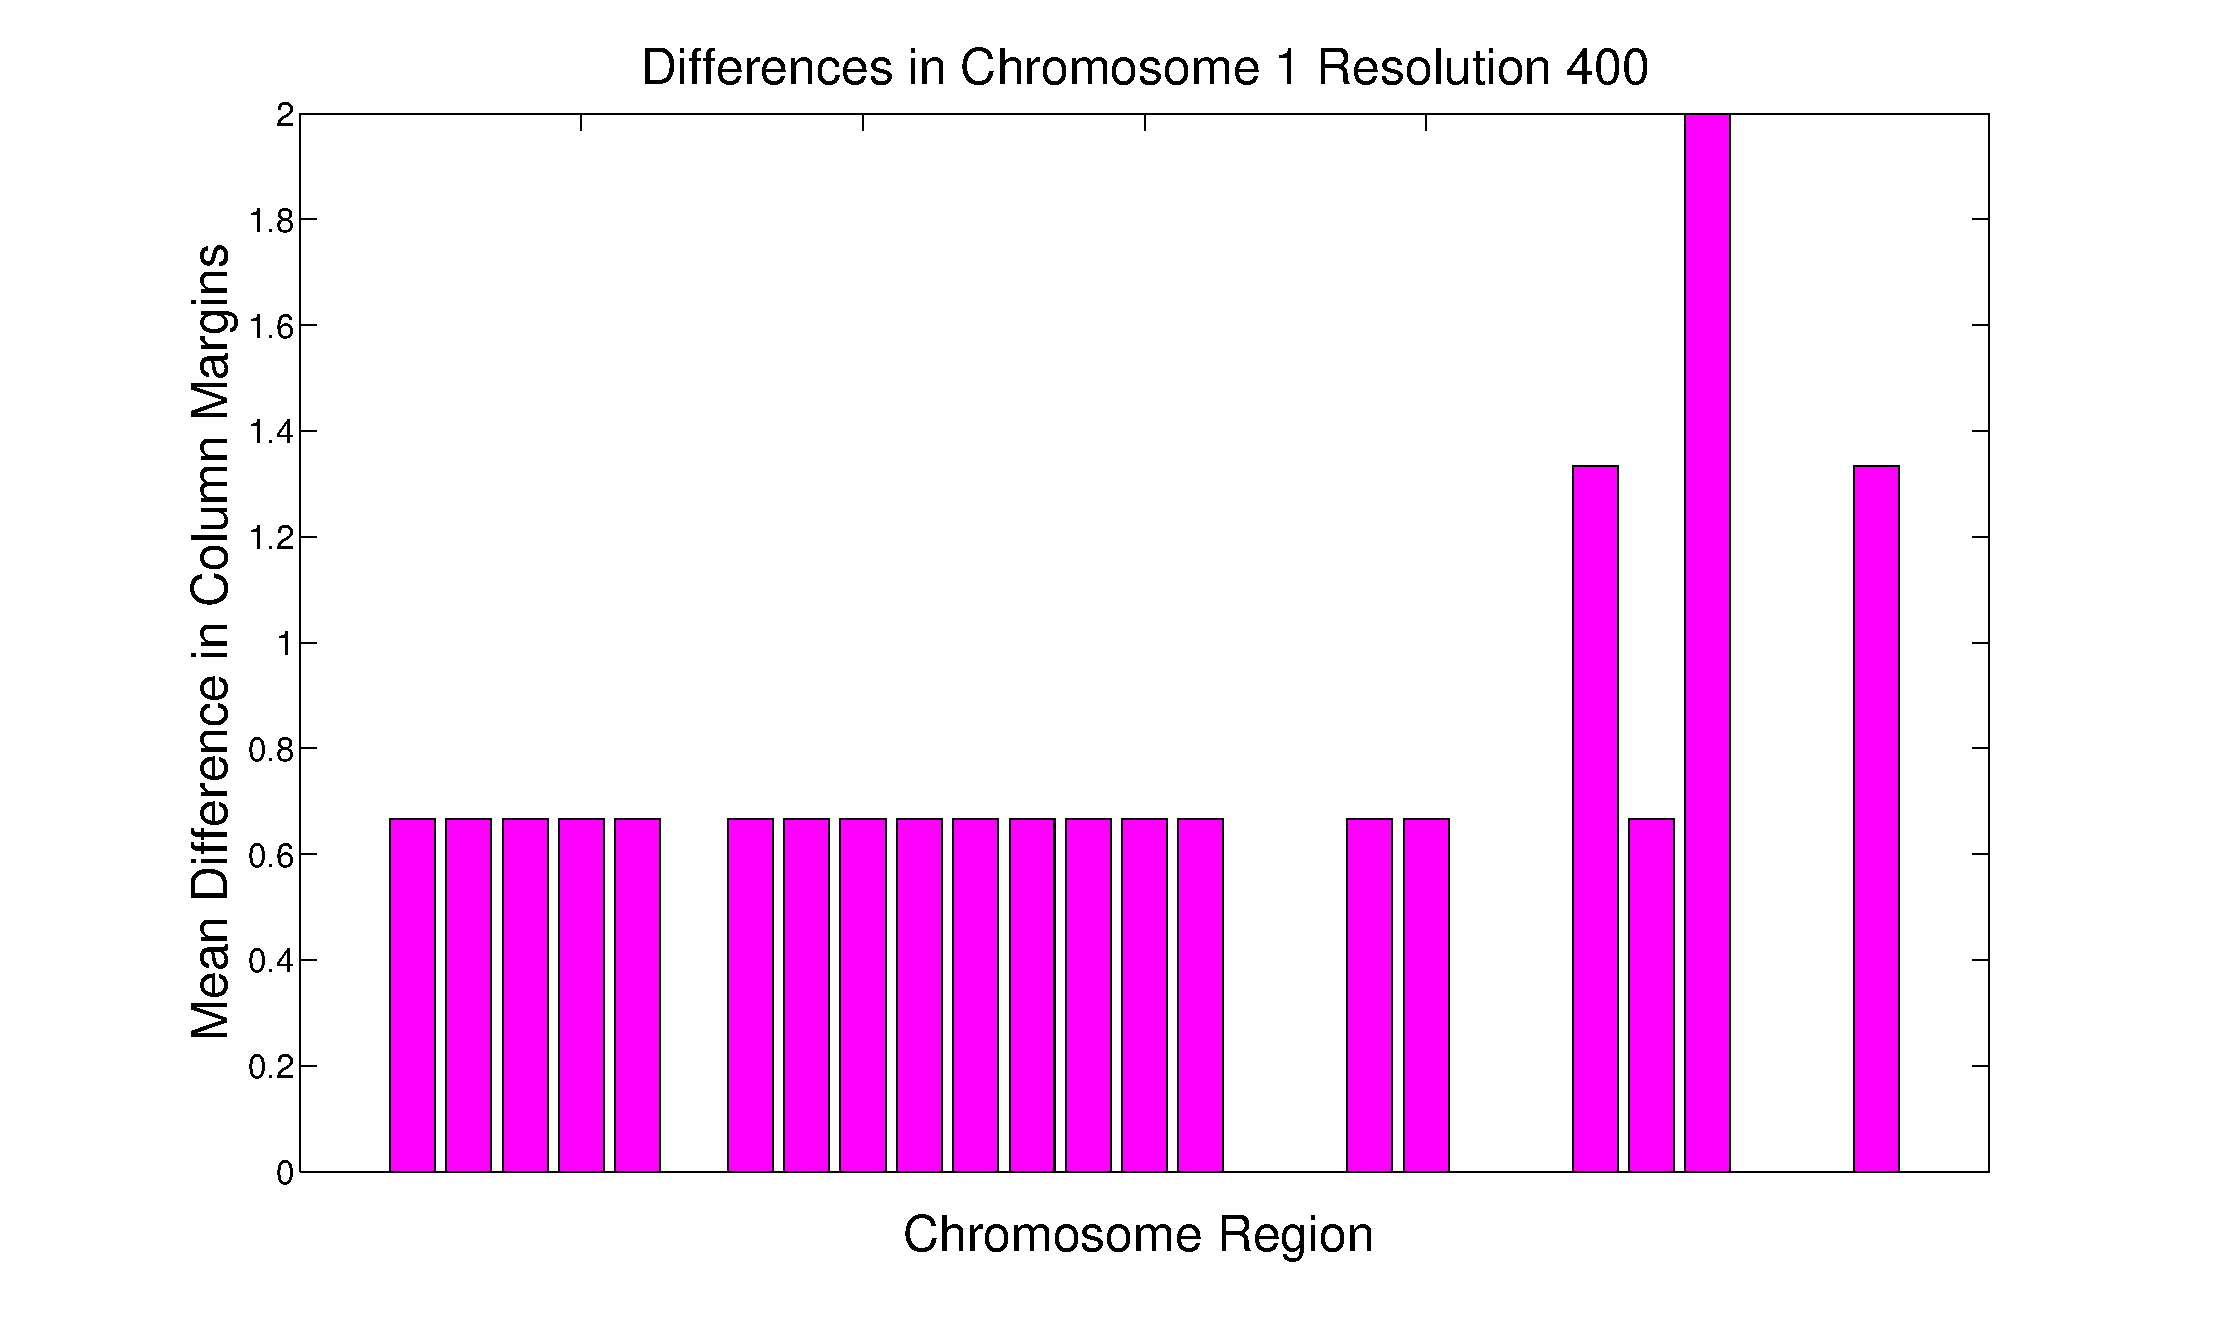
\includegraphics[width=0.9\textwidth]{figures/meanColumnMardiffChr1}
\caption[Mean of differences in aberrations in each column]{Total difference in data produced by three different downsampling methods: Example case in chromosome 1 resolution 400. The figure shows presence of  differences in some chromosome regions.}\label{Fig:diffchr6dm393}
\end{figure}


Figure~\ref{Fig:diffchr6dm393} suggests that there are differences in the results produced by three downsampling methods albeit rather minute. Three downsampling methods produced no differences in some chromosomes such as chromosome 1, 5, 8, 19, 20, 21 and 22 in resolution 700. In contrast, the methods produced some negligible differences in other chromosomes. Hence with respect to the total number of differences in row and column margins produced in the coarse resolution, the three proposed methods are highly similar.

\subsubsection{Total Number of Differences}
\label{ss:totaldifferences}

\begin{figure}[h!]
\centering
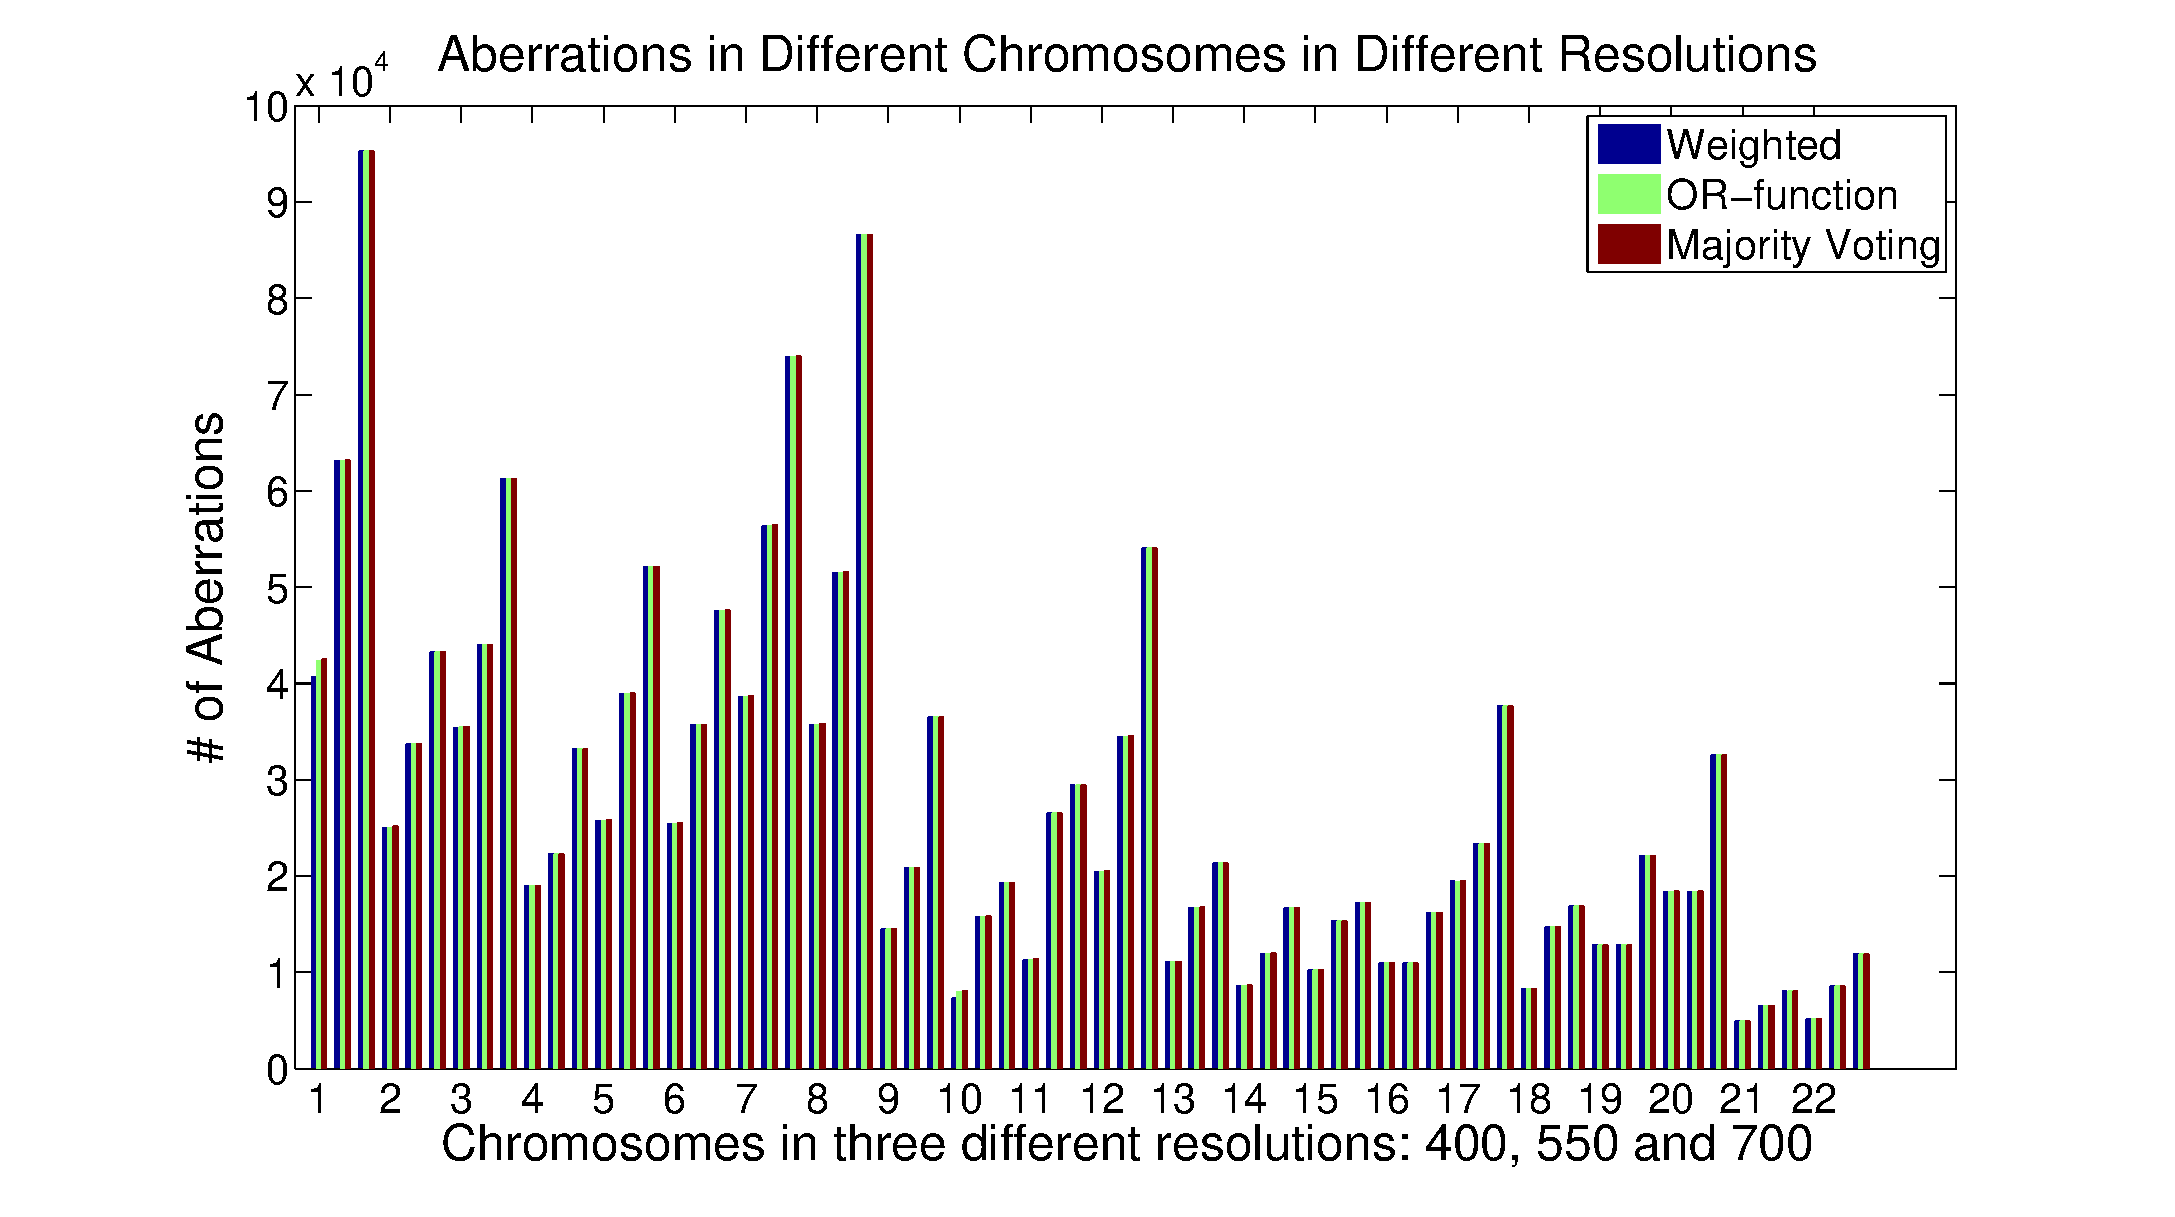
\includegraphics[width=0.9\textwidth]{figures/abrdiffres1}
\caption[Number of aberrations produced]{Comparison of three different downsampling methods with respect to number of aberrations produced.}\label{Fig:total1hist}
\end{figure}

Similar to the differences in datasets, we studied the total number of aberrations present in the downsampled data. Total number of aberrations in each chromosome was computed and compared between three different downsampling methods. The results of the three different downsampling methods did not show significant differences with respect to the number of aberrations produced. Figure~\ref{Fig:total1hist} suggests that the three downsampling methods produces similar results. Furthermore, the mean difference between the number of aberrations produced by the three methods in various chromosomes was computed.

\begin{figure}[h!]
\centering
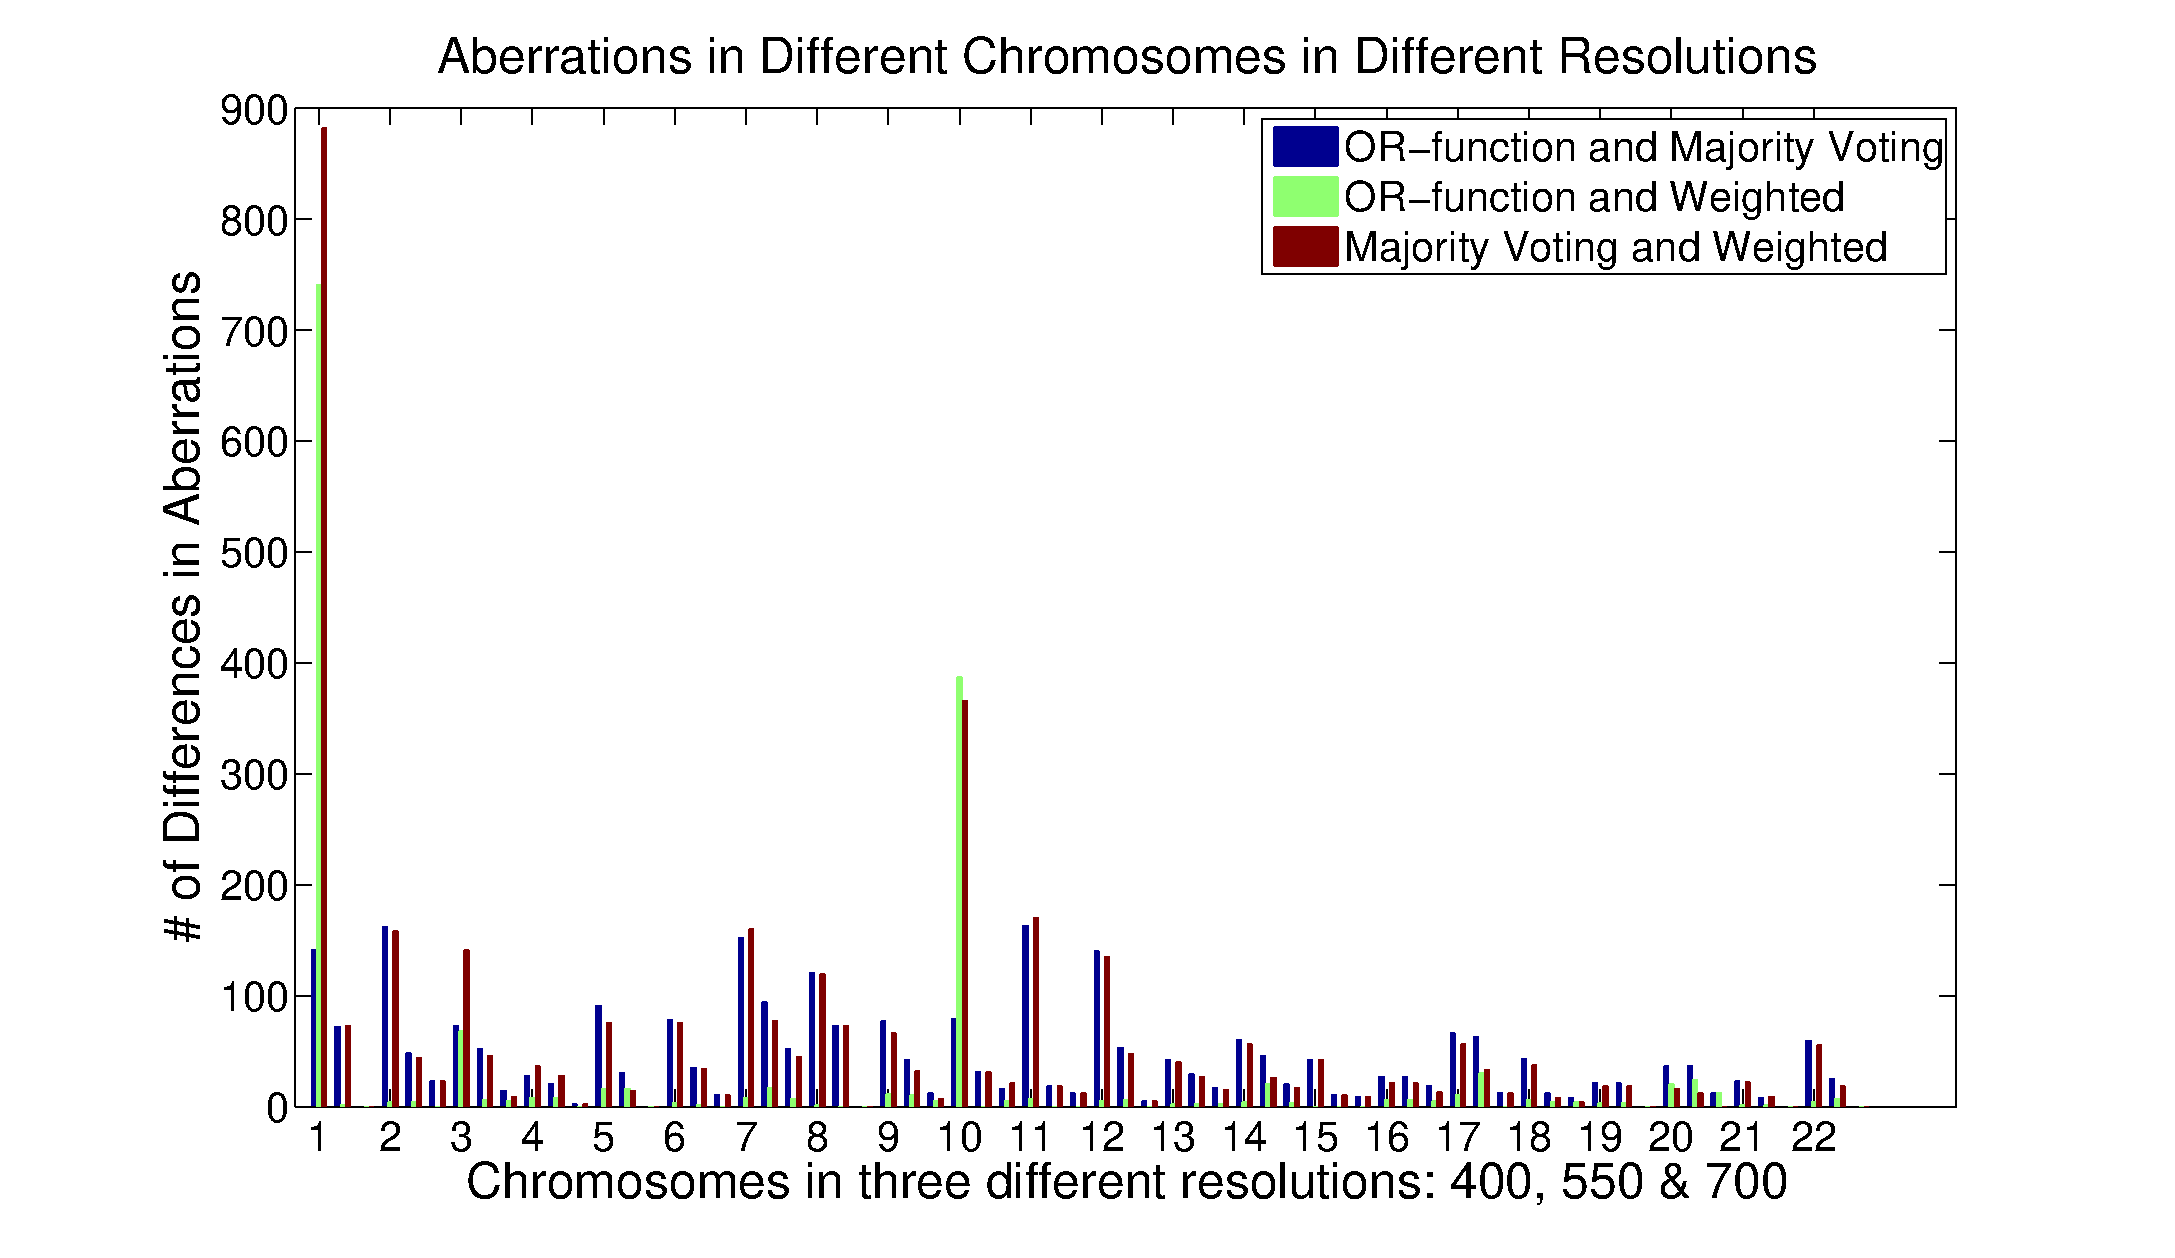
\includegraphics[width=0.9\textwidth]{figures/diffaberrations1}
\caption[Mean differences in the aberrations produced]{Difference in aberrations produced by three different downsampling methods with respect to the number of aberrations produced in the data.} \label{Fig:total1diff}
\end{figure}

Figure~\ref{Fig:total1diff} suggests that there are differences in the results produced by three downsampling methods, albeit very small. However, the differences between the methods are not significant when the number of aberrations are considered, which are significantly high.

%\clearpage

% \subsection{Number of unique rows}
% \label{ss:uniquerows}
% 
% As discussed in Section~\ref{s:dataset}, the chromosomal aberrations dataset was a \mbox{0-1} dataset consisting of chromosomal aberrations in cancer patients. Since the chromosomal aberrations are rare and data was high dimensional, the number of unique rows have high significance especially in clustering. 
% Hence, the number of unique rows in the downsampled data was compared. Similar to the total number of chromosomal aberrations, the number of unique rows in the downsampled data did not exhibit significant differences as depicted in the Figure~\ref{Fig:unqrowhist}.
% 
% \begin{figure}[h!]
% \centering
% 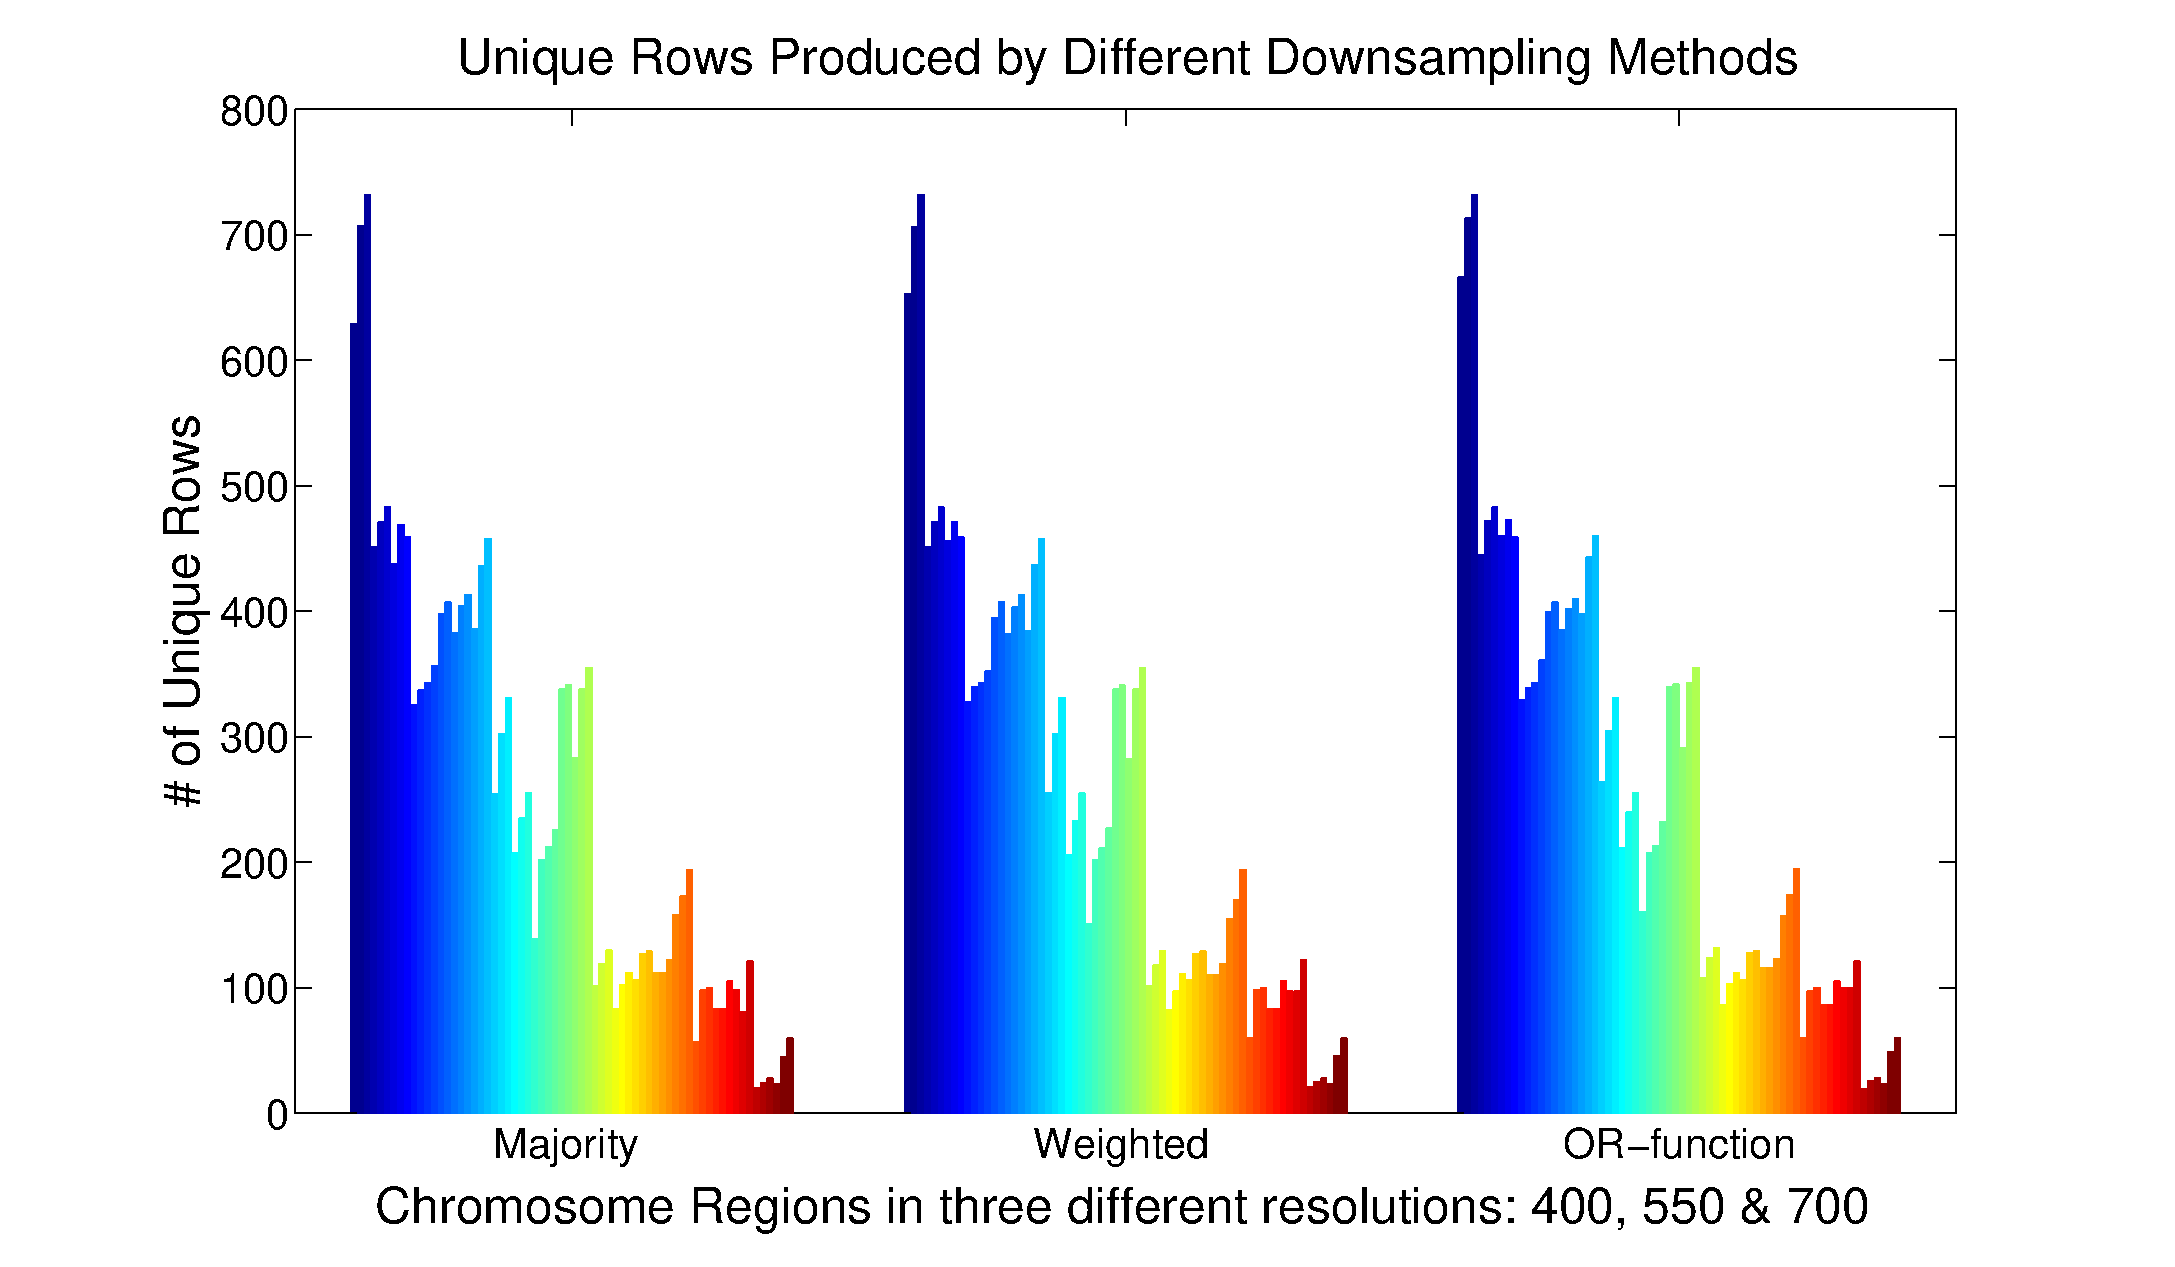
\includegraphics[width=0.9\textwidth]{figures/unqrows1}
% \caption[Unique rows produced]{Number of unique rows produced by three different downsampling methods. X-axis varies in small intervals with respect to resolution and larger intervals with respect to the chromosome number.}\label{Fig:unqrowhist}
% \end{figure}
% 
% Figure~\ref{Fig:unqrowhist} indicates that the number of unique rows produced by three different downsampling methods does not vary in different methods. Similar, to the total number of aberrations discussed in Section~\ref{ss:totamplification}, the results were further scrutinized calculating the mean of differences of the number of unique rows produced by each method in each chromosome for each resolution. Figure~\ref{Fig:uniqrowdiff} portrays the mean of differences in number of  unique rows produced by each downsampling method.
% 
% \begin{figure}[h!]
% \centering
% 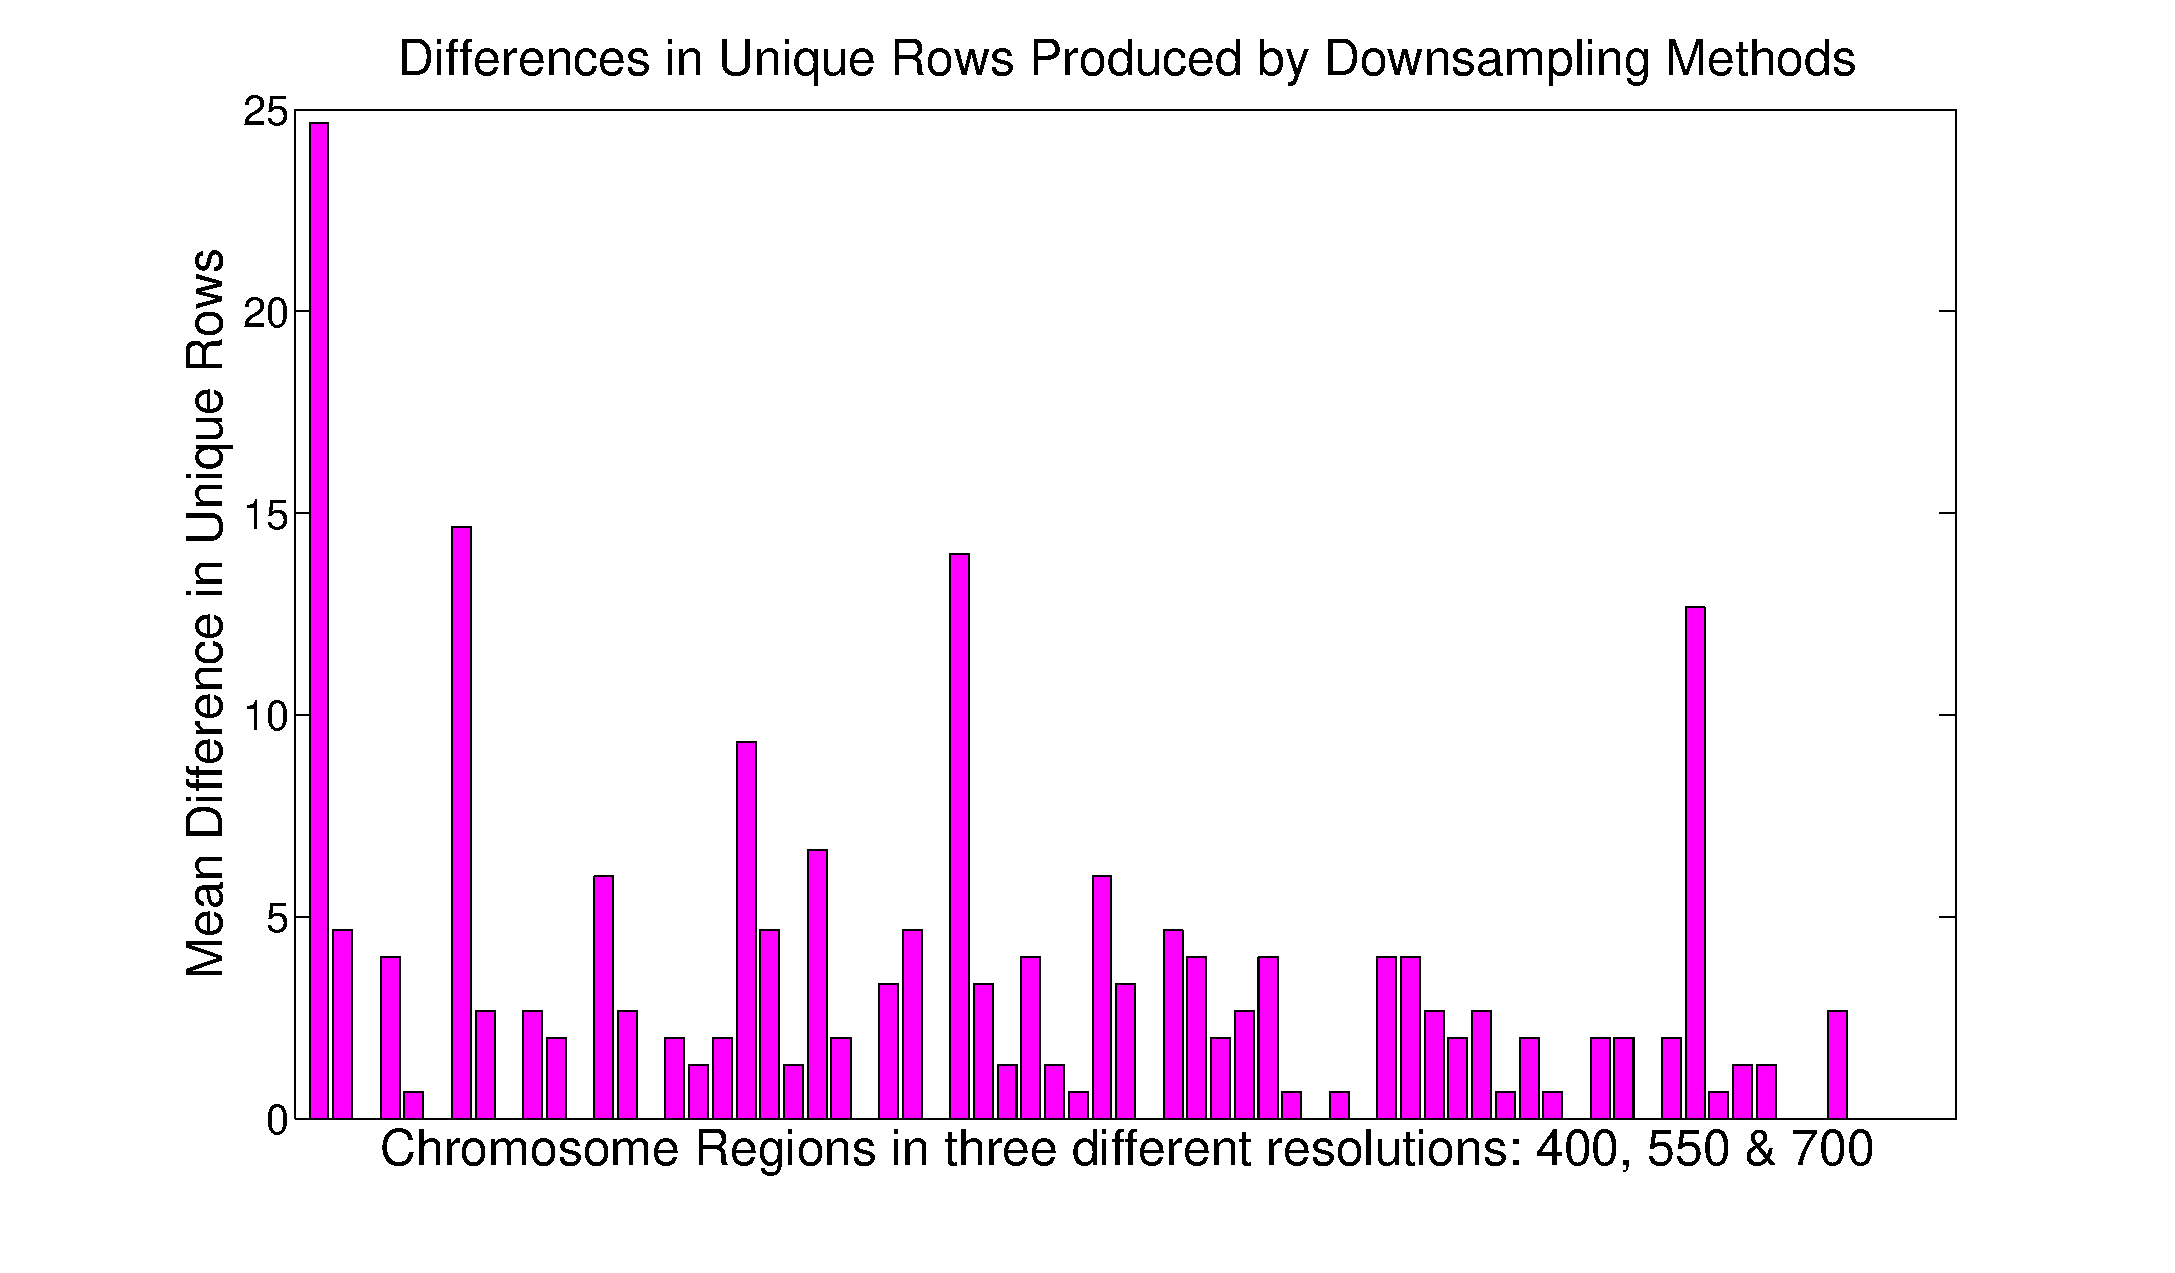
\includegraphics[width=0.9\textwidth]{figures/diffunqrows1}
% \caption[Differences in unique rows produced]{Mean of difference in number of unique rows produced by three different downsampling methods. The X-axis varies in small intervals with respect to resolution and larger intervals with respect to the chromosome number.} \label{Fig:uniqrowdiff}
% \end{figure}
% 
% Figure~\ref{Fig:uniqrowdiff} shows that the number of unique rows varies in some chromosomes. However, these differences are negligible and the overall picture demonstrates no significant differences in the result of three different downsampling methods with respect to the number of unique rows produced in downsampled data.


\subsection{Matrix Difference: Frobenius Norm}
\label{ss:0to1}
Property models discussed in Section~\ref{ss:totamplification} demonstrate no significant differences in the downsampling methods. However, the two methods discussed in Section~\ref{ss:totamplification} are susceptible to some errors where the number of chromosomal aberrations are same and also number of chromosomal aberrations does not change in different methods. For example, the methods discussed Section~\ref{ss:totamplification} do not show difference between the following two datasets. 

\begin{equation*}
  \begin{bmatrix}
    1 & 0  \\
    0 & 1  \\    
  \end{bmatrix} \mbox{ and }
   \begin{bmatrix}
   0 & 1  \\
   1 & 0  \\    
  \end{bmatrix}
\end{equation*}

However, the two datasets above are significantly different. In order to capture these differences, we further analyzed the difference between the different downsampling methods as the difference between the two resulting matrices for different methods using standard matrix difference measures. The distance measure used is the square of the Frobenius norm~\cite{frobenius} between two matrices. In \mbox{0-1} matrices, Frobenius norm is essentially the number of cells where the two matrices differ. 

\begin{figure}[h!]
\centering
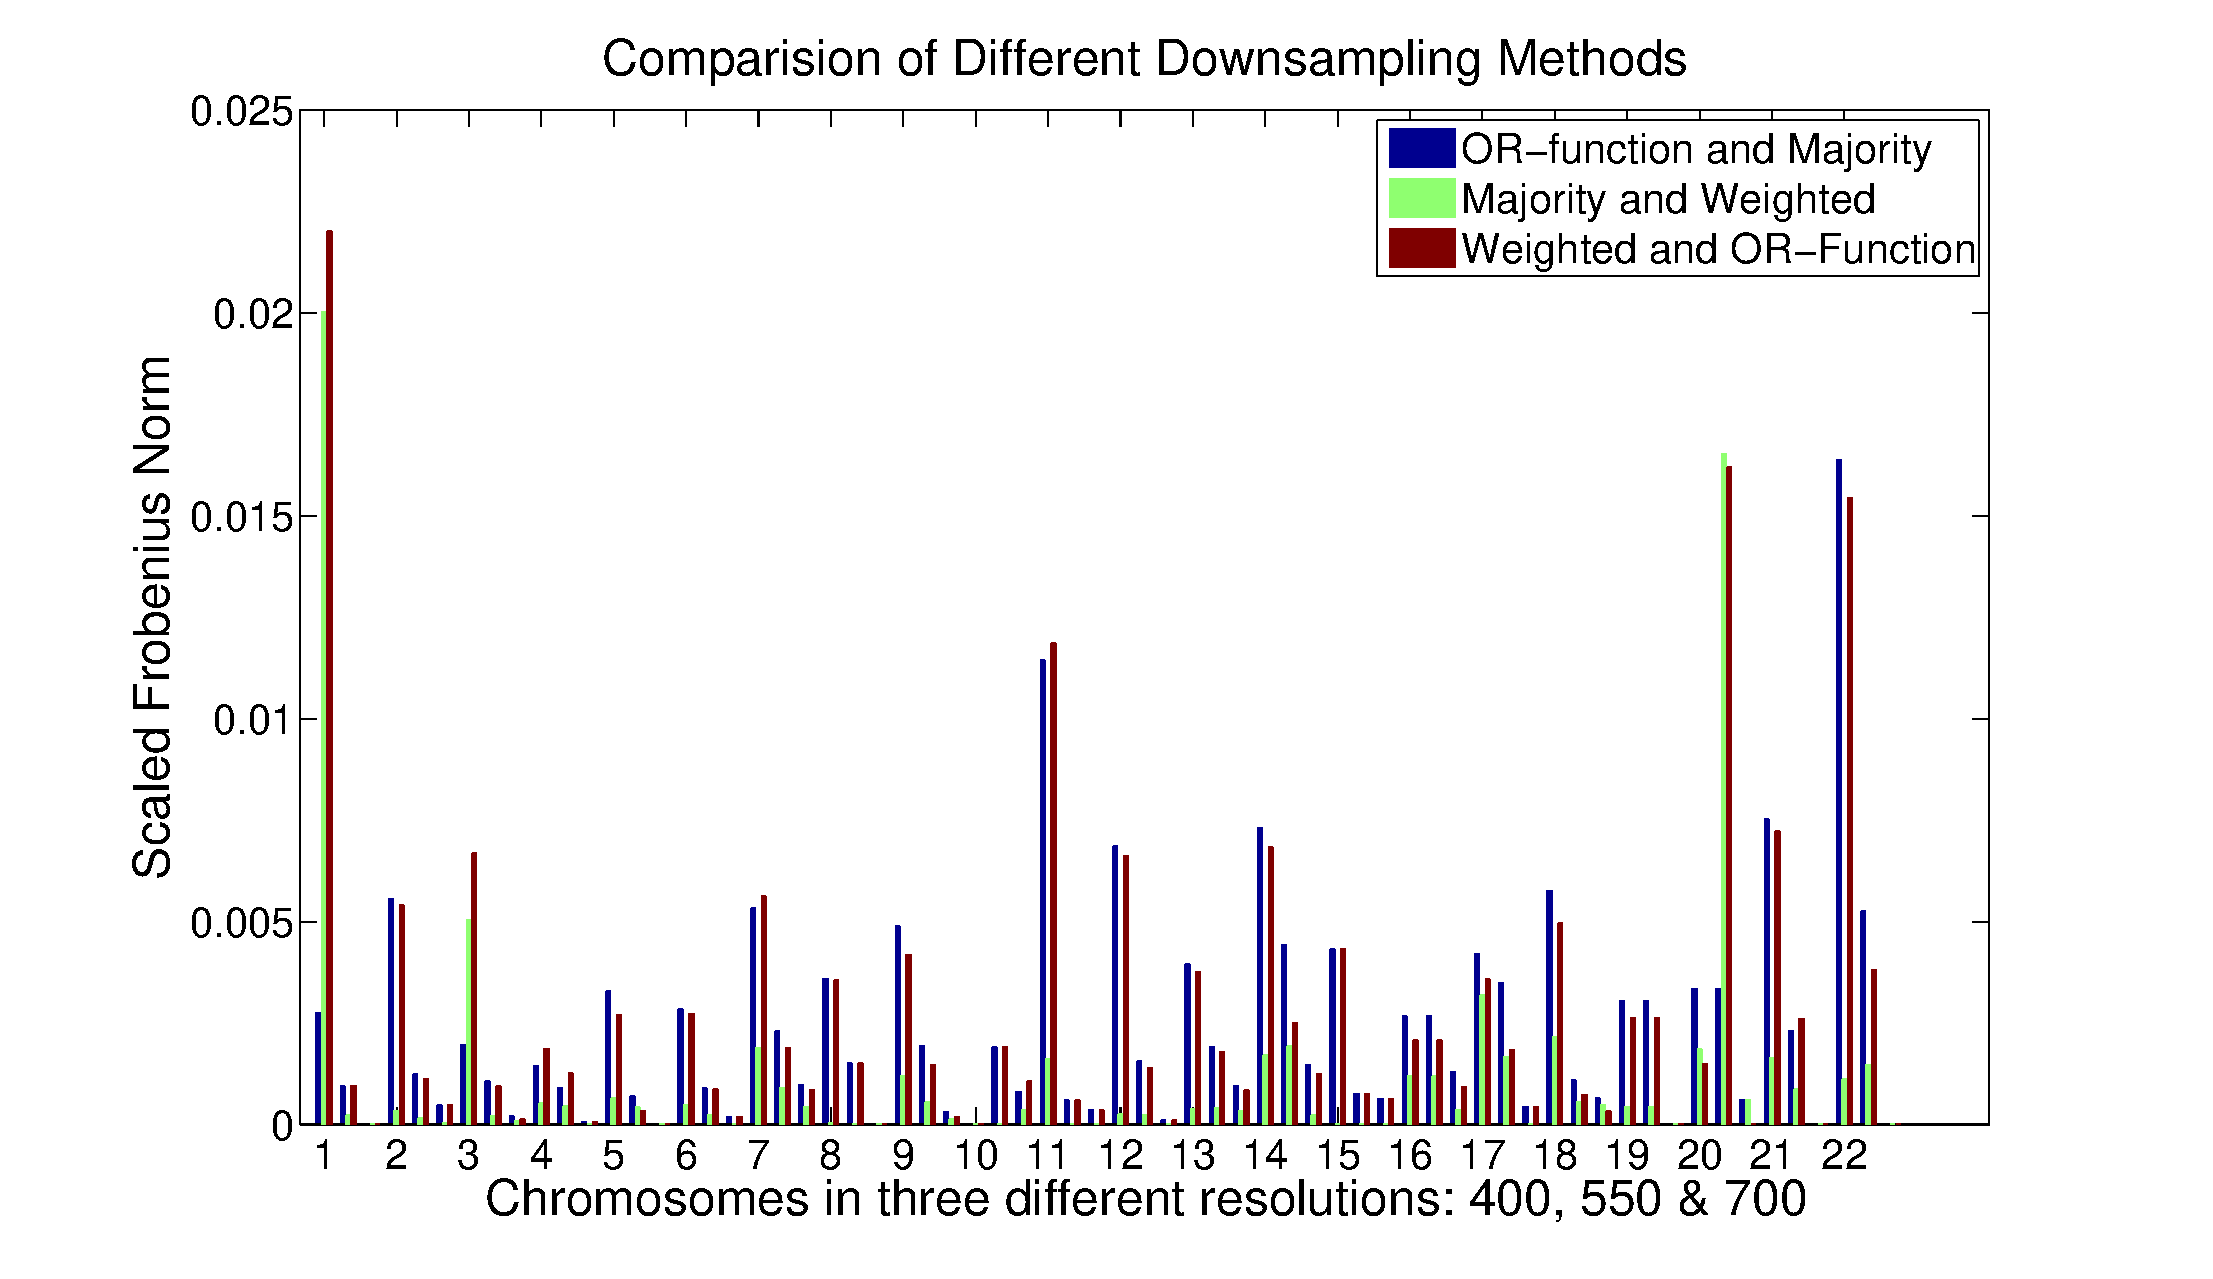
\includegraphics[width=0.9\textwidth]{figures/frobeniusnorm1}
%\epsfig{file=figures/frobenius.eps, height=2.2in, width=3.2in}
\caption[Frobenius norm]{Comparison of three different downsampling methods: The difference measure used is scaled Frobenius norm.}\label{Fig:frobenius}
\end{figure}

Figure~\ref{Fig:frobenius} suggests that the three downsampling methods produces fairly similar results. It also suggests that the differences are high in chromosome 1 which is expected because chromosome 1 is the largest chromosome. Differences are also high in lower resolution compared with higher resolution because it is the lower resolution where most of the changes take place. The differences in the smaller chromosomes especially 20-22 are because of significant variation in the bands combined. Normally, three bands in finer resolution are combined in coarser resolution but in small chromosomes, the number of chromosome bands combined is very different thus making it difficult for weighted and OR-function downsampling method to work. It is to be noted that in the chromosomes where the differences are larger have larger number of differences in number of chromosome bands in different resolutions. 

\subsection{Changes in Aberrations}
\label{ss:chinaberrations}
We also calculated the number of cases where the unaberrated band has changed to the aberrated region in two different methods. Calculating such differences will also help to measure the closeness of different downsampling methods. The number of cases where the unaberrated region (represented by 0 in dataset) changes to the aberrated band (represented by 1 in dataset) is calculated and the results are visualized as shown in the Figure~\ref{Fig:0to1hist}.
\begin{figure}[h!]
\centering
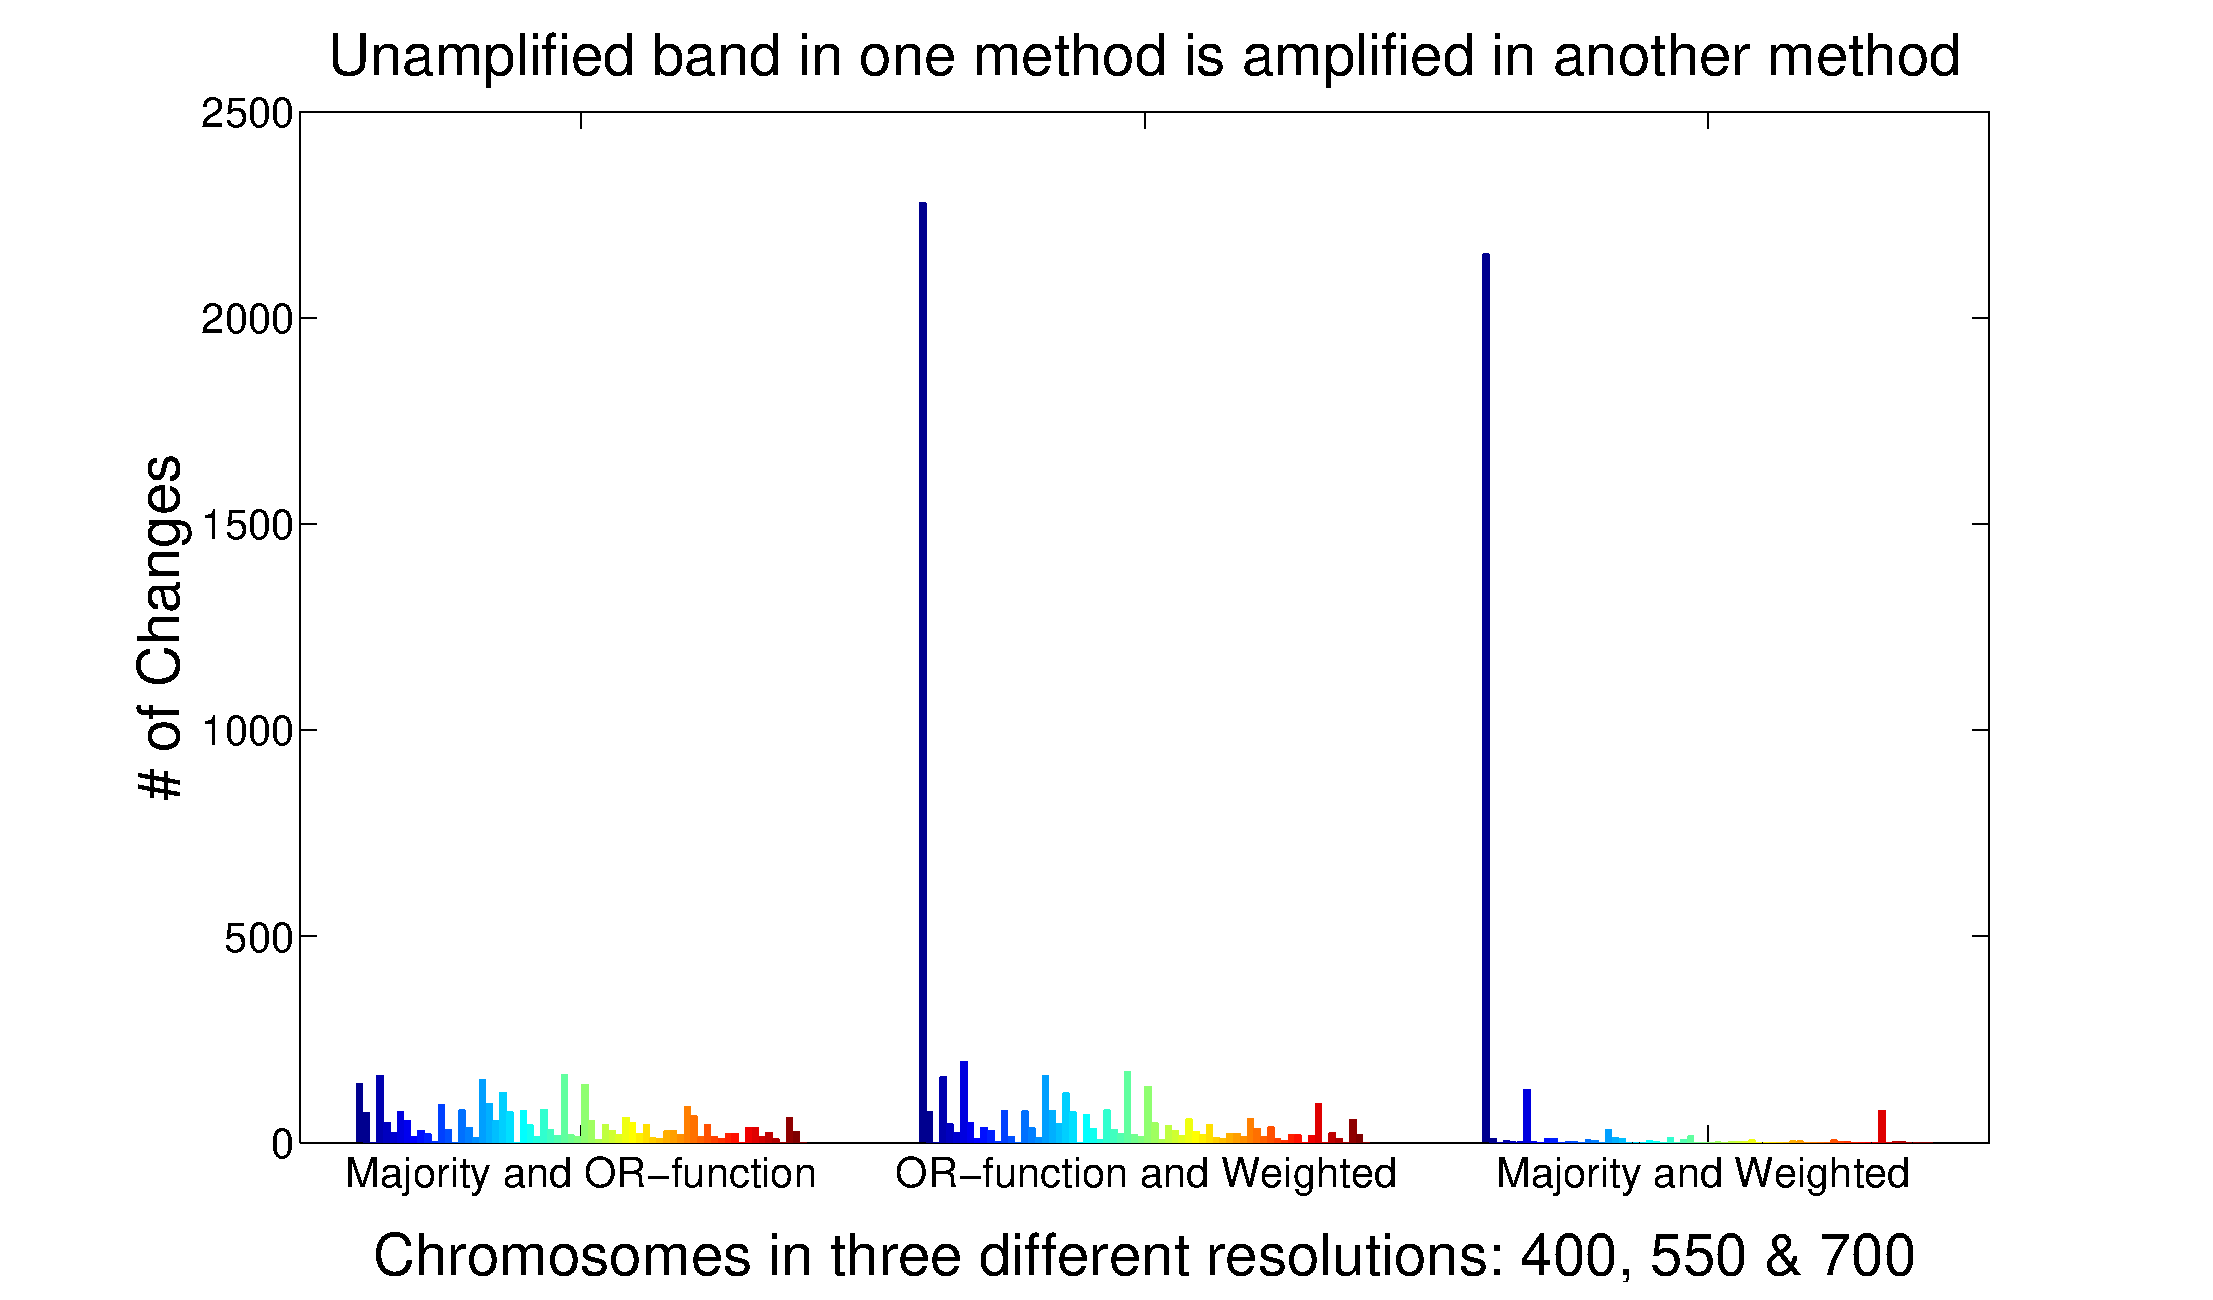
\includegraphics[width=0.9\textwidth]{figures/0to1changes1}
\caption[Number of \mbox{0-1} changes]{Number of unaberrated bands changing to aberrated bands in different downsampling methods. The X-axis varies in small intervals with respect to resolution and larger intervals with respect to the chromosome number. As usual chromosome X and Y were excluded from the experiment.}\label{Fig:0to1hist}
\end{figure}

Figure~\ref{Fig:0to1hist} exhibits that there are no differences in the number of changing chromosomal aberrations on two methods i.e. the majority decision and the OR-function downsampling. On the other hand, noticeable differences can be observed between OR-function and weighted downsampling as well as between majority decision and weighted downsampling. Generally, the OR-function and the majority decision downsampling methods are similar. However, OR-function downsampling is expected to produce more aberrations in the coarse resolution than the majority decision. In any case, these findings highly co-relate with the biological notion that chromosomal aberrations typically cover large areas, thus producing negligible or difference between OR-function and majority decision downsampling methods. On the other hand, weighted downsampling method is highly effected by length as shown in the Figure~\ref{Fig:wamapping}, thus differing from majority decision and OR-function downsampling methods. The length is often not that effective measure because ISCN defined the nomenclature of chromosome based on distinct specific landmarks such that they are distinguished during staining~\cite{iscn}.


\begin{figure}[h!]
\centering
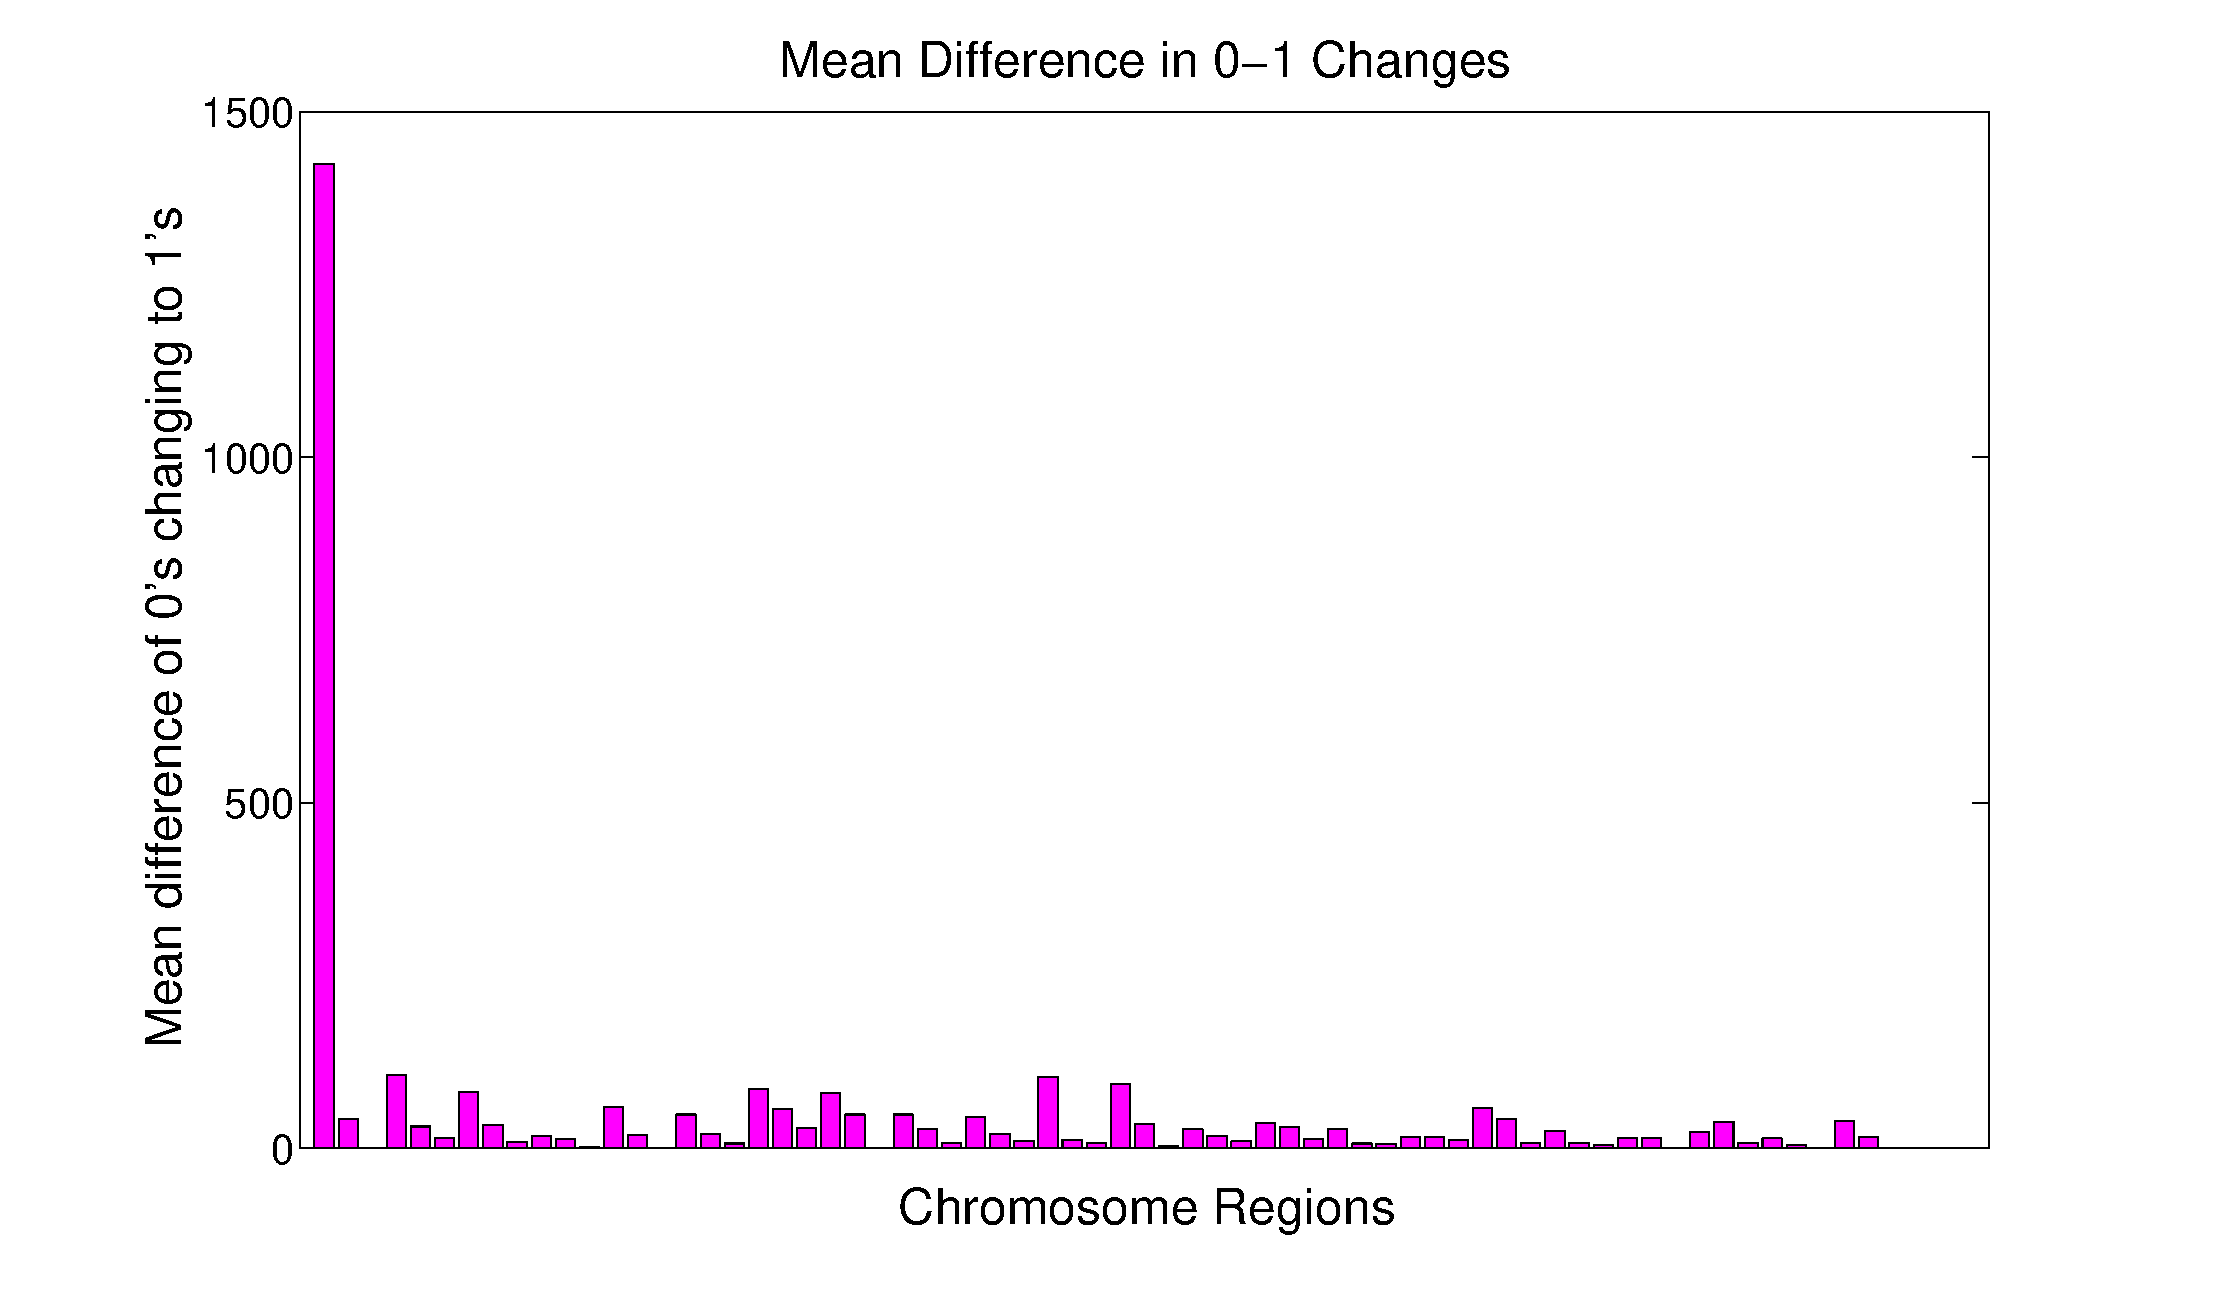
\includegraphics[width=0.9\textwidth]{figures/mean01changes1}
\caption[Differences in \mbox{0-1} Changes]{Mean of difference in number of unaberrated bands changing to aberrated bands in different downsampling methods. The X-axis varies in small intervals with respect to resolution and in larger intervals with respect to the chromosome number.} \label{Fig:0to1diff}
\end{figure}

Similar to Section~\ref{ss:totamplification}, the mean of difference between the number of the unaberrated region changing to the aberrated region was also computed and visualized with the results depicted Figure~\ref{Fig:0to1diff}. Similar to other matrices for defining the similarity/dissimilarity of the results of methods, Figure~\ref{Fig:0to1diff} shows negligible differences of cases where the unaberrated band is changed to the aberrated band in two different downsampling methods. After the results from Figure~\ref{Fig:0to1hist}, it can be inferred that some negligible differences shown in the property models discussed in Section~\ref{ss:totamplification} are the result of weighted downsampling method.

\subsection{Frequent Itemsets}
\label{ss:frequentitemsets}
Given 0-1 data, $\mathcal{D}$ with a set of attributes $\mathcal{I}_1, \mathcal{I}_2 \ldots \mathcal{I}_n $  and a support $\sigma$, a frequent set is the set  $\mathcal{F}$ of items of  $\mathcal{D}$ such that at least a fraction of $\sigma$ of the rows of $\mathcal{D}$ have 1 in all columns of $\mathcal{F}$~\cite{agrawal, apriori}. However, the major problem with frequent itemset is that if an itemset $\{ a, b, c \}$ is frequent  then their subsets are also frequent because of the anti-monotonicity property of frequent itemsets~\cite{redescription}, thus making it unsuitable for comparison and reporting. On the other hand, maximal frequent itemset can be defined as an itemset which is frequent but non of its supersets are frequent~\cite{mafia}. 

The measure of frequent itemsets also provides a metric for the similarity measure between the sampled data and original data. Furthermore, our major aim was to upsample and downsample the data so that the patterns in the original resolution were retained. Mining maximal frequent itemset in the context of the mixture modelling of multivariate Bernoulli distribution is two fold. It has been shown in~\cite{Holl20071} that maximal frequent itemset can be used to describe the finite mixture of multivariate Bernoulli distributions compactly and in a language understandable by the domain experts. In~\cite{Holl20071}, the authors implemented a mixture of Bernoulli distributions in clustering \mbox{0-1} data to derive frequent itemsets from the cluster-specific data sets and found that the cluster-specific maximal frequent itemset were significantly different from those itemsets extracted globally. 

Similar to~\cite{Holl20071}, we used MAFIA (MAximal Frequent Itemset Algorithm)~\cite{mafia} to mine the frequent patterns because other similar algorithms such as Apriori~\cite{apriori} would produce long results which will be difficult to interpret, analyze and report. The frequency or the threshold was chosen as 0.5 motivated by a majority voting protocol. Upsampling is simple and is always guaranteed to retain the frequent itemset although the number of frequent itemset increases with the exactly the same support. Therefore, they have not been reported.

\begin{table}[h!]
  \centering
  \begin{tabular}{|p{0.35\textwidth}|p{0.57\textwidth}|}
    \hline
    \textbf{Data Resolution} 	&	\textbf{Maximal frequent itemsets at threshold($\alpha$)=0.5 }\\ \hline
    Original 400 (A)		&	\{11\},\{12\}	  \\ \hline
    Original 850 (B)		&	\{7, 8, 9, 10, 11, 12, 13, 14, 15, 16, 17, 18, 19, 20, 21, 22, 23, 24\}      \\ \hline
    OR-function downsampled from B to 400 (C)		&	\{5, 6, 7, 8, 9, 10, 11, 12\}      \\ \hline
    Weighted downsampled from A to 400 (D)		&	\{7, 8\}, \{5, 6, 7\}, \{7, 12\}, \{7, 11\},  
    
    \{8, 9, 10, 11, 12\}	  \\ \hline
    Majority Decision downsampled from B to 400 (E)	&	\{5, 6, 7, 8, 9, 10, 11, 12 \}  \\ \hline
    Combined in  400 					&	\{5, 6, 7\}, \{6,7,8\}, \{7, 8, 9, 10, 11\}, 
    
    \{7, 8, 11, 12\}, \{8, 9, 10, 11, 12\}    \\ \hline
    Combined in  850 					&	\{7, 8, 9\},  \{8, 9, 10, 11, 12, 13, 14\}, \{9, 10, 11, 12, 13, 14, 15, 16, 17, 18, 19, 20, 21\}, \{9, 10, 11, 12, 13, 14, 19, 20, 21, 22, 23, 24 \}, 
    
    \{ 10, 11, 12, 13, 14, 15, 16, 17, 18, 19, 20, 21, 22, 23, 24\}      \\ \hline     
  \end{tabular}
  \caption[MFI for data in different resolutions]{Maximal frequent itemsets for data in different resolutions. The support, frequency or threshold ($\alpha$) used is 0.5. Example case for Chromosome 17.} \label{Tab:maximal}
\end{table}

From Table~\ref{Tab:maximal}, we can see that the maximal frequent itemsets are preserved during sampling of resolutions. For example, in OR-function downsampled data in resolution 400 and original data in resolution 850, there is no difference in the maximal frequent itemset because from Table~\ref{Tab:Transformation} used in upsampling,  we know that items 7, 8, and 9 in resolution 850 represents items 5, 6 and 7. Items 8 to 14 in 850 are combined to form item 8 in resolution 400. Other itemsets are also formed with similar combinations. Weighted downsampling differs more than other two types of methods but even for weighted downsampling method, the difference is not significant. The results of sampling can be seen more profoundly in integrated datasets where each itemsets in higher resolution can be defined by the frequent itemsets lower resolution. The differences in some cases are only seen because support for those itemsets are less; these differences can be expected because data in lower resolution cannot encompass all the information in higher resolution.

%\section {Summary and Conclusions}
%\label{s:conclusion}
%A simple upsampling and three different downsampling methods were proposed and their results were studied. The results were plausible and fairly consistent. The resulting data in different resolutions efficiently captures the information of data in different resolutions. Mixture models were then applied to the data in different resolutions. Finally, data in two different resolutions were integrated and then analyzed in one resolution. The results suggested that number of components required to fit the data does not differ across resolutions but likelihood of the model on higher resolution is poor than on lower resolution although the data is the same but representation is different. The clustering results of mixture models possesses high clinical significance. Furthermore, the maximal frequent itemsets and mixture modelling show that significant patterns in the data is maintained during sampling.


\subsection{Motivation for Database Integration}
\label{ss:motivationdatabseintrigation}

Two sets of original data were available in resolution 400 and 850. Experiments were performed in the original resolution and sampling was performed to sample the data to different resolutions. Data representing whole genome was divided into each chromosome. In each chromosome, the the zero vectors were removed. The cancer patients who did not exbibit chromosomal aberration in a particular chromosome were removed from the data because we were interested in modelling the chromosomal aberrations of cancer patients not their absence.
%Experiments showed that number of components required to optimally fit the model were dependent on the resolution of the data thus showing the increase in complexity with increasing dimensionality of the data. However, the observed difference were not very high, showing that the number of significant patterns were preserved during the sampling process. 

\begin{figure}[h!]
\centering
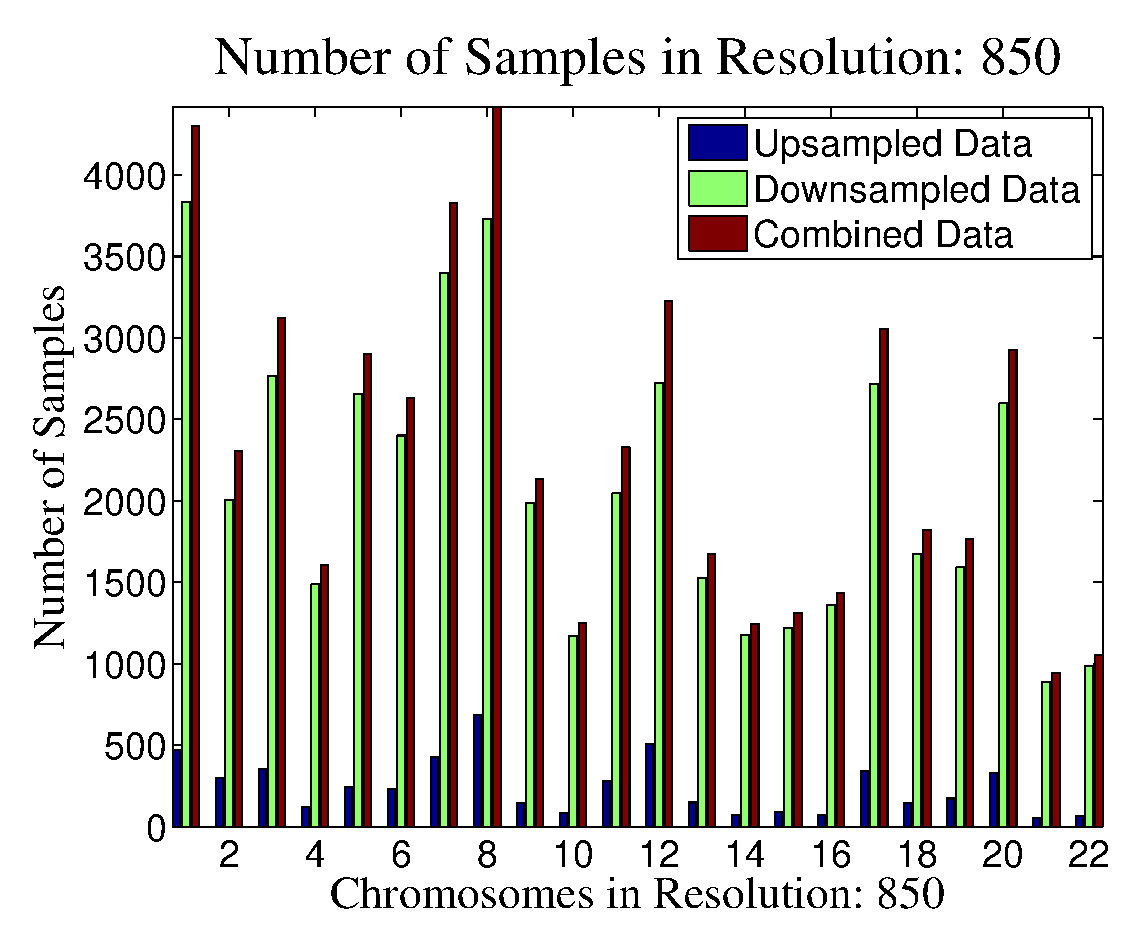
\includegraphics[width=0.95\textwidth]{figures/numsamples850}
\caption[Number of samples of data in resolution 850]{Number of samples of data in resolution 850. Figure shows the number of samples for three different datasets used for modelling in this thesis: Upsampled, Downsampled, and Combined.}\label{Fig:datasamples}
\end{figure}

Furthermore, the sample size of data reduces significantly when the data in resolution 400 is split into each chromosome and samples with all zeros i.e. zero vectors are removed. This phenomenon is captured by Figure~\ref{Fig:datasamples}. Additionally, upsampling does not increase the number of unique rows. It also shows that number of samples in upsampled data is significantly less compared to the number of samples in downsampled and combined data. 


\begin{figure}[h!]
\centering
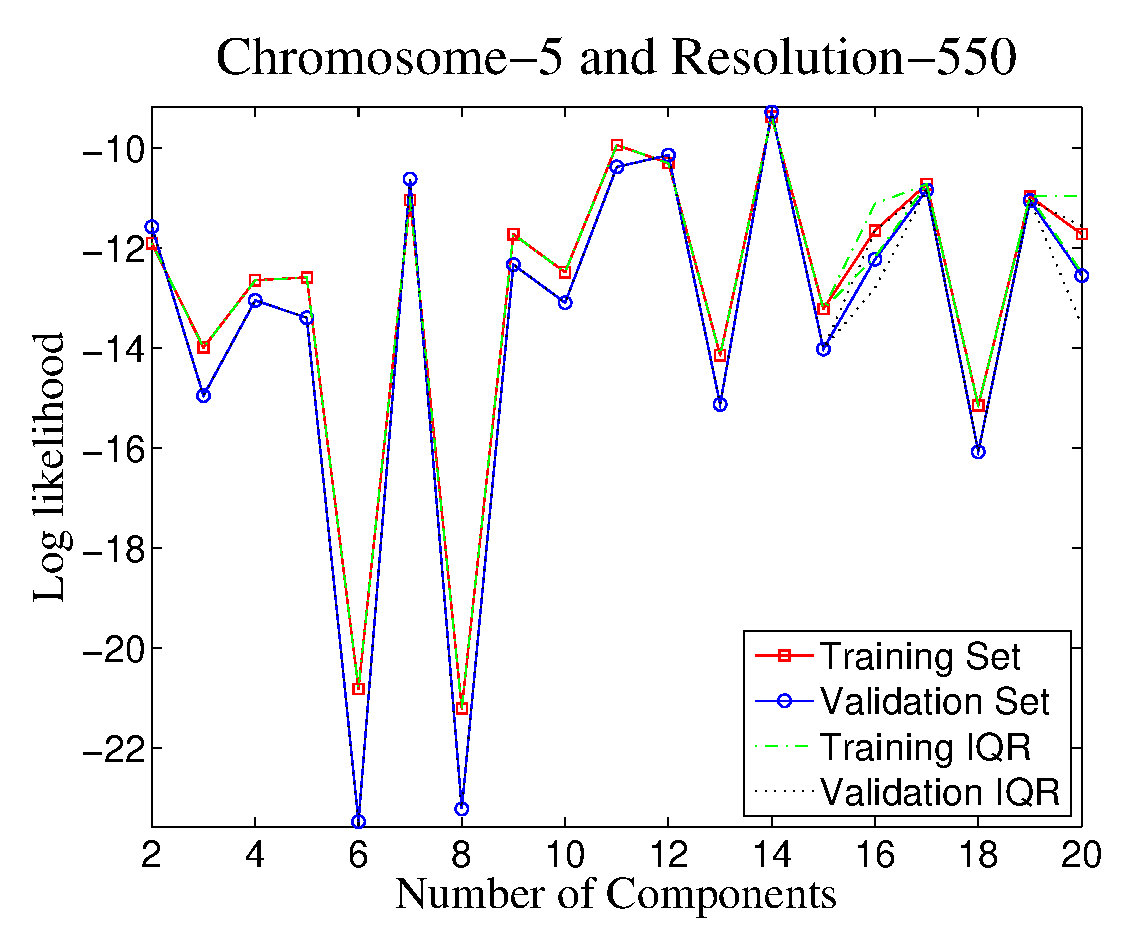
\includegraphics[width=0.9\textwidth]{figures/chr5dm550wt}
\caption[Model selection in chromosome 5 and resolution 550]{Model selection for data in resolution 550. The averaged loglikelihood for training and validation sets in a 10-fold cross-validation setting for different number of components in chromosome 5 \& Resolution 550. The interquartile range(IQR) for 50 different training and validation runs have also been plotted. The details of the model selection procedure using cross-validation is discussed in detail in Section~\ref{s:mmmbd}. This example is shown to elaborate that with few samples of data in high dimension (finer resolution) machine learning algorithms such as cross-validation does not work very well.} \label{Fig:chr5dm550}
\end{figure}

It is important to note that machine learning and data mining algorithms and methods in most cases are data hungry and require significantly large amount of data for plausible results. Thus, database integration is important to work with high dimensional data with small sample size. For example, the validation technique cross-validation used in this thesis has been shown not to work very well with small sized data samples in~\cite{unreliable, cvinmicroarray}. A simple example of cross-validation on small sample data is shown in Figure~\ref{Fig:chr5dm550} as an example case for chromosome 5 in resolution 550. Experiments with different chromosomes have shown that there is a well-defined structure present in data. The details of model selection procedure are discussed in Sections~\ref{ss:modelselection} and~\ref{ss:modelstructureselection}. Same chromosome 5 in the same resolution 550 shows the presence of definite structure in the data when the database is integrated. 

\begin{figure}[h!]
\centering
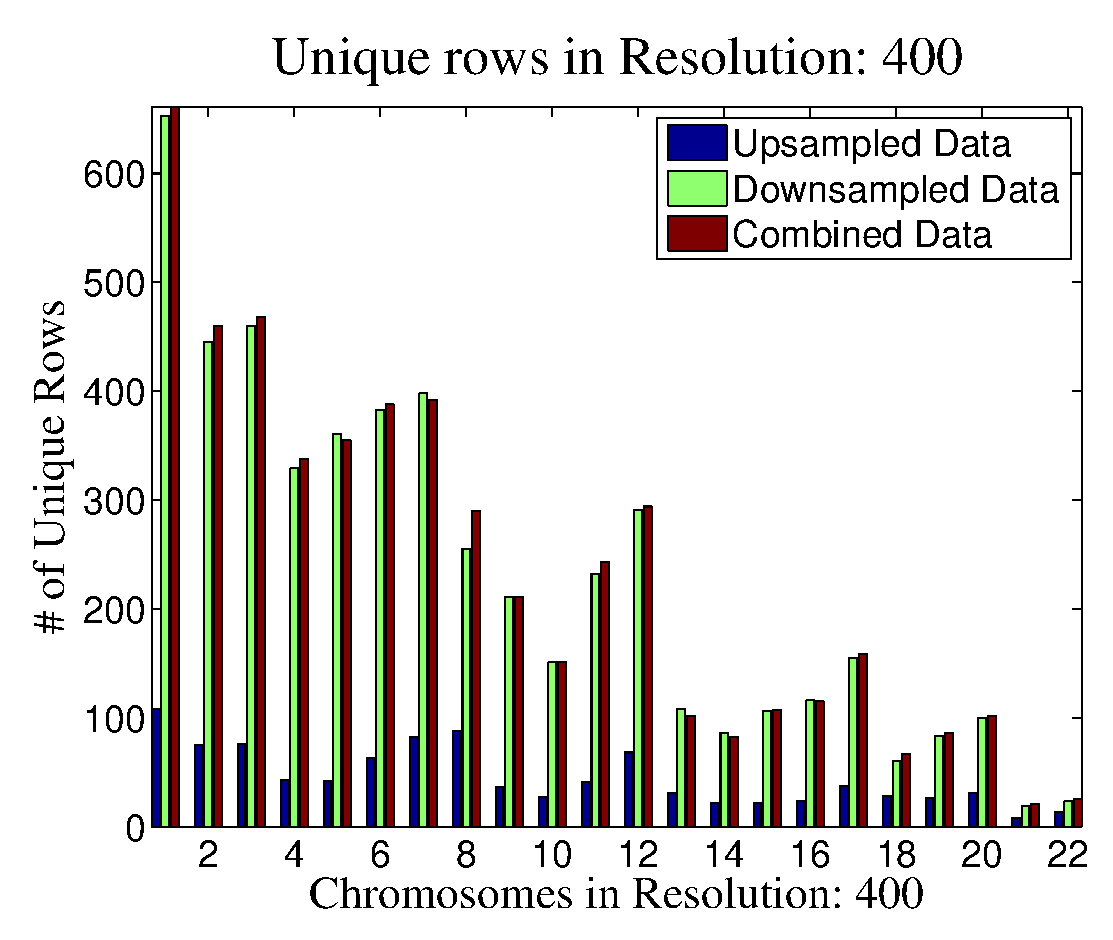
\includegraphics[width=0.95\textwidth]{figures/numunqrows400}
\caption[Number of unique samples of data in resolution 400]{Number of unique samples of data in resolution 400. Figure shows the number of unique samples of data for three different datasets used for modelling in this thesis: Upsampled, Downsampled, and Combined.}\label{Fig:ratioschr}
\end{figure}

Unlike many real valued data, the size of the \mbox{0-1} data seems to be significantly large, often large datasets are turned to \mbox{0-1} data for the ease of analysis. For instance, consider the size of some of the benchmark datasets: RETAIL \cite{retail} is 200000 by 20000; KOSARAK is 100000 by 40000 as described and preprocessed in \cite{randomization}. One important issue to note is that the main property of the \mbox{0-1} data is their large dimension. However, dataset at our disposal was relatively small and the problem was further compounded by the presence of few unique rows thus making database integration inevitable.

In general 0-1 datasets, even when the data set is large, ratio of unique rows to the number of samples in the dataset is also approximately 1 i.e. all of the rows in the data are unique. Figure \ref{Fig:ratioschr} shows the number of unique rows for the dataset used in the experiments consisting of 22 chromosomes in 4 different resolutions. Figure \ref{Fig:ratioschr} shows that unlike the other \mbox{0-1} dataset, the dataset used in the experiments has very few unique rows. Furthermore, the number of copies of unique rows are not evenly distributed. Additionally, the amplification data is more skewed and sparse. For example, element-wise AND operation between elements in the same column results in zero vector. Thus, in this setting, with a very few samples of data, cross-validation can always suffer from the problem of ``\texttt{unfortunate split}''\footnote{For example, in a classification problem, if certain class is not represented by training set, then the model is not trained to classify it thus producing poor results on the future data.}. When database is integrated, the number of samples in the dataset increases also increasing the number of unique samples in the dataset. Thus, experiments were performed after primarily combining the datasets in different resolutions as well as two different resolutions independently in order to compare the results.

\section{Mixture Modelling of Multivariate Bernoulli Distributions}
\label{s:mmmbd}
\subsection{Model Selection}
\label{ss:modelselection}
Model selection is a process of selecting the best model from a set of possible models that optimally fit the data. It is one of the most challenging tasks in machine learning and there are no well defined rules to select the best model and this is an ``unsolved'' problem in statistics. Often, model selection depends on the use of some prior information, especially about the data, and `\textit{the rule of thumb}'\footnote{Definition from Merriam-Webster Online Dictionary: Rule of thumb - a general principle regarded as roughly correct but not intended to be scientifically accurate.}. In other words, the model selection itself can be regarded as ``Data Mining''. A simple prototyping of models and their statistical analysis can be used to select the model. However, such process will be highly cumbersome. For example, given a machine learning problem, it is very difficult, if not impossible to select the best method from a myriad of the machine learning method such as Support Vector Machines~\cite{svm, svm1}, Multilayer Perceptions~\cite{hykin, perceptron}, Extreme Learning Machine~\cite{elm}, among many others.  In this thesis, the problem was to analyze copy number aberrations data relevant to cancer. Cancer is not a single disease but a heterogeneous collection of several diseases. We decided to work in the probabilistic context and decided to model the data using a model that possesses clustering capabilities. Furthermore, cancer is a multifactorial disease. Therefore, mixture modelling was selected to model the copy number aberrations data because they provide an efficient method of modelling the heterogeneous population. Furthermore, since the copy number aberrations data was a high dimensional \mbox{0-1} data, the distribution used in the mixture model is the Bernoulli distribution. However, mixture models are too complex in bigger dimension in terms of both time and space complexity. Furthermore, the chromosomal aberrations dataset analyzed in this thesis uses very scarce data as explained in Section~\ref{s:dataset}. Thus, we decided to work  chromosomewise because of the availability of very few samples of the data to constrain the complexity of the mixture models. 


\subsection{Model Structure Selection}
\label{ss:modelstructureselection}
After the selection of the model, the solution of one difficult problem is accomplished but another one awaits which is the problem of model structure selection. The model structure selection is the application of statistical methods for selecting the parameters and hyperparameters of the model. For example, given a machine learning problem, we choose to model it with polynomial curve fitting assuming some prior knowledge that the model is not linear. Even in polynomial curve fitting: the choice among $ax+b$, $ax^2+bx+c$ and other higher order polynomials is an arduous task. The concept of underfitting, overfitting, bias-variance dilemma (trade-off) are the central issues to be considered in model structure selection. These are very important concepts in machine learning but the thesis does not consider the details of these methods. The details of these concepts can be acquired from Sections 6.1, 9.1 of~\cite{bishop}; Sections 6.8, 6.9 of~\cite{gruney}; and Sections 2.13, 4.13 of~\cite{hykin}. In this thesis, the model selected is mixture models. The hyperparameters of mixture models are the number of mixture components~\cite{componentdet}. Therefore, the model structure selection problem in this thesis is restricted to the selection of number of mixture components in the mixture model.

The size of the chromosome in terms of number chromosome bands and also the number of samples varied significantly which are tabulated in Table~\ref{Tab:chrsub}. Some chromosomes had greater number of bands and some chromosomes had lower number of chromosome bands. Data from different resolutions were individually subjected to the mixture models. The central problem in this case is model selection which is to determine the number of components in the mixture model. We used the 10-fold cross-validation approach to train the model of different complexities. The exercise was repeated 50 times i.e. for each mixture component, 50 models were trained using training set and their performance was evaluated on the test set. It is often recommended to repeat cross-validation technique a number of times because 10-fold cross-validation can be seen as a ``standard'' measure of the performance whereas ten 10-fold cross-validations would be a ``precise'' measure of performance~\cite{kayphdthesis}. Since EM algorithm is sensitive to the initializations and the results may differ on the same data for different initializations and it can susceptible local minima and the global optimum results are not often guaranteed~\cite{embook}, 50 different models were trained for each number of components. The number of mixture components was varied from 2 to 20 for all chromosomes in all resolutions. The assumption here is that each chromosome has at least two clusters and more than 20 clusters overfits the data for each chromosome where the maximum dimensionality of the data was 63. Validation set for each model is the one remaining subset of the data which is not used for training. Total likelihood for the training data as well as the validation data is calculated and averaged for each mixture component. We select the model that is able to produce better generalization capabilities (i.e. the number of components for which the likelihood is maximum) taking parsimony into account. In other words, in some cases, models with lesser mixture components are selected instead of models with the larger number of mixture components for which likelihood was higher. We also calculate Interquartile Range(IQR) for training and validation likelihood to analyze the statistical dispersion of the likelihood in different models for the same number of components. Components, for which the variation in IQR is high or which shows more dispersion, are not reliable and hence avoided in most cases. Model selection was performed on all chromosomes as chromosomewise analysis can reveal interesting facts about the aberrations of specific chromosomes and guarantees efficient computation \& ease of analysis. Figures~\ref{Fig:chr17dm393} and~\ref{Fig:chr17dm850} show model selection procedure for the data in resolution 400 and 850 respectively.

\begin{figure}[h!]
\centering
\includegraphics[width=0.95\textwidth]{figures/chr17dm400lat}
\caption[Model selection in chromosome 17 and resolution 400]{Model selection for the the original data in resolution 400. The averaged loglikelihood for training and validation sets in a 10-fold cross-validation setting for different number of components in chromosome 17 \& Resolution 400. The interquartile range(IQR) for 50 different training and validation runs have also been plotted. Here, number of components (J) selected is 6.}\label{Fig:chr17dm393}
\end{figure}

The figure also shows the model selection in case of resolution 400 which downsampled from resolution 850. Figure~\ref{Fig:chr17dm393} shows that the likelihood is smoothly increasing function with respect to the number of components. From Figure~\ref{Fig:chr17dm393}, it can be seen that validation likelihood is maximum when the number of components is 12, but instead of 12 components, 6 components was selected. It is to be noted that sometimes complex models overfit the data and the simple models reduce the time and space complexity. Furthermore, the training and validation likelihood when the number of components is 6 are -3.5293 and -4.0666. In addition, when the number of components is 12, the training and validation likelihood are -3.0972 and -3.8956. Hence, the difference in likelihood is negligible when compared with the efficiency in terms of time and space complexity. Furthermore, when the number of components is increased, IQR(Inter Quartile Range) shows significant variation. The variation in IQR is because when the number of components is increased, samples can be assigned to different clusters in different runs of the k-fold cross-validation. Additionally, the data in resolution in 400 was upsampled to resolution 850 and similar approach to select the model was followed. 

\begin{figure}[h!]
\centering
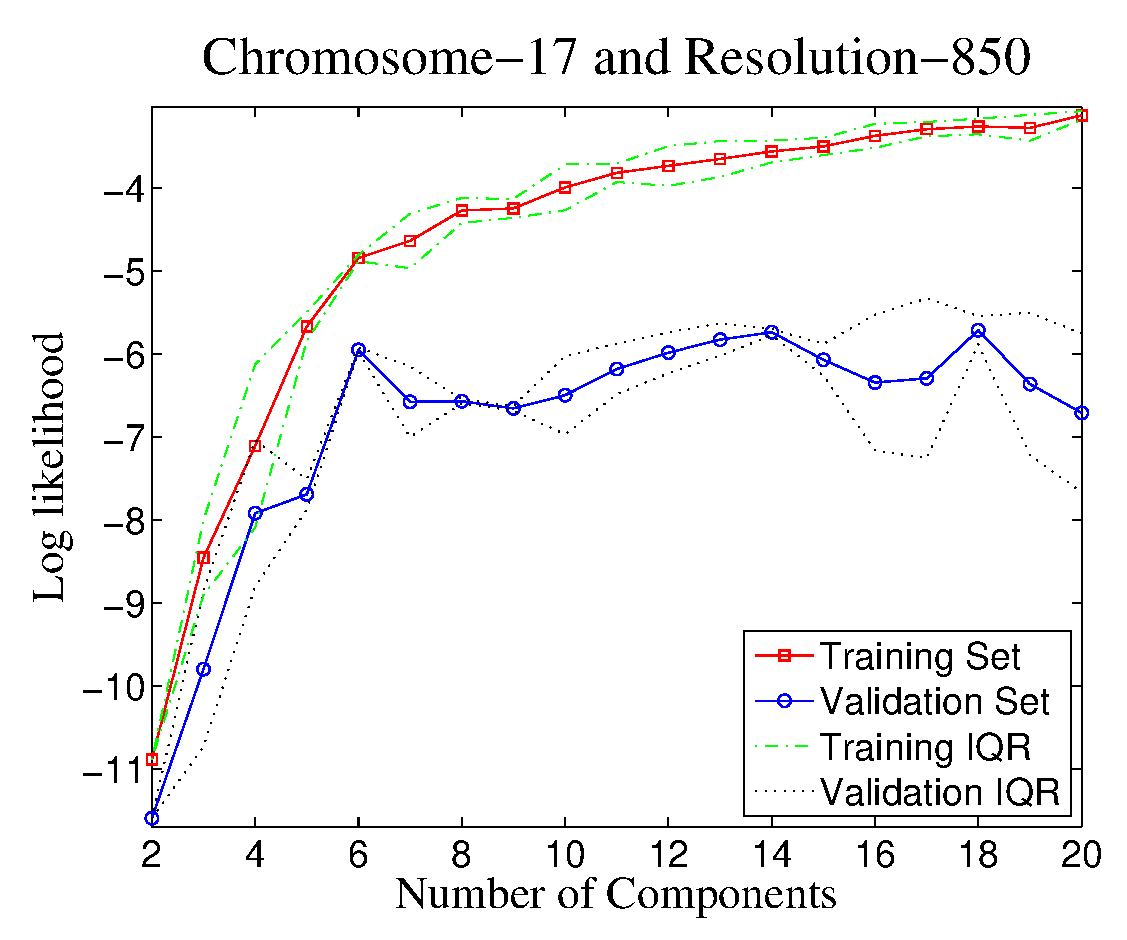
\includegraphics[width=0.95\textwidth]{figures/chr17dm850lat}
\caption[Model selection in chromosome 17 and resolution 850]{The averaged loglikelihood for training and validation sets in a 10-fold Cross-validation setting for different number of components in chromosome 17 and resolution 850. The interquartile range(IQR) for 10 different training and validation runs have also been plotted. Here, number of components (J) selected is 6.} \label{Fig:chr17dm850}
\end{figure}

Figure~\ref{Fig:chr17dm850} also shows that the IQR varies significantly from the mean likelihood. The choice of the number of components is straightforward  because Figure~\ref{Fig:chr17dm850} clearly shows a maximum of validation likelihood when the number of components is 6. Even when the number of components is 6, the variation in IQR is also low. However, the variation in IQR can be compensated with sufficient training which would produce favorable results. Thus, we train different models and select the best one among them as discussed in Section~\ref{ss:parameterestimation}. The results can be further improved when the size of the dataset is increased which motivates our upsampling and downsampling strategies for database integration.

\subsubsection{Parameter Estimation}
\label{ss:parameterestimation}
After the selection of model and its hyperparameters are performed, the parameter estimation is relatively a simple task. Parameter estimation is also often referred to as model fitting, model training or model learning in machine learning literature~\cite{bishop, mitchell}. Consider, for example, in the above case of polynomial curve fitting, assume that we selected the model is $ax+b$. Now, the value of $a$ and $b$ can be optimized or learned from the data. 

 \begin{figure}[h!]
 \centering
 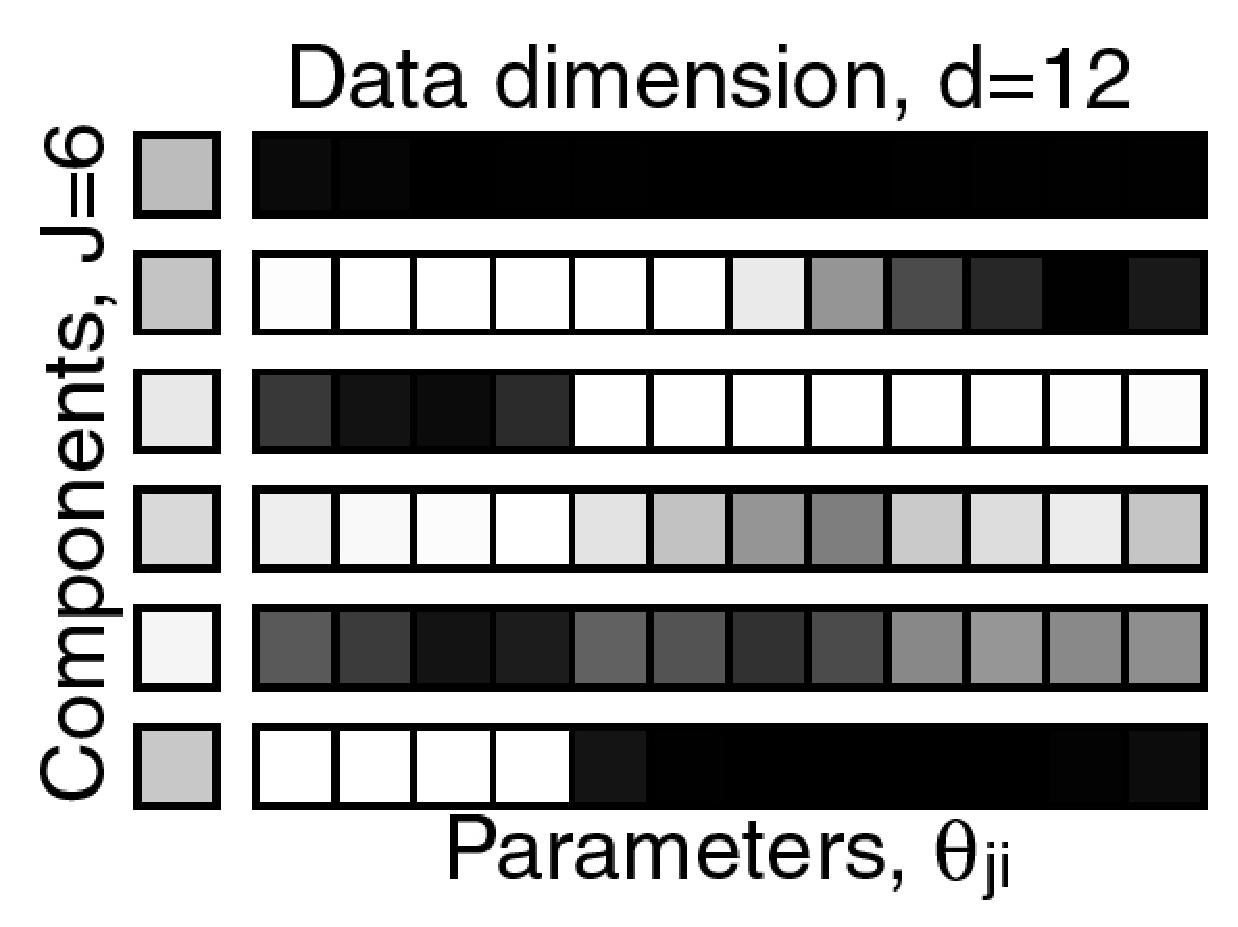
\includegraphics[width=0.8\textwidth]{figures/mdlchr17dm393}
 \caption[Final Trained Model in chromosome 17 and resolution 400]{Visualization of one of the trained models for chromosome 17 in resolution 400 for combined data. Here the selected number of components is 6 which corresponds to the rows in the model. The first separate column determine the mixing proportions of each mixture component. The remaining 12 columns determines the parameters $\theta_{ji}$. Darker colors denotes the higher values of the parameters.}\label{Fig:mdl1}
 \end{figure}

In this thesis, after the number of components are selected, the model is trained with all the available data to determine the optimal value of the Bernoulli parameter $\theta$ using EM algorithm~\cite{wolfe, everittmixdist}. In order to achieve the best results  while finally selecting the model after selecting the number of components, we further train 50 different models of the same complexity (i.e. the same number of components) to convergence and select the best model in terms of the likelihood produced on the original data. The value of $\theta$ specify the probability that a random variable takes the value 0 or 1. 


 \begin{figure}[h!]
 \centering
 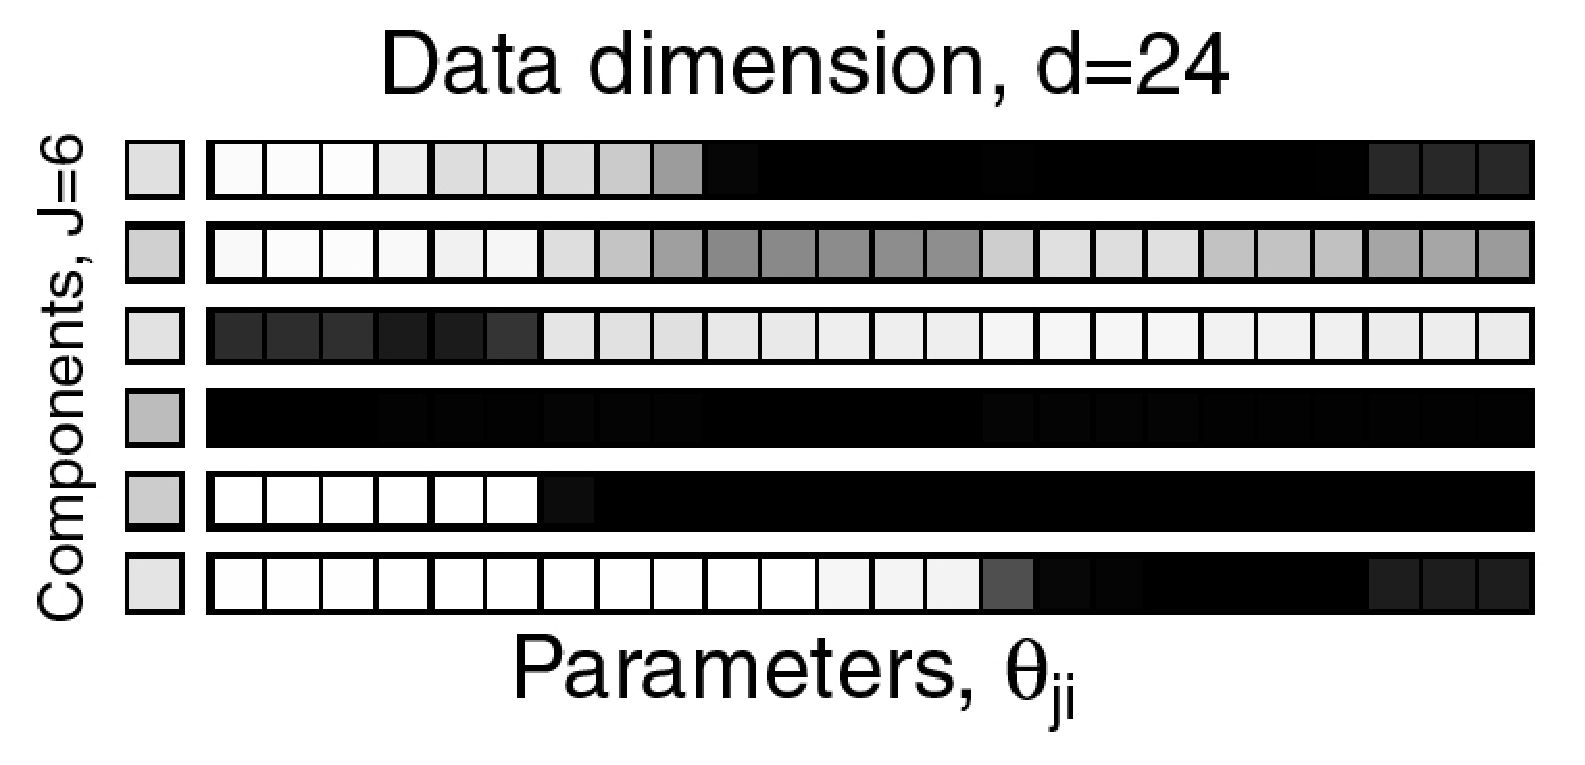
\includegraphics[width=0.95\textwidth]{figures/mdlchr17dm850}
 \caption[Final Trained Model in chromosome 17 and resolution 850]{Visualization of one of the trained models for chromosome 17 in resolution 850 for combined data. Here the selected number of components is 6 which corresponds to the rows in the model. The first separate column determines the mixing proportions of each mixture component. The remaining 24 columns determine the parameters $\theta_{ji}$. Darker colors denotes the higher values of the parameters.}\label{Fig:mdl2}
 \end{figure}

The best of the trained models are used to calculate the likelihood on data as shown Table~\ref{Tab:results}. The model was also used to sample the data to be used in validation using resampling approach as discussed in Section~\ref{ss:resampling}. Figures~\ref{Fig:mdl1} and~\ref{Fig:mdl2} are the final models trained to convergence for combined data in resolution 400 and 850 respectively. Similarity of the models can be tracked visually from the model visualization as in Figures~\ref{Fig:mdl1}~and~\ref{Fig:mdl2}. For example, Component~6 in Figure~\ref{Fig:mdl1} corresponds to Component~1 in~\ref{Fig:mdl2}. Similarly, Component~1 in Figure~\ref{Fig:mdl1} corresponds to Component~4 in Figure~\ref{Fig:mdl2}.
 
 \subsection{Computational Complexity}
 \label{ss:compcomplex}
 \begin{table}[h!]
  \centering
  \begin{tabular}{|l|c|c|c|}
    \hline
%    \multicolumn{4}{|c|}{\textbf{Chromosome 1}}\\   \hline 
%    \multirow{2}{*}{\textbf{Data Resolution}} & \multirow{2}{*}{\textbf{\# of Samples}} &  \multicolumn{2}{|c|}{\textbf{Time in Seconds}} \\ \cline{3-4}   
% 			&		&\textbf{Training} & \textbf{Testing} \\ \hline   
%     Original in 400	&		& 	& 	\\ \hline
%     Original in 850	&		& 	& 	\\ \hline
%     Downsampled to 400	&		& 	& 	\\ \hline
%     Upsampled to 850	&		& 	& 	\\ \hline
%     Combined in 400	&		& 	& 	\\ \hline
%     Combined in 850	&		& 	& 	\\ \hline  
%     
    \multicolumn{4}{|c|}{\textbf{Chromosome 17}}\\   \hline 
    \multirow{2}{*}{\textbf{Data Resolution}} & \multirow{2}{*}{\textbf{\# of Samples}} &  \multicolumn{2}{|c|}{\textbf{Time in Seconds}} \\ \cline{3-4}   
				&		&\textbf{Training} & \textbf{Testing} \\ \hline   
    Original in 400(A)		&	342	& 0.25	  & 0.06	\\ \hline
    Original in 850(B)		&	2716    & 0.43    & 0.30	\\ \hline
    Downsampled to 400 from B(C)&	2716    & 1.12	  & 0.20	\\ \hline
    Upsampled to 850 from A(D)	&	342	& 2.16	  & 0.08	\\ \hline
    Combined in 400(A+C)	&	3058    & 1.43    & 0.19	\\ \hline
    Combined in 850(B+D)	&	3058    & 2.51    & 0.32	\\ \hline  
  \end{tabular}
  \caption[Computational complexity of mixture models]{Computational complexity for training and testing of a single mixture model with appropriate number of mixture components as decided in Table~\ref{Tab:results}. Experiments are performed on chromosome 17 and time is calculated in seconds. X denotes the number of data samples. The hardware used is Intel Core2Duo 2.00GHz CPU with a memory of 3 GB.}\label{Tab:computation}
\end{table}

The major drawback in using mixture models is the computational complexity of training the mixture models. Normally, training mixture models are computationally expensive when compared with other parametric (such as Poisson distribution~\cite{poission}) as well as non-parametric (such as k-means~\cite{kmeans, kmeans2}) methods. Similar to other machine learning methods, computational complexity of the mixture model also increases with increasing dimension which is determined by resolution in our case. Thus, computational complexity was also estimated for each resolution for the selected number of components. As shown in the Table~\ref{Tab:computation}, the computational complexity increases in the fine resolution. To estimate the training time, fifty different models are trained until ten iterations and the mean of the result is taken as final training time. Similarly, likelihood is calculated for fifty different models trained to calculate the training time and the mean of the results is reported. Experiments with resolution 850 required approximately twice the time required for resolution 400. Furthermore, from Table~\ref{Tab:results}, we also know that number of components required is high when the resolution is increased but the likelihood decreases. In addition, the curves are smoother in Figure~\ref{Fig:chr17dm393} compared with Figure~\ref{Fig:chr17dm850}. This phenomenon is because of the intrinsic problems of working with high dimensional data arising in fine resolution, the phenomenon is often referred to as the `\textit{curse of dimensionality}'~\cite{curse}. These results suggest that data in lower resolution is preferred but lower resolution does not capture all the available biological information. Thus, there is a trade-off between the two.

\subsection{Experimental Design}
\label{ss:experimentalprocedure}

\begin{figure}[h!]
\centering
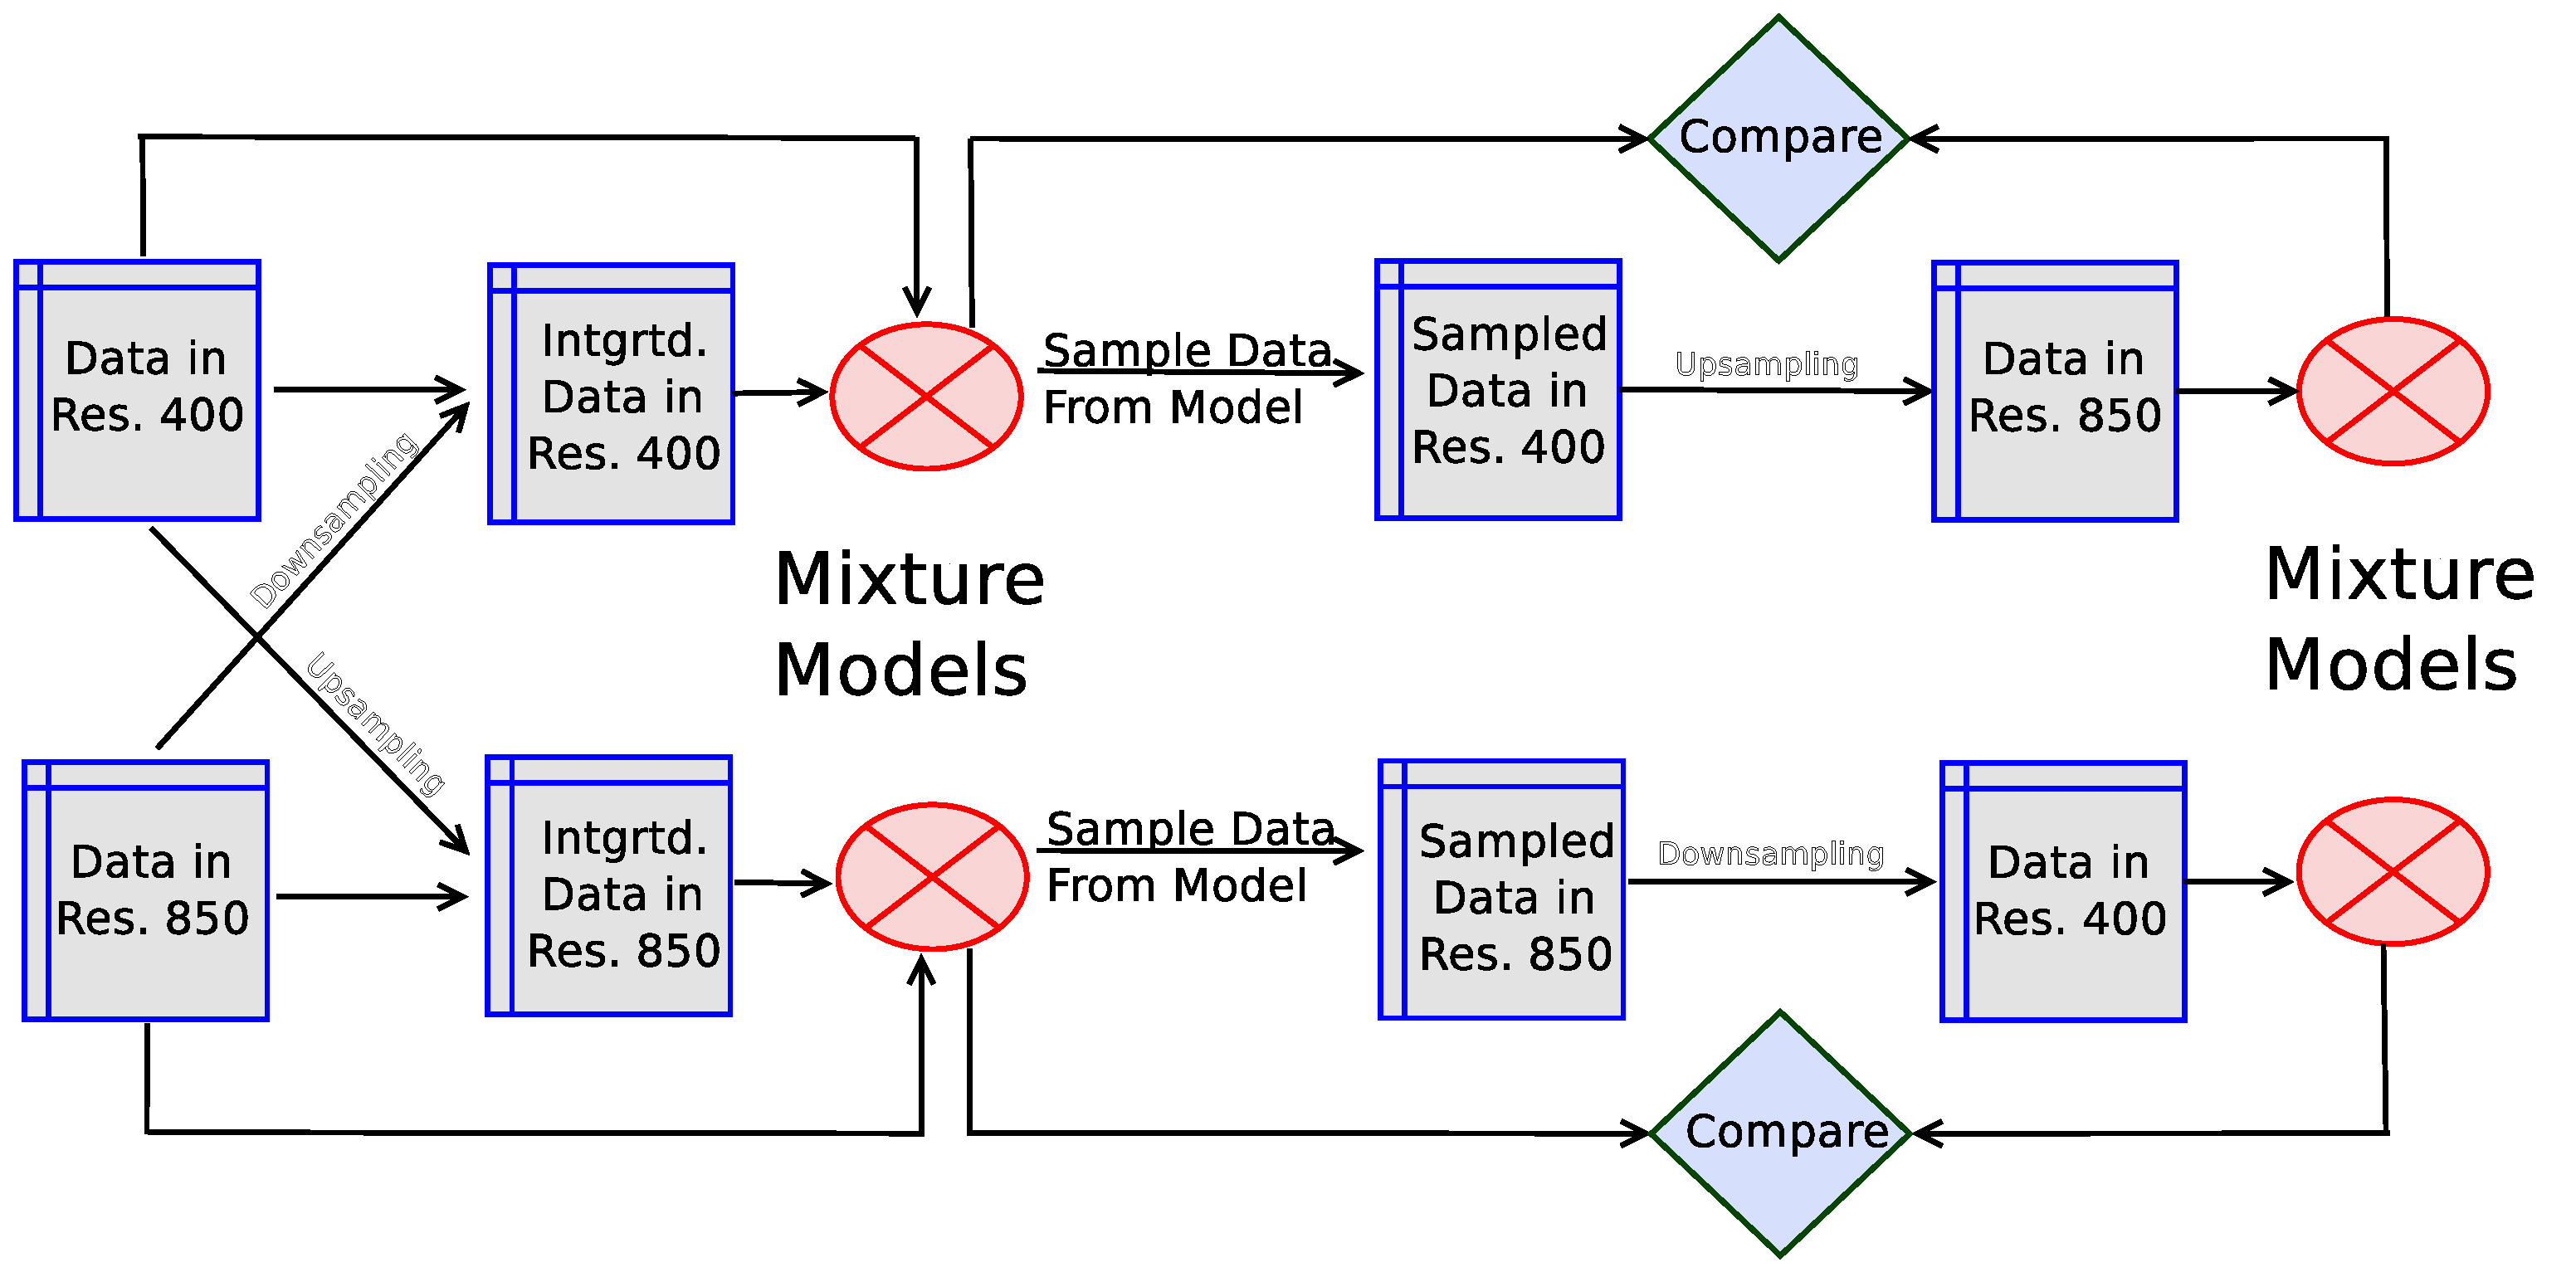
\includegraphics[width=0.95\textwidth]{figures/process}
\caption[Experimental procedure]{The overall experimental procedure in this thesis.}\label{Fig:expmproc}
\end{figure}

Experimental procedure is as depicted in Figure~\ref{Fig:expmproc} shows that there are two sets of data in two different resolutions: 400 and 850. We use upsampling and downsampling to integrate the data. We then model the data using mixture models. We also model the data individually without integration so that we can compare the results when the database is integrated. We use 10-fold cross-validation repeated fifty times to select the number of components in the mixture model. After selecting the number of components, fifty different models were trained to convergence and best of the trained models in terms of likelihood is taken as the final model for the data. Since the mixture models are generative models, we sample the data from the trained mixture models. We then than use the same model selection approach to the sampled data after upsampling and downsampling so that we can compare the results. We also compare frequent patterns in the original and the sampled data to evaluate whether our sampling and modelling effort has preserved the overall structure in the data as well as the frequent patterns in the data. 
 
\subsection{Results}
The major aim of upsampling and downsampling was to aid in the integration of databases. The clinical aspects regarding the classification of cancer with mixture models is already established in~\cite{Myllykangas200815} and \cite{Myllykangas20067324}. Thus, data in different resolution are integrated after upsampling and downsampling and model selection was performed. Table~\ref{Tab:results} summarizes the results of the experiments on chromosome 17 in different resolutions. To calculate the Likelihood 50 different models were trained to convergence and likelihood of the data was calculated for each model and the mean of the results are reported.

\begin{table}[h!]
  \centering
  \begin{tabular}{|l|c|c|}
    \hline
    \textbf{Data Resolution} & \textbf{Components (J)} &\textbf{Likelihood}  \\
    \hline
    Original in 400(A)		&	6	& 	-3.39  \\ \hline
    Original in 850(B)		&	8	& 	-4.53  \\ \hline
    Downsampled to 400 from B(C)&	7	& 	-3.27  \\ \hline
    Upsampled to 850 from A(D)	&	8	& 	-4.31  \\ \hline
    Combined  in 400(A+C)	&	6	& 	-3.48  \\ \hline
    Combined in 850(B+D)	&	6	& 	-5.20  \\ \hline     
  \end{tabular}
  \caption[Results on Chromosome 17 in original data]{Results of experiments on chromosome 17 in different resolutions showing the number of components required to fit the data along with their respective likelihood. The results for other chromosomes are summarized in Appendix~\ref{ap:appendRslt}.}\label{Tab:results}
\end{table}

Table~\ref{Tab:results} shows the number of components required to fit the data differs in different resolution. The likelihood of data in fine resolution is lower than the likelihood of the data in the coarse resolution when the number of components are the same. This phenomenon can be attributed to the curse of dimensionality~\cite{curse}. For example, the dimensionality of data in resolution 400 and 850 differs by 12 in chromosome 17 but likelihood is lesser even when the number of components is equal. For the original data in resolution 400 and 850, the difference in number of parameters of the model is ${6*(1+26)}-{6*(1+18)}=48$ which invites significant amount of computational complexity. The increased complexity however does not produce corresponding the increase in the likelihood. With increasing samples, the number of components is not increased because the complexity of mixture models depends on the complexity of the problem being solved, not with the size of dataset. Table \ref{Tab:finalresults} summarizes the final results of the experiments in all chromosomes. 


\begin{table}[h!]
  \centering
\begin{tabular}{|c|c|c|c|r|r|r|}\hline
\multicolumn{7}{|c|}{\textbf{Upsampled Data}} \\ \hline
\multirow{2}{*}{\textbf{Resolution}} & \multicolumn{3}{|c|}{\textbf{\# of Components}} &  \multicolumn{3}{|c|}{\textbf{Log Likelihood}} \\ \cline{2-7}
    & $Mean$ & $Mode$ & $Std.$ $Dev.$  & $Mean$ & $Mode$ & $Std.$ $Dev.$   \\ \hline
400 & 5.1363 & 4 & 1.3200 & -4.1170 & -6.8321 & 1.3194  \\ \hline
550 & 5.8181 & 5 & 1.4354 & -5.6478 & -12.925 & 3.3085  \\ \hline
700 & 5.6818 & 5 & 1.6442 & -9.3383 & -21.0159 &  5.6227  \\ \hline
850 & 6.4091 & 8 & 1.8685 & -10.2319 & -20.7890 &  6.2510  \\ \hline
\multicolumn{7}{|c|}{\textbf{Downsampled Data}} \\ \hline
\multirow{2}{*}{\textbf{Resolution}} & \multicolumn{3}{|c|}{\textbf{\# of Components}} &  \multicolumn{3}{|c|}{\textbf{Log Likelihood}} \\ \cline{2-7}
    & $Mean$ & $Mode$ & $Std.$ $Dev.$  & $Mean$ & $Mode$ & $Std.$ $Dev.$   \\ \hline
400 & 6.1818 & 7 & 0.9579 & -4.3354 & -8.0169  &  1.7914  \\ \hline
550 & 6.8181 & 7 & 1.1396 & -5.4993 & -11.7850 &  2.8190  \\ \hline
700 & 6.8181 & 7 & 0.9579 & -7.2905 & -13.4629 &  3.8663  \\ \hline
850 & 7.0000 & 6 & 1.2344 & -8.1149 & -15.0200 &  4.0383 \\ \hline
\multicolumn{7}{|c|}{\textbf{Combined Data}} \\ \hline
\multirow{2}{*}{\textbf{Resolution}} & \multicolumn{3}{|c|}{\textbf{\# of Components}} &  \multicolumn{3}{|c|}{\textbf{Log Likelihood}} \\ \cline{2-7}
    & $Mean$ & $Mode$ & $Std.$ $Dev.$  & $Mean$ & $Mode$ & $Std.$ $Dev.$   \\ \hline
400 & 6.2272 & 6 & 1.1097 & -4.3801 & -8.1897  & 1.7546  \\ \hline
550 & 6.6818 & 6 & 1.1291 & -5.6528 & -11.6969 & 2.8333  \\ \hline
700 & 6.6818 & 7 & 1.0413 & -7.6022 & -13.4560 & 4.0573  \\ \hline
850 & 6.8181 & 7 & 1.1396 & -8.3920 & -16.5590 & 4.2943  \\ \hline
\end{tabular}
\caption[Summary of Results on all chromosomes]{ Summary of results of experiments on all showing the number of components required to fit the data along with their respective likelihood. Here $Std.$ $Dev.$ is the standard deviation ($\sigma$.) The details of the results each chromosome are tabulated in Appendix~\ref{ap:appendRslt}.} \label{Tab:finalresults}
\end{table}

Table~\ref{Tab:finalresults} shows that the number of components selected for the data is highly co-related with the data resolution: the finer the resolution the higher the number of components required. Increasing resolutions require more number of components and the likelihood of the data also decreases. This phenomenon can be attributed to the curse of dimensionality~\cite{curse}. The difference in likelihood showing poorer fit to the data is clearly captured by the increasing standard deviation ($\sigma$) where in each of the three cases of three different datasets, the standard deviation for the likelihood increases significantly. There is only small differences in selection of number of components where as there is a significant difference in the likelihood of the final model. This behavior can also be attributed to the fact that the models selected in our case were parsimonious models. The models of higher complexity were not selected even if it produced higher validation likelihood for the fear of overfitting and computational \& space complexity of complex models. Especially models of complexity greater than ten were discarded. Furthermore, similarity in the number of components also shows that mixture models learns the structure of data relatively well although it is constrained by the increasing dimensionality of the data in finer resolution.

\begin{figure}[h!]
\centering
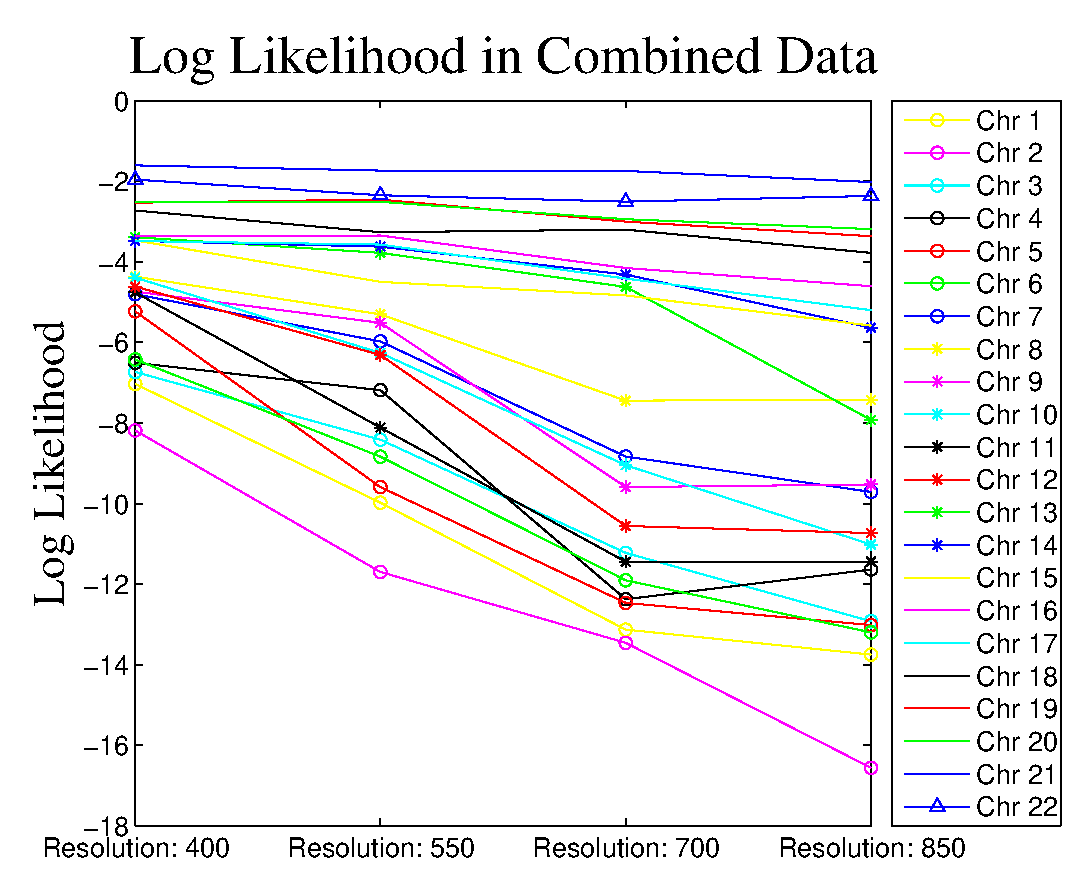
\includegraphics[width=0.95\textwidth]{figures/parcorcombined}
\caption[Parallel co-ordinates plot of likelihood of integrated data]{Parallel co-ordinates plot for the likelihood of combined data of 22 different chromosomes in 4 different resolutions.}\label{Fig:parcorcombined}
\end{figure}

In order to capture the notion of decreasing number the likelihood of data in 22 different chromosomes in 4 different resolutions, we plot the parallel co-ordinates of the log-likelihood in all three datasets: upsampled, downsampled, and combined. The plots for the three cases are similar, therefore, only the plot for combined data has been shown in Figure~\ref{Fig:parcorcombined}. The trend of decreasing likelihood can be easily captured from Figure~\ref{Fig:parcorcombined}. In few cases, such as chromosome 22 and other small chromosomes\footnote{The chromosomes are numbered by their size with only one exception i.e. chromosome 21 is smallest instead of chromosome 22. Thus, chromosome 21 is smallest chromosome while chromosome 1 is the largest of the chromosomes.}, the trend in decrease is not significant because the difference in number of chromosome bands (regions) is negligible in the smaller chromosomes. 


The computational complexity increases in the finer resolution. Moreover, high-resolution data incorporates significant amount of noise thus producing explosion of redundant patterns thus requiring more number of components to optimally fit the data. The problem with such redundant patterns can be remedied by downsampling the data if the information loss is insignificant during downsampling.


\subsection{Validation Using Data Resampling approach}
\label{ss:resampling}

\begin{figure}[h!]
\centering
\includegraphics[width=0.95\textwidth]{figures/chr17dm400resample}
\caption[Model selection in resampled data]{The averaged loglikelihood for training and validation sets in a 10-fold Cross-validation setting for different number of components in chromosome 17 and resolution 400 in resampled data from the model of combined data. The interquartile range(IQR) for 10 different training and validation runs have also been plotted. The number of components selected here is 6. }\label{Fig:sampmdlsel}
\end{figure}

This experiments with the mixture models also show that patterns present in the fine resolution of the data are efficiently and effectively preserved in coarse resolution.  Since the mixture models are generative models, we can sample the data from the trained models. Thus, in order to validate the model and determine if it has been able to extract the original structure in the data, we sample the data where the number of samples in the sampled data are equal to the number of samples used in training. We repeat the same model selection procedure as discussed in Section~\ref{s:mmmbd}. It has been shown in~\cite{premprib} that the generative mixture models preserves the statistically significant patterns in multiresolution \mbox{0-1} data. From Figure~\ref{Fig:sampmdlsel}, we can see that the number of selected components distributions are similar to the original data including the variations in the likelihood with increasing number of components. However, as expected the curve is more smooth. As with all the other experimental procedure, this validation using the data resampling approach was performed in all the chromosomes. There were very few discrepancies which occurred especially  in upsampled data. The reason being that there were very few samples of the data in upsampling. We further train the mixture model on the resampled data using the selected number of components. The model trained on the resampled data is also used to calculate the likelihood on the original data. 

 \begin{table}
  \centering
  \begin{tabular}{|l|c|c|c|}
    \hline
    \multirow{2}{*}{\textbf{Data Resolution}} & \multirow{2}{*}{\textbf{$J$}} &  \multicolumn{2}{|c|}{\textbf{Likelihood in}} \\ \cline{3-4}   
				& 	&\textbf{Original} & \textbf{Resampled} \\ \hline   
    Original in 400(A)		& 6	& -3.70	& -3.32	\\ \hline
    Original in 850(B)		& 8	& -4.57	& -4.66	\\ \hline
    Downsampled to 400 from B(C)& 7	& -3.28	& -3.26	\\ \hline
    Upsampled to 850 from A(D)	& 8	& -4.72	& -4.30	\\ \hline
    Combined in 400(A+C)	& 6	& -3.49	& -3.49	\\ \hline
    Combined in 850(B+D)	& 6	& -5.69	& -5.61	\\ \hline  
  \end{tabular}
  \caption[Results on Chromosome 17 in data sampled from model]{Results of experiments on chromosome 17 showing the number of components required to fit the data along with their respective likelihood for the data sampled from the mixture model. $J$ denotes the number of components selected.} \label{Tab:sampResults}
\end{table}

An example result reported in Table~\ref{Tab:sampResults} shows that the result is very similar to the original data. The results for other chromosomes were also very similar. The model trained from the resampled data is further used to calculate the likelihood on the original data. The likelihood decreases but the decease is negligible showing that our parsimonious mixture models efficiently captures the overall structure of the data.
		%chap 5

%%
%% SUMMARY AND CONCLUSIONS
%%
\chapter{Summary and Conclusion}
\label{ch:summary}

\begin{fquote}[Sir Winston Churchill]Now this is not the end. It is not even the beginning of the end. But it is, perhaps, the end of the beginning. \fqsource{After Victory at El Alamein (1942)} \end{fquote} 
\begin{synopsis}
This chapter presents a summary of the work, draws conclusions from experimental results and discusses future areas of research.
\end{synopsis}

\section{Summary and Conclusions}
\label{s:summary}
This thesis studied the problem of multiresolution data in chromosomal aberration. Two datasets were available in different resolutions. In order to work with the multiple resolutions of the data, a upsampling and three different downsampling methods were proposed and their results were studied. The results were plausible and fairly consistent. The resulting data in different resolutions efficiently captures the information of data in different resolutions. Significant patterns and overall structure of the data were effectively preserved during the data transformation process. The major aim of data transformation across different resolutions was to aid in the integration of databases. Thus, after transformation to different resolutions, data was integrated for the analysis in one resolution. 

Mixture models were then applied to the data in different resolutions for all three different types of data: upsampled, downsampled, and combined. We used 10-fold cross validation approach for model selection in mixture models. The analysis of the data was performed chromosomewise in different resolutions. The results suggested that number of components required to fit the data differs across resolutions and increasing resolutions require more number of components. Furthermore, the likelihood of the model on finer resolution is poorer than that of coarse resolution although the data is the same but representation is different. Moreover, the number of components required to the fit the data is increased. The performance of the algorithm in integrated data was better than the ones performed individually in two different resolutions thus showing the importance of our data transformation process.

The trained mixture models can be used in cancer classification and clustering. The clustering results of mixture models possess high clinical significance as shown in~\cite{Myllykangas200815} and \cite{Myllykangas20067324}. Furthermore, validation by resampling showed that mixture models trained parsimoniously preserve the original structure of the data. There were only negligible discrepancies on the results of the mixture models on the data sampled from the model. The computational complexity increases with increasing resolution. Experiments with resolution 850 required approximately twice the time required for the resolution 400.

\clearpage

\section{Future Work}
\label{s:future}

\begin{figure}[h!]
\centering
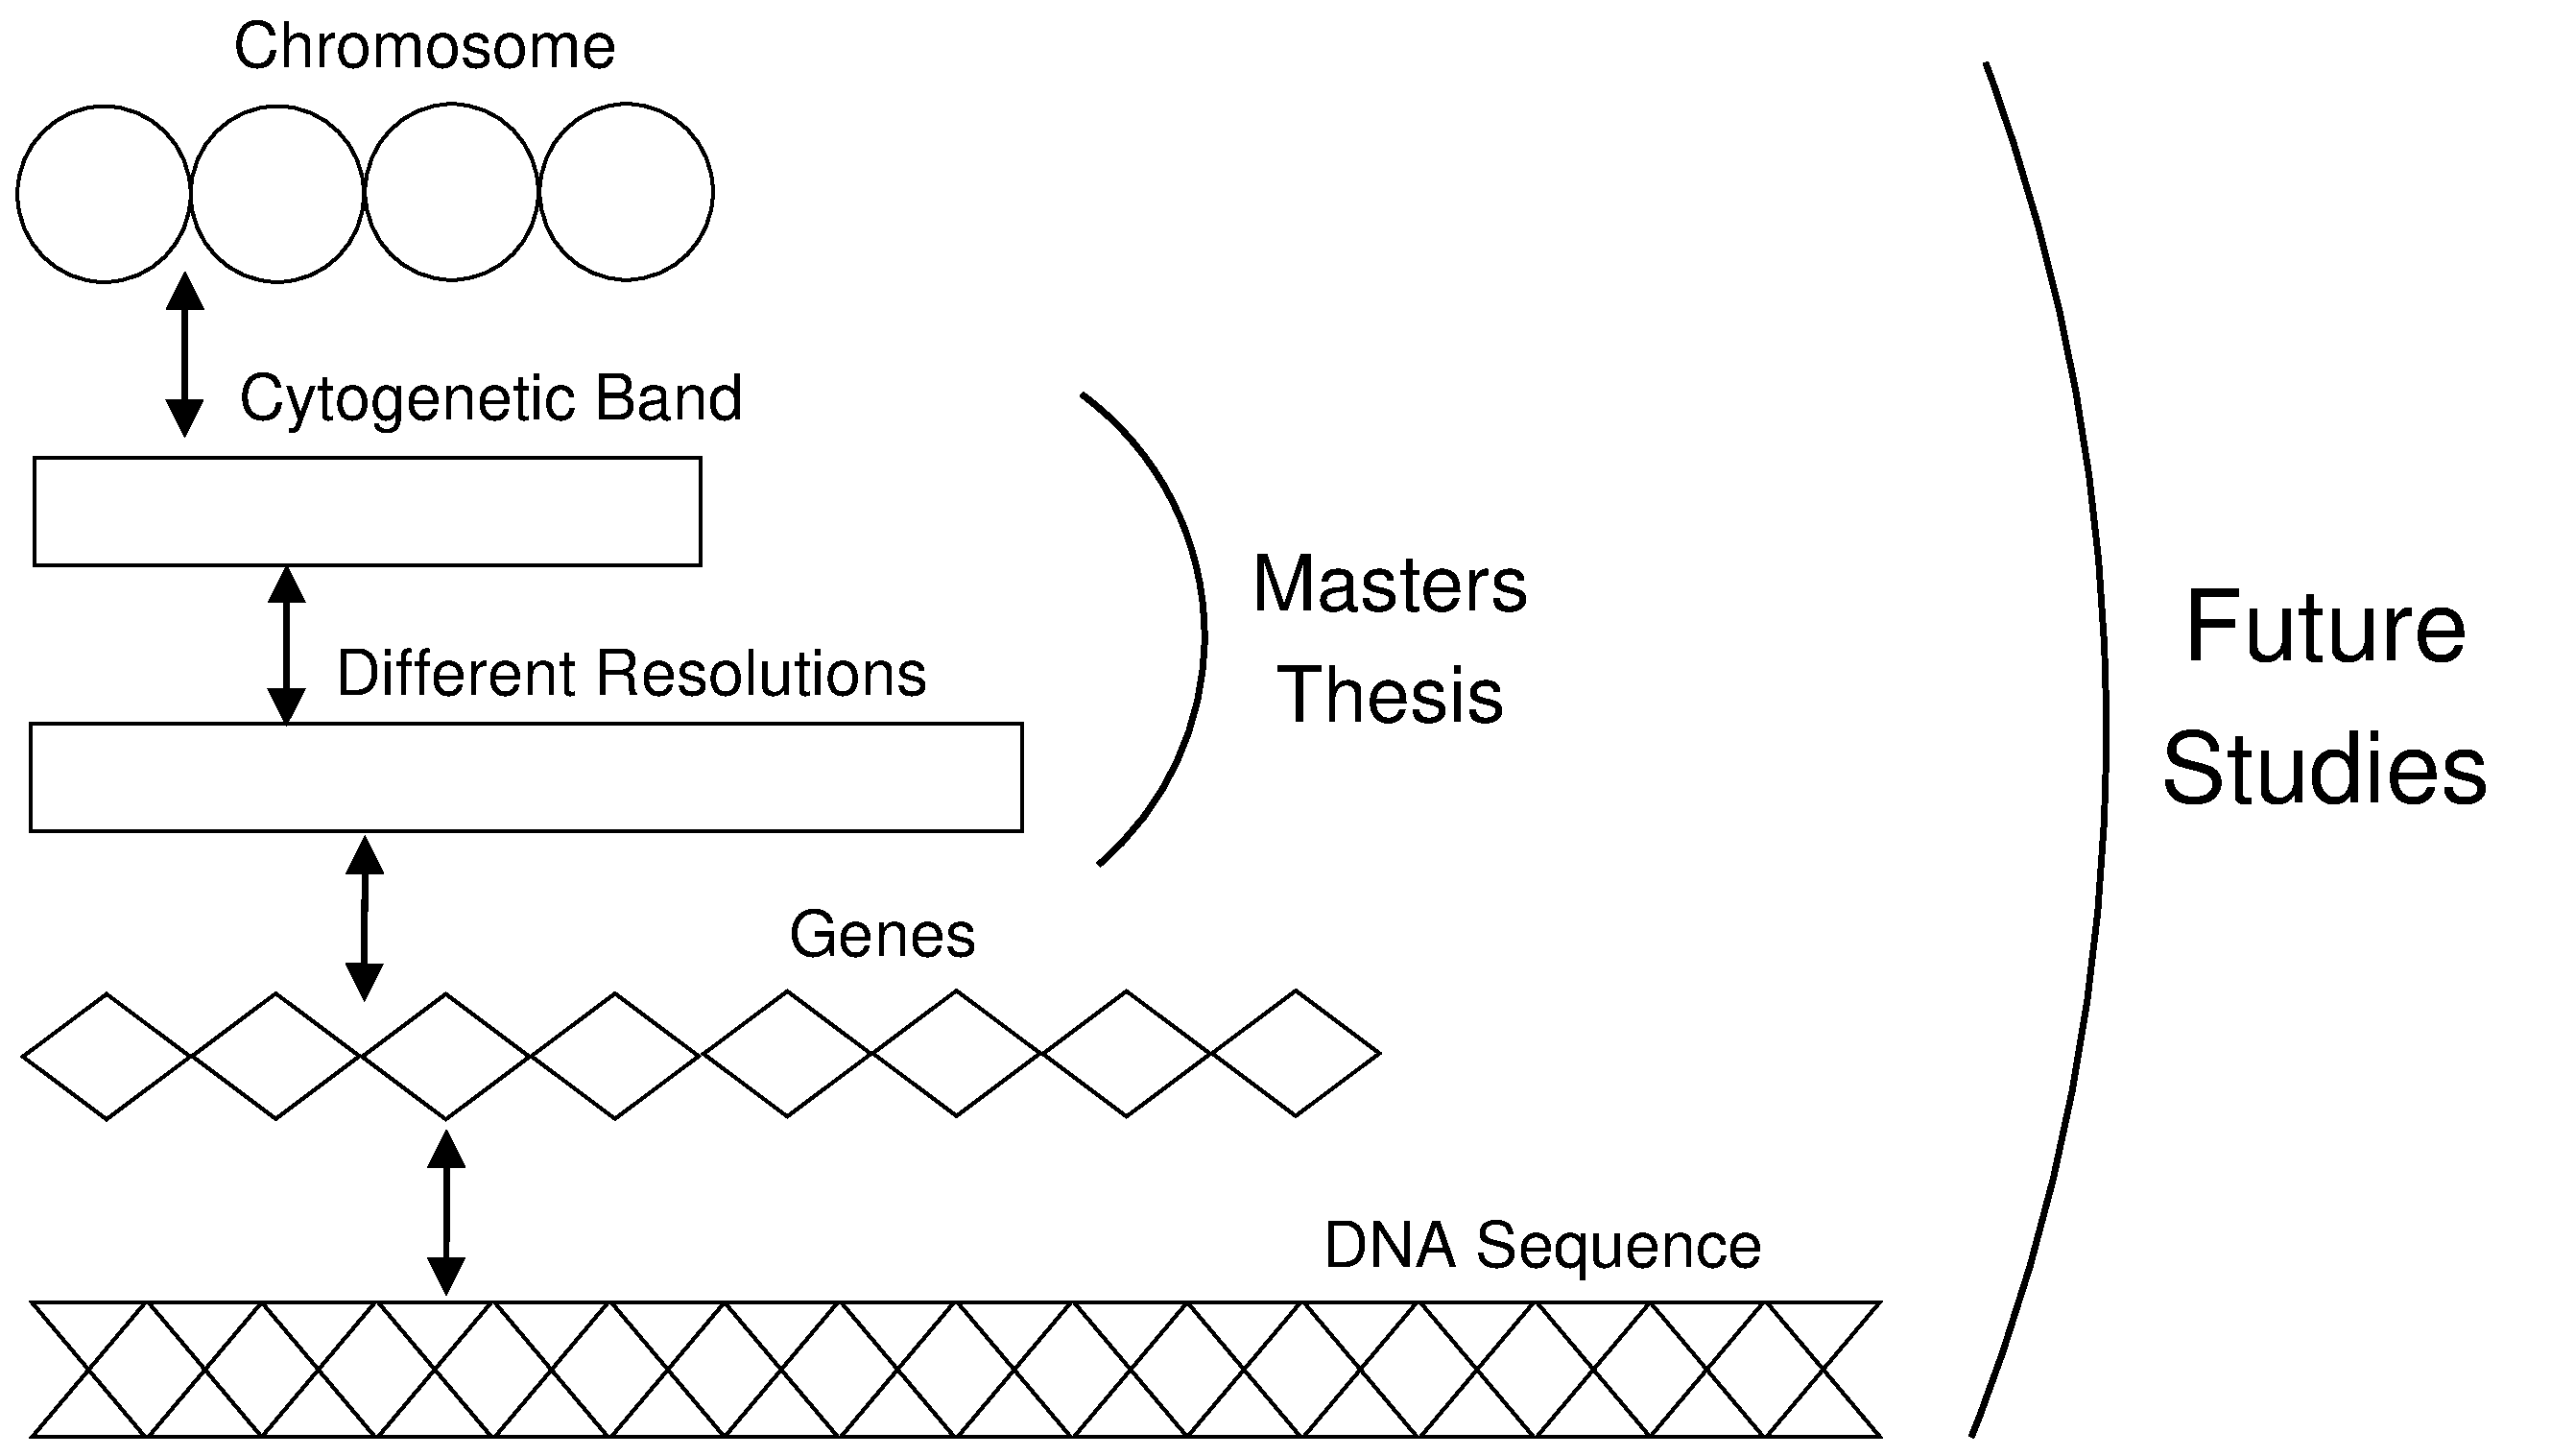
\includegraphics[width = 0.75\textwidth]{figures/problem}
\caption[Problem studied in the Master's thesis]{Schematic representation of problem studied in the Master's thesis and its seamless extension to the problem to be studied in future.} \label{Fig:problem}
\end{figure}

% As shown in Figure \ref{Fig:problem} this thesis focused on data transformation methods for changing the representation of the data in different resolution with the goal of database integration. The mixture modelling approach was then applied to the data in a single resolution. However, the field still lacks many methods and algorithms that can enhance the analysis of data in multiple resolutions without the need for transformation between different resolutions. The field seeks the  design and implementation of a multiresolution mixture model to work with multiple resolution of the data simultaneously. as shown in Figure \ref{Fig:solution}. 
% %\clearpage
% 
% \begin{figure}[h!]
% \centering
% \includegraphics[width = 0.9\textwidth]{figures/modeltry}
% \caption[Solution studied in Master's thesis]{Pictorial representation of the solution to the problem shown in Figure \ref{Fig:problem} achieved in Master's thesis and the possible solution for future studies.} \label{Fig:solution}
% \end{figure}

The multiresolution problem was studied only at chromosome level and the data transformation process was defined only in different resolutions of the chromosome. In the future work, the data transformation process can be defined until the very minute biological details such as genes and DNA sequences. Upsampling technique used in the thesis also needs further investigation and inferencing techniques can be implemented. In further work the probabilistic models, such as mixture models and probabilistic time series models, such as Hidden Markov Models(HMMs) can be extended to cope with data in multiple resolutions. 		%chap 6
\clearpage
\pagestyle{plain}
\input{src/bib.tex}		%chap 6

\clearpage 		%start new page flushing all previous data

% BIBLIOGRAPHY
%\bibliographystyle{styles/authordate1_ti} %modified :: www.ctan.org/tex-archive/biblio/bibtex/contrib/authordate/
%\bibliographystyle{unsrt}
% If you want ``REFERENCES'' to be ``Bibliography'', uncomment the following
%\renewcommand{\bibtitle}{Bibliography}
%\renewcommand{\bibheadtitle}{Bibliography}

%\bibliography{src/cv}
%\addcontentsline{toc}{chapter}{Bibliography}
%\clearpage

% APPENDICES
\appendix
\chapter{Chromosome Nomenclature}
\label{ap:appendNom}

\begin{fquote}[Ludwig Wittgenstein]If people never did silly things, nothing intelligent would ever get done. \fqsource{{Austrian philosopher (1889 - 1951)}} \end{fquote} 

There is a standardized naming scheme or nomenclature to address the different areas in the genome defined by the International System for Human Cytogenetic Nomenclature (ISCN) \cite{iscn}. This naming scheme is used by the domain experts and found in the literature when addressing the parts of the genome. The history of chromosome nomenclature dates back to 1971 when a meeting in Paris decided the basic nomenclature for the bands in the chromosome. Hence, the nomenclature is often referred to as Paris nomenclature and some names have been adopted from French.

A chromosome is divided into two arms by the centromere: the p arm which stands for petit (meaning small in French)  is the longer arm and the arm q which stands for queue. The regions are named q1, q2, q3 or p1, p2, p3 starting from the centromere and moving towards the edges. Regions are often separated by specific and consistent landmarks which possess distinct morphological characters such as the ends of the chromosome arms, the centromere and certain bands. The regions are further divided into bands such as q11 (pronounced as ‘q-one-one’ not ‘q-eleven’). The bands are further divided into sub-bands such as q11.1 or even sub-sub bands such as q11.11. This naming scheme is hierarchical and irregular.

\begin{figure}[h!]
\centering
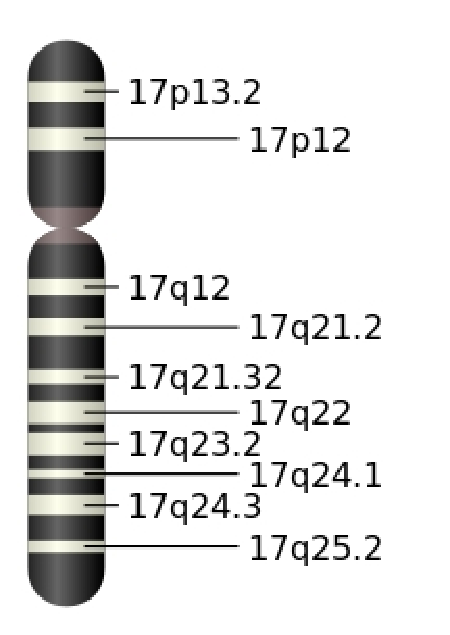
\includegraphics[width=0.4\textwidth]{figures/chromonomen}
\caption[Regions in chromosome 17 and resolution 400]{Nomenclature of Chromosome bands of Chromosome 17 in resolution 400.} \label{Fig:chromonomen}
\end{figure}

An example of chromosome nomenclature is shown in Figure \ref{Fig:chromonomen} which is an example case in chromosome 17. For example, area 17q21.32 means chromosome 17, arm ‘Q', region 21, band 3 and sub-band 2. It is important to note that length of each region, band and sub-band varies.

ISCN has also defined Ideograms for G-banding patterns for normal human chromosomes at five different resolutions \cite{iscn}. Five different resolutions of chromosomes mean that a chromosome is divided into different parts in different resolutions. In resolution 400, for example, the chromosome is divided into 393 different parts and in resolution 850, chromosome is divided in 862 different parts. With respect to the chromosome bands region q21 in resolution 400, for example, is divided into q21.1, q21.2, q21.31, q21.32 and q21.33 in resolution 850. However, region q22 in resolution 400 remains undivided in resolution 850 as well. The division of the chromosome bands is determined by the resolution of naming scheme which depends on the properties of the genome.
\chapter{Results on Each Chromosome}
\label{ap:appendRslt}

%\begin{tabular}{|c|c|r|c|r|c|r|}\hline
%    & $J$ & \multicolumn{1}{|c|}{\textbf{$\mathcal{L}$}} & $J$ & \multicolumn{1}{|c|}{\textbf{$\mathcal{L}$}} &$J$ & \multicolumn{1}{|c|}{\textbf{$\mathcal{L}$}}   \\ \hline%
 %\end{tabular}


\begin{fquote}[Tony Robbins]There is no such thing as failure. There are only results. \fqsource{{American self-help author(1960-)}} \end{fquote} 

\begin{synopsis}
This chapter presents a summary of results of experiments on all 22 chromosomes. Number of components required to fit the data ($J$) along with their respective likelihood ($\mathcal{L}$) in all three types of data: upsampled, downsampled and combined are also reported.
\end{synopsis}

\begin{table}[h!]
  \centering
\begin{tabular}{|c|c|r|c|r|c|r|}\hline
\multicolumn{7}{|c|}{\textbf{Chromosome 1}} \\ \hline
\multirow{2}{*}{\textbf{Resolution}} & \multicolumn{2}{|c|}{\textbf{Upsampled}} &  \multicolumn{2}{|c|}{\textbf{Downsampled}} &  \multicolumn{2}{|c|}{\textbf{Combined}} \\ \cline{2-7}
    & $J$ & \multicolumn{1}{|c|}{\textbf{$\mathcal{L}$}} & $J$ & \multicolumn{1}{|c|}{\textbf{$\mathcal{L}$}} & $J$ & \multicolumn{1}{|c|}{\textbf{$\mathcal{L}$}}   \\ \hline
400 & 6 & -5.9194 & 7 & -7.0697 & 7 & -7.0344  \\ \hline
550 & 7 & -12.9252 & 8 & -9.9172 & 8 & -9.9790  \\ \hline
700 & 7 & -16.4747 & 9 & -12.399 & 8 & -13.1283  \\ \hline
850 & 7 & -14.6505& 5 & -13.065 & 7 & -13.7521  \\ \hline
\end{tabular}
\end{table}

\clearpage

\begin{table}[h!]
  \centering
\begin{tabular}{|c|c|r|c|r|c|r|}\hline
\multicolumn{7}{|c|}{\textbf{Chromosome 2}} \\ \hline
\multirow{2}{*}{\textbf{Resolution}} & \multicolumn{2}{|c|}{\textbf{Upsampled}} &  \multicolumn{2}{|c|}{\textbf{Downsampled}} &  \multicolumn{2}{|c|}{\textbf{Combined}} \\ \cline{2-7}
    & $J$ & \multicolumn{1}{|c|}{\textbf{$\mathcal{L}$}} & $J$ & \multicolumn{1}{|c|}{\textbf{$\mathcal{L}$}} &$J$ & \multicolumn{1}{|c|}{\textbf{$\mathcal{L}$}}   \\ \hline
400 & 4 & -6.0295 & 7 & -8.0169 & 6 & -8.1897  \\ \hline
550 & 5 & -11.8613 & 7 & -11.7851 & 7 & -11.6974  \\ \hline
700 & 7 & -16.5517 & 7 & -13.4636 & 7 & -13.4568  \\ \hline
850 & 7 & -20.3705 & 7 & -15.0203 & 7 &  -16.5597 \\ \hline
\end{tabular}
\end{table}



\begin{table}[h!]
  \centering
\begin{tabular}{|c|c|r|c|r|c|r|}\hline
\multicolumn{7}{|c|}{\textbf{Chromosome 3}} \\ \hline
\multirow{2}{*}{\textbf{Resolution}} & \multicolumn{2}{|c|}{\textbf{Upsampled}} &  \multicolumn{2}{|c|}{\textbf{Downsampled}} &  \multicolumn{2}{|c|}{\textbf{Combined}} \\ \cline{2-7}
    & $J$ & \multicolumn{1}{|c|}{\textbf{$\mathcal{L}$}} & $J$ & \multicolumn{1}{|c|}{\textbf{$\mathcal{L}$}} &$J$ & \multicolumn{1}{|c|}{\textbf{$\mathcal{L}$}}   \\ \hline
400 & 4 & -6.2442 & 6 & -7.0561 & 7 & -6.7363  \\ \hline
550 & 7 & -7.6133 & 6 & -8.7447 & 7 & -8.4167  \\ \hline
700 & 4 & -10.4383 & 7 & -10.5652 & 6 & -11.2252  \\ \hline
850 & 7 & -12.4494 & 7 & -11.9871 & 7 & -12.9220  \\ \hline
\end{tabular}
\end{table}

\begin{table}[h!]
  \centering
\begin{tabular}{|c|c|r|c|r|c|r|}\hline
\multicolumn{7}{|c|}{\textbf{Chromosome 4}} \\ \hline
\multirow{2}{*}{\textbf{Resolution}} & \multicolumn{2}{|c|}{\textbf{Upsampled}} &  \multicolumn{2}{|c|}{\textbf{Downsampled}} &  \multicolumn{2}{|c|}{\textbf{Combined}} \\ \cline{2-7}
    & $J$ & \multicolumn{1}{|c|}{\textbf{$\mathcal{L}$}} & $J$ & \multicolumn{1}{|c|}{\textbf{$\mathcal{L}$}} &$J$ & \multicolumn{1}{|c|}{\textbf{$\mathcal{L}$}}   \\ \hline
400 & 6 & -5.5425 & 7 & -6.7628 & 8 & -6.5087  \\ \hline
550 & 4 & -7.3582 & 6 & -6.9300 & 8 & -7.1889  \\ \hline
700 & 3 & -14.3333 & 7 & -11.7569 & 7 & -12.3751  \\ \hline
850 & 6 & -14.3317 & 6 & -11.3934 & 7 & -11.6412   \\ \hline
\end{tabular}
\end{table}

\begin{table}[h!]
  \centering
\begin{tabular}{|c|c|r|c|r|c|r|}\hline
\multicolumn{7}{|c|}{\textbf{Chromosome 5}} \\ \hline
\multirow{2}{*}{\textbf{Resolution}} & \multicolumn{2}{|c|}{\textbf{Upsampled}} &  \multicolumn{2}{|c|}{\textbf{Downsampled}} &  \multicolumn{2}{|c|}{\textbf{Combined}} \\ \cline{2-7}
    & $J$ & \multicolumn{1}{|c|}{\textbf{$\mathcal{L}$}} & $J$ & \multicolumn{1}{|c|}{\textbf{$\mathcal{L}$}} &$J$ & \multicolumn{1}{|c|}{\textbf{$\mathcal{L}$}}   \\ \hline
400 & 5 & -3.8016 & 7 & -5.2970 & 7 & -5.2339  \\ \hline
550 & 4 & -12.158 & 8 & -9.3618 & 6 & -9.5914  \\ \hline
700 & 8 & -21.0161 & 7 & -12.6904 & 7 & -12.4653  \\ \hline
850 & 6 & -20.7898 & 6 & -12.8497 & 7 & -13.0176  \\ \hline
\end{tabular}
\end{table}

\begin{table}[h!]
  \centering
\begin{tabular}{|c|c|r|c|r|c|r|}\hline
\multicolumn{7}{|c|}{\textbf{Chromosome 6}} \\ \hline
\multirow{2}{*}{\textbf{Resolution}} & \multicolumn{2}{|c|}{\textbf{Upsampled}} &  \multicolumn{2}{|c|}{\textbf{Downsampled}} &  \multicolumn{2}{|c|}{\textbf{Combined}} \\ \cline{2-7}
    & $J$ & \multicolumn{1}{|c|}{\textbf{$\mathcal{L}$}} & $J$ & \multicolumn{1}{|c|}{\textbf{$\mathcal{L}$}} &$J$ & \multicolumn{1}{|c|}{\textbf{$\mathcal{L}$}}   \\ \hline
400 & 3 & -6.8321 & 7 & -6.0988 & 6 & -6.4244  \\ \hline
550 & 5 & -9.3474 & 7 & -8.2348 & 6 & -8.8388  \\ \hline
700 & 4 & -14.9753 & 6 & -10.317 & 6 & -11.9083  \\ \hline
850 & 6 & -17.0915 & 6 & -12.560 & 5 & -13.1997  \\ \hline
\end{tabular}
\end{table}



\begin{table}[h!]
  \centering
\begin{tabular}{|c|c|r|c|r|c|r|}\hline
\multicolumn{7}{|c|}{\textbf{Chromosome 7}} \\ \hline
\multirow{2}{*}{\textbf{Resolution}} & \multicolumn{2}{|c|}{\textbf{Upsampled}} &  \multicolumn{2}{|c|}{\textbf{Downsampled}} &  \multicolumn{2}{|c|}{\textbf{Combined}} \\ \cline{2-7}
    & $J$ & \multicolumn{1}{|c|}{\textbf{$\mathcal{L}$}} & $J$ & \multicolumn{1}{|c|}{\textbf{$\mathcal{L}$}} &$J$ & \multicolumn{1}{|c|}{\textbf{$\mathcal{L}$}}   \\ \hline
400 & 7 & -4.7596 & 7 & -4.4072 & 6 & -4.8041  \\ \hline
550 & 7 & -6.4318 & 7 & -5.6954 & 7 & -5.9767  \\ \hline
700 & 5 & -12.160 & 7 & -7.5511 & 5 & -8.8348  \\ \hline
850 & 4 & -18.9840 & 4 & -8.6133 & 7 & -9.7109  \\ \hline
\end{tabular}
\end{table}

\begin{table}[h!]
  \centering
\begin{tabular}{|c|c|r|c|r|c|r|}\hline
\multicolumn{7}{|c|}{\textbf{Chromosome 8}} \\ \hline
\multirow{2}{*}{\textbf{Resolution}} & \multicolumn{2}{|c|}{\textbf{Upsampled}} &  \multicolumn{2}{|c|}{\textbf{Downsampled}} &  \multicolumn{2}{|c|}{\textbf{Combined}} \\ \cline{2-7}
    & $J$ & \multicolumn{1}{|c|}{\textbf{$\mathcal{L}$}} & $J$ & \multicolumn{1}{|c|}{\textbf{$\mathcal{L}$}} &$J$ & \multicolumn{1}{|c|}{\textbf{$\mathcal{L}$}}   \\ \hline
400 & 4 & -4.9276 & 6 & -4.1155 & 6 & -4.3724  \\ \hline
550 & 4 & -6.2317 & 7 & -4.9172 & 6 & -5.3038  \\ \hline
700 & 4 & -10.5181 & 7 & -7.1678 & 7 & -7.4469  \\ \hline
850 & 8 & -8.1046 & 8 & -7.1619 & 7 & -7.4235  \\ \hline
\end{tabular}
\end{table}

\begin{table}[h!]
  \centering
\begin{tabular}{|c|c|r|c|r|c|r|}\hline
\multicolumn{7}{|c|}{\textbf{Chromosome 9}} \\ \hline
\multirow{2}{*}{\textbf{Resolution}} & \multicolumn{2}{|c|}{\textbf{Upsampled}} &  \multicolumn{2}{|c|}{\textbf{Downsampled}} &  \multicolumn{2}{|c|}{\textbf{Combined}} \\ \cline{2-7}
    & $J$ & \multicolumn{1}{|c|}{\textbf{$\mathcal{L}$}} & $J$ & \multicolumn{1}{|c|}{\textbf{$\mathcal{L}$}} &$J$ & \multicolumn{1}{|c|}{\textbf{$\mathcal{L}$}}   \\ \hline
400 & 6 & -3.8209 & 7 & -4.3096 & 5 & -4.7419  \\ \hline
550 & 5 & -5.2903 & 7 & -4.9811 & 6 & -5.5177  \\ \hline
700 & 8 & -10.620 & 6 & -8.6071 & 5 & -9.5910  \\ \hline
850 & 7 & -10.0603 & 7 & -9.5175 & 6 & -9.5272  \\ \hline
\end{tabular}
\end{table}

\clearpage

\begin{table}[h!]
  \centering
\begin{tabular}{|c|c|r|c|r|c|r|}\hline
\multicolumn{7}{|c|}{\textbf{Chromosome 10}} \\ \hline
\multirow{2}{*}{\textbf{Resolution}} & \multicolumn{2}{|c|}{\textbf{Upsampled}} &  \multicolumn{2}{|c|}{\textbf{Downsampled}} &  \multicolumn{2}{|c|}{\textbf{Combined}} \\ \cline{2-7}
    & $J$ & \multicolumn{1}{|c|}{\textbf{$\mathcal{L}$}} & $J$ & \multicolumn{1}{|c|}{\textbf{$\mathcal{L}$}} &$J$ & \multicolumn{1}{|c|}{\textbf{$\mathcal{L}$}}   \\ \hline
400 & 8 & -3.2834 & 6 & -4.3964 & 6 & -4.3978  \\ \hline
550 & 8 & -2.7821 & 7 & -6.3721 & 7 & -6.2640  \\ \hline
700 & 8 & -8.8074 & 8 & -8.2315 & 6 & -9.0516  \\ \hline
850 & 8 & -13.3051 & 8 & -11.1141 & 6 & -11.0203  \\ \hline
\end{tabular}
\end{table}



\begin{table}[h!]
  \centering
\begin{tabular}{|c|c|r|c|r|c|r|}\hline
\multicolumn{7}{|c|}{\textbf{Chromosome 11}} \\ \hline
\multirow{2}{*}{\textbf{Resolution}} & \multicolumn{2}{|c|}{\textbf{Upsampled}} &  \multicolumn{2}{|c|}{\textbf{Downsampled}} &  \multicolumn{2}{|c|}{\textbf{Combined}} \\ \cline{2-7}
    & $J$ & \multicolumn{1}{|c|}{\textbf{$\mathcal{L}$}} & $J$ & \multicolumn{1}{|c|}{\textbf{$\mathcal{L}$}} &$J$ & \multicolumn{1}{|c|}{\textbf{$\mathcal{L}$}}   \\ \hline
400 & 4 & -3.6813 & 6 & -4.7850 & 6 & -4.7648  \\ \hline
550 & 8 & -3.9603 & 8 & -7.5050 & 6 & -8.1162  \\ \hline
700 & 4 & -15.6520 & 7 & -11.1570 & 6 & -11.4460  \\ \hline
850 & 4 & -13.3610 & 4 & -11.2810 & 9 & -11.4400  \\ \hline
\end{tabular}
\end{table}

\begin{table}[h!]
  \centering
\begin{tabular}{|c|c|r|c|r|c|r|}\hline
\multicolumn{7}{|c|}{\textbf{Chromosome 12}} \\ \hline
\multirow{2}{*}{\textbf{Resolution}} & \multicolumn{2}{|c|}{\textbf{Upsampled}} &  \multicolumn{2}{|c|}{\textbf{Downsampled}} &  \multicolumn{2}{|c|}{\textbf{Combined}} \\ \cline{2-7}
    & $J$ & \multicolumn{1}{|c|}{\textbf{$\mathcal{L}$}} & $J$ & \multicolumn{1}{|c|}{\textbf{$\mathcal{L}$}} &$J$ & \multicolumn{1}{|c|}{\textbf{$\mathcal{L}$}}   \\ \hline
400 & 6 & -4.1444 & 7 & -4.6736 & 8 & -4.6166  \\ \hline
550 & 8 & -5.0504 & 8 & -6.2282 & 8 & -6.3146  \\ \hline
700 & 6 & -13.9440 & 7 & -10.961 & 9 & -10.5580 \\ \hline
850 & 5 & -16.9440 & 5 & -10.738 & 10 & -10.7330  \\ \hline
\end{tabular}
\end{table}

\begin{table}[h!]
  \centering
\begin{tabular}{|c|c|r|c|r|c|r|}\hline
\multicolumn{7}{|c|}{\textbf{Chromosome 13}} \\ \hline
\multirow{2}{*}{\textbf{Resolution}} & \multicolumn{2}{|c|}{\textbf{Upsampled}} &  \multicolumn{2}{|c|}{\textbf{Downsampled}} &  \multicolumn{2}{|c|}{\textbf{Combined}} \\ \cline{2-7}
    & $J$ & \multicolumn{1}{|c|}{\textbf{$\mathcal{L}$}} & $J$ & \multicolumn{1}{|c|}{\textbf{$\mathcal{L}$}} &$J$ & \multicolumn{1}{|c|}{\textbf{$\mathcal{L}$}}   \\ \hline
400 & 5 & -3.6969 & 6 & -3.4472 & 7 & -3.3926  \\ \hline
550 & 5 & -4.3378 & 8 & -3.8797 & 9 & -3.7812  \\ \hline
700 & 9 & -3.9688 & 7 & -4.7221 & 8 & -4.6245  \\ \hline
850 & 6 & -8.7558 & 6 & -7.3815 & 6 & -7.9231  \\ \hline
\end{tabular}
\end{table}

\clearpage

\begin{table}[h!]
  \centering
\begin{tabular}{|c|c|r|c|r|c|r|}\hline
\multicolumn{7}{|c|}{\textbf{Chromosome 14}} \\ \hline
\multirow{2}{*}{\textbf{Resolution}} & \multicolumn{2}{|c|}{\textbf{Upsampled}} &  \multicolumn{2}{|c|}{\textbf{Downsampled}} &  \multicolumn{2}{|c|}{\textbf{Combined}} \\ \cline{2-7}
    & $J$ & \multicolumn{1}{|c|}{\textbf{$\mathcal{L}$}} & $J$ & \multicolumn{1}{|c|}{\textbf{$\mathcal{L}$}} &$J$ & \multicolumn{1}{|c|}{\textbf{$\mathcal{L}$}}   \\ \hline
400 & 5 & -3.7348 & 6 & -3.4965 & 6 & -3.4845  \\ \hline
550 & 5 & -4.3009 & 6 & -3.7693 & 8 & -3.6269  \\ \hline
700 & 7 & -4.6961 & 7 & -4.3075 & 7 & -4.3181  \\ \hline
850 & 4 & -7.6186 & 4 & -6.0092 & 7 & -5.6381  \\ \hline
\end{tabular}
\end{table}



\begin{table}[h!]
  \centering
\begin{tabular}{|c|c|r|c|r|c|r|}\hline
\multicolumn{7}{|c|}{\textbf{Chromosome 15}} \\ \hline
\multirow{2}{*}{\textbf{Resolution}} & \multicolumn{2}{|c|}{\textbf{Upsampled}} &  \multicolumn{2}{|c|}{\textbf{Downsampled}} &  \multicolumn{2}{|c|}{\textbf{Combined}} \\ \cline{2-7}
    & $J$ & \multicolumn{1}{|c|}{\textbf{$\mathcal{L}$}} & $J$ & \multicolumn{1}{|c|}{\textbf{$\mathcal{L}$}} &$J$ & \multicolumn{1}{|c|}{\textbf{$\mathcal{L}$}}   \\ \hline
400 & 6 & -3.1646 & 5 & -3.8836 & 8 & -3.4694  \\ \hline
550 & 4 & -4.9117 & 9 & -4.1355 & 7 & -4.4979  \\ \hline
700 & 5 & -4.8904 & 9 & -4.4926 & 7 & -4.8368 \\ \hline
850 & 8 & -4.3434 & 8 & -6.3936 & 8 & -5.5853  \\ \hline
\end{tabular}
\end{table}

\begin{table}[h!]
  \centering
\begin{tabular}{|c|c|r|c|r|c|r|}\hline
\multicolumn{7}{|c|}{\textbf{Chromosome 16}} \\ \hline
\multirow{2}{*}{\textbf{Resolution}} & \multicolumn{2}{|c|}{\textbf{Upsampled}} &  \multicolumn{2}{|c|}{\textbf{Downsampled}} &  \multicolumn{2}{|c|}{\textbf{Combined}} \\ \cline{2-7}
    & $J$ & \multicolumn{1}{|c|}{\textbf{$\mathcal{L}$}} & $J$ & \multicolumn{1}{|c|}{\textbf{$\mathcal{L}$}} &$J$ & \multicolumn{1}{|c|}{\textbf{$\mathcal{L}$}}   \\ \hline
400 & 5 & -3.5699 & 4 & -3.7158   & 6 & -3.3564  \\ \hline
550 & 7 & -3.1739 & 6 & -3.3044   & 6 & -3.3510  \\ \hline
700 & 5 & -4.7573 & 6 & -4.0875   & 6 & -4.1563  \\ \hline
850 & 11 & -3.3864 & 11 & -4.5890 & 6 & -4.6062  \\ \hline
\end{tabular}
\end{table}

\begin{table}[h!]
  \centering
\begin{tabular}{|c|c|r|c|r|c|r|}\hline
\multicolumn{7}{|c|}{\textbf{Chromosome 17}} \\ \hline
\multirow{2}{*}{\textbf{Resolution}} & \multicolumn{2}{|c|}{\textbf{Upsampled}} &  \multicolumn{2}{|c|}{\textbf{Downsampled}} &  \multicolumn{2}{|c|}{\textbf{Combined}} \\ \cline{2-7}
    & $J$ & \multicolumn{1}{|c|}{\textbf{$\mathcal{L}$}} & $J$ & \multicolumn{1}{|c|}{\textbf{$\mathcal{L}$}} &$J$ & \multicolumn{1}{|c|}{\textbf{$\mathcal{L}$}}   \\ \hline
400 & 6 & -3.3910 & 7 & -3.2701 & 6 & -3.4884  \\ \hline
550 & 8 & -3.2570 & 7 & -3.4897 & 7 & -3.5734  \\ \hline
700 & 6 & -4.4526 & 6 & -4.7788 & 8 & -4.4173  \\ \hline
850 & 8 & -4.3136 & 8 & -4.5374 & 6 & -5.2015  \\ \hline
\end{tabular}
\end{table}

\clearpage

\begin{table}[h!]
  \centering
\begin{tabular}{|c|c|r|c|r|c|r|}\hline
\multicolumn{7}{|c|}{\textbf{Chromosome 18}} \\ \hline
\multirow{2}{*}{\textbf{Resolution}} & \multicolumn{2}{|c|}{\textbf{Upsampled}} &  \multicolumn{2}{|c|}{\textbf{Downsampled}} &  \multicolumn{2}{|c|}{\textbf{Combined}} \\ \cline{2-7}
    & $J$ & \multicolumn{1}{|c|}{\textbf{$\mathcal{L}$}} & $J$ & \multicolumn{1}{|c|}{\textbf{$\mathcal{L}$}} &$J$ & \multicolumn{1}{|c|}{\textbf{$\mathcal{L}$}}   \\ \hline
400 & 4 & -3.4651 & 7 & -2.5073 & 6 & -2.7273  \\ \hline
550 & 5 & -3.5862 & 7 & -3.0942 & 6 & -3.2695  \\ \hline
700 & 6 & -3.5142 & 6 & -3.2159 & 7 & -3.2043  \\ \hline
850 & 9 & -3.6741 & 9 & -3.8413 & 7 & -3.7792  \\ \hline
\end{tabular}
\end{table}



\begin{table}[h!]
  \centering
\begin{tabular}{|c|c|r|c|r|c|r|}\hline
\multicolumn{7}{|c|}{\textbf{Chromosome 19}} \\ \hline
\multirow{2}{*}{\textbf{Resolution}} & \multicolumn{2}{|c|}{\textbf{Upsampled}} &  \multicolumn{2}{|c|}{\textbf{Downsampled}} &  \multicolumn{2}{|c|}{\textbf{Combined}} \\ \cline{2-7}
    & $J$ & \multicolumn{1}{|c|}{\textbf{$\mathcal{L}$}} & $J$ & \multicolumn{1}{|c|}{\textbf{$\mathcal{L}$}} &$J$ & \multicolumn{1}{|c|}{\textbf{$\mathcal{L}$}}   \\ \hline
400 & 3 & -3.7135 & 6 & -2.4045 & 6 & -2.5358  \\ \hline
550 & 5 & -2.8951 & 6 & -2.4154 & 7 & -2.4565  \\ \hline
700 & 4 & -5.1835 & 6 & -2.9831 & 7 & -3.0044  \\ \hline
850 & 4 & -4.0183 & 4 & -3.0227 & 5 & -3.3670  \\ \hline
\end{tabular}
\end{table}

\begin{table}[h!]
  \centering
\begin{tabular}{|c|c|r|c|r|c|r|}\hline
\multicolumn{7}{|c|}{\textbf{Chromosome 20}} \\ \hline
\multirow{2}{*}{\textbf{Resolution}} & \multicolumn{2}{|c|}{\textbf{Upsampled}} &  \multicolumn{2}{|c|}{\textbf{Downsampled}} &  \multicolumn{2}{|c|}{\textbf{Combined}} \\ \cline{2-7}
    & $J$ & \multicolumn{1}{|c|}{\textbf{$\mathcal{L}$}} & $J$ & \multicolumn{1}{|c|}{\textbf{$\mathcal{L}$}} &$J$ & \multicolumn{1}{|c|}{\textbf{$\mathcal{L}$}}   \\ \hline
400 & 5 & -2.9799 & 6 & -2.4055 & 6 & -2.5126  \\ \hline
550 & 6 & -2.9034 & 6 & -2.2939 & 6 & -2.5126  \\ \hline
700 & 5 & -3.6122 & 7 & -2.6078 & 6 & -2.9454  \\ \hline
850 & 5 & -4.0085 & 5 & -3.1918 & 7 & -3.1907 \\ \hline
\end{tabular}
\end{table}

\begin{table}[h!]
  \centering
\begin{tabular}{|c|c|r|c|r|c|r|}\hline
\multicolumn{7}{|c|}{\textbf{Chromosome 21}} \\ \hline
\multirow{2}{*}{\textbf{Resolution}} & \multicolumn{2}{|c|}{\textbf{Upsampled}} &  \multicolumn{2}{|c|}{\textbf{Downsampled}} &  \multicolumn{2}{|c|}{\textbf{Combined}} \\ \cline{2-7}
    & $J$ & \multicolumn{1}{|c|}{\textbf{$\mathcal{L}$}} & $J$ & \multicolumn{1}{|c|}{\textbf{$\mathcal{L}$}} &$J$ & \multicolumn{1}{|c|}{\textbf{$\mathcal{L}$}}   \\ \hline
400 & 4 & -1.6774 & 5 & -1.5461 & 5 & -1.6076  \\ \hline
550 & 6 & -1.6447 & 4 & -1.8109 & 5 & -1.7402  \\ \hline
700 & 5 & -2.1391 & 5 & -1.9207 & 7 & -1.7489  \\ \hline
850 & 5 & -2.1391 & 5 & -1.8478 & 6 & -2.0233  \\ \hline
\end{tabular}
\end{table}

\clearpage

\begin{table}[h!]
  \centering
\begin{tabular}{|c|c|r|c|r|c|r|}\hline
\multicolumn{7}{|c|}{\textbf{Chromosome 22}} \\ \hline
\multirow{2}{*}{\textbf{Resolution}} & \multicolumn{2}{|c|}{\textbf{Upsampled}} &  \multicolumn{2}{|c|}{\textbf{Downsampled}} &  \multicolumn{2}{|c|}{\textbf{Combined}} \\ \cline{2-7}
    & $J$ & \multicolumn{1}{|c|}{\textbf{$\mathcal{L}$}} & $J$ & \multicolumn{1}{|c|}{\textbf{$\mathcal{L}$}} &$J$ & \multicolumn{1}{|c|}{\textbf{$\mathcal{L}$}}   \\ \hline
400 & 7 & -2.1946 & 4 & -1.7142 & 3 & -1.9641  \\ \hline
550 & 7 & -2.2315 & 5 & -2.1204 & 4 & -2.3481  \\ \hline
700 & 7 & -2.7416 & 6 & -2.4106 & 5 & -2.5080  \\ \hline
850 & 8 & -2.4068 & 8 & -2.4156 & 7 & -2.3680  \\ \hline
\end{tabular}
\end{table}


%\begin{table}[h!]
%  \centering
%\begin{tabular}{|@{}c@{}|@{}l@{}|@{}c@{}|@{}c@{}|} \hline
%\centering

%\multicolumn{4}{|c|}{\textbf{Chromosome 1}} \\ \hline
%\textbf{Resolution} & \textbf{Data Type} &  \textbf{\# of Components} & \textbf{Likelihood} \\ \hline %\cline{2-7}
  
%\multirow{3}{*}{\textbf{300}} & Downsampled & 7 & -0.1143  \\ \cline{2-4}
% & Upsampled & 7 & -0.1143  \\ \cline{2-4}
% & Combined & 7 & -0.1143  \\ \hline

%\multirow{3}{*}{\textbf{400}} & Downsampled & 7 & -0.1143  \\ \cline{2-4}
% & Upsampled & 7 & -0.1143  \\ \cline{2-4}
% & Combined & 7 & -0.1143  \\ \hline


%\end{tabular}
%\end{table}





\input{src/appendData.tex}

%\backmatter %ending pages
%\label{page:lastpage}

% end of document
\end{document}
